\documentclass[twoside]{book}

% Packages required by doxygen
\usepackage{fixltx2e}
\usepackage{calc}
\usepackage{doxygen}
\usepackage[export]{adjustbox} % also loads graphicx
\usepackage{graphicx}
\usepackage[utf8]{inputenc}
\usepackage{makeidx}
\usepackage{multicol}
\usepackage{multirow}
\PassOptionsToPackage{warn}{textcomp}
\usepackage{textcomp}
\usepackage[nointegrals]{wasysym}
\usepackage[table]{xcolor}

% Font selection
\usepackage[T1]{fontenc}
\usepackage[scaled=.90]{helvet}
\usepackage{courier}
\usepackage{amssymb}
\usepackage{sectsty}
\renewcommand{\familydefault}{\sfdefault}
\allsectionsfont{%
  \fontseries{bc}\selectfont%
  \color{darkgray}%
}
\renewcommand{\DoxyLabelFont}{%
  \fontseries{bc}\selectfont%
  \color{darkgray}%
}
\newcommand{\+}{\discretionary{\mbox{\scriptsize$\hookleftarrow$}}{}{}}

% Page & text layout
\usepackage{geometry}
\geometry{%
  a4paper,%
  top=2.5cm,%
  bottom=2.5cm,%
  left=2.5cm,%
  right=2.5cm%
}
\tolerance=750
\hfuzz=15pt
\hbadness=750
\setlength{\emergencystretch}{15pt}
\setlength{\parindent}{0cm}
\setlength{\parskip}{3ex plus 2ex minus 2ex}
\makeatletter
\renewcommand{\paragraph}{%
  \@startsection{paragraph}{4}{0ex}{-1.0ex}{1.0ex}{%
    \normalfont\normalsize\bfseries\SS@parafont%
  }%
}
\renewcommand{\subparagraph}{%
  \@startsection{subparagraph}{5}{0ex}{-1.0ex}{1.0ex}{%
    \normalfont\normalsize\bfseries\SS@subparafont%
  }%
}
\makeatother

% Headers & footers
\usepackage{fancyhdr}
\pagestyle{fancyplain}
\fancyhead[LE]{\fancyplain{}{\bfseries\thepage}}
\fancyhead[CE]{\fancyplain{}{}}
\fancyhead[RE]{\fancyplain{}{\bfseries\leftmark}}
\fancyhead[LO]{\fancyplain{}{\bfseries\rightmark}}
\fancyhead[CO]{\fancyplain{}{}}
\fancyhead[RO]{\fancyplain{}{\bfseries\thepage}}
\fancyfoot[LE]{\fancyplain{}{}}
\fancyfoot[CE]{\fancyplain{}{}}
\fancyfoot[RE]{\fancyplain{}{\bfseries\scriptsize Generated by Doxygen }}
\fancyfoot[LO]{\fancyplain{}{\bfseries\scriptsize Generated by Doxygen }}
\fancyfoot[CO]{\fancyplain{}{}}
\fancyfoot[RO]{\fancyplain{}{}}
\renewcommand{\footrulewidth}{0.4pt}
\renewcommand{\chaptermark}[1]{%
  \markboth{#1}{}%
}
\renewcommand{\sectionmark}[1]{%
  \markright{\thesection\ #1}%
}

% Indices & bibliography
\usepackage{natbib}
\usepackage[titles]{tocloft}
\setcounter{tocdepth}{3}
\setcounter{secnumdepth}{5}
\makeindex

% Hyperlinks (required, but should be loaded last)
\usepackage{ifpdf}
\ifpdf
  \usepackage[pdftex,pagebackref=true]{hyperref}
\else
  \usepackage[ps2pdf,pagebackref=true]{hyperref}
\fi
\hypersetup{%
  colorlinks=true,%
  linkcolor=blue,%
  citecolor=blue,%
  unicode%
}

% Custom commands
\newcommand{\clearemptydoublepage}{%
  \newpage{\pagestyle{empty}\cleardoublepage}%
}

\usepackage{caption}
\captionsetup{labelsep=space,justification=centering,font={bf},singlelinecheck=off,skip=4pt,position=top}

%===== C O N T E N T S =====

\begin{document}

% Titlepage & ToC
\hypersetup{pageanchor=false,
             bookmarksnumbered=true,
             pdfencoding=unicode
            }
\pagenumbering{roman}
\begin{titlepage}
\vspace*{7cm}
\begin{center}%
{\Large Markov Model of Keyboard Tokens \\[1ex]\large 0 }\\
\vspace*{1cm}
{\large Generated by Doxygen 1.8.11}\\
\end{center}
\end{titlepage}
\clearemptydoublepage
\tableofcontents
\clearemptydoublepage
\pagenumbering{arabic}
\hypersetup{pageanchor=true}

%--- Begin generated contents ---
\chapter{Namespace Index}
\section{Packages}
Here are the packages with brief descriptions (if available)\+:\begin{DoxyCompactList}
\item\contentsline{section}{\hyperlink{namespacecomponents}{components} }{\pageref{namespacecomponents}}{}
\item\contentsline{section}{\hyperlink{namespacedata__analysis}{data\+\_\+analysis} }{\pageref{namespacedata__analysis}}{}
\item\contentsline{section}{\hyperlink{namespacegui}{gui} }{\pageref{namespacegui}}{}
\item\contentsline{section}{\hyperlink{namespacejunit}{junit} }{\pageref{namespacejunit}}{}
\item\contentsline{section}{\hyperlink{namespacerank}{rank} }{\pageref{namespacerank}}{}
\item\contentsline{section}{\hyperlink{namespaceruntime}{runtime} }{\pageref{namespaceruntime}}{}
\item\contentsline{section}{\hyperlink{namespacetest}{test} }{\pageref{namespacetest}}{}
\item\contentsline{section}{\hyperlink{namespacetrie}{trie} }{\pageref{namespacetrie}}{}
\end{DoxyCompactList}

\chapter{Hierarchical Index}
\section{Class Hierarchy}
This inheritance list is sorted roughly, but not completely, alphabetically\+:\begin{DoxyCompactList}
\item \contentsline{section}{components.\+Chain}{\pageref{classcomponents_1_1_chain}}{}
\item \contentsline{section}{runtime.\+Chain\+Builder}{\pageref{classruntime_1_1_chain_builder}}{}
\item Comparable\begin{DoxyCompactList}
\item \contentsline{section}{components.\+Touch}{\pageref{classcomponents_1_1_touch}}{}
\item \contentsline{section}{components.\+Window}{\pageref{classcomponents_1_1_window}}{}
\end{DoxyCompactList}
\item \contentsline{section}{runtime.\+Chain\+Builder.\+Compare\+Method}{\pageref{enumruntime_1_1_chain_builder_1_1_compare_method}}{}
\item \contentsline{section}{rank.\+Complete\+Probability}{\pageref{classrank_1_1_complete_probability}}{}
\item \contentsline{section}{runtime.\+Operation\+\_\+thread.\+Computation}{\pageref{enumruntime_1_1_operation__thread_1_1_computation}}{}
\item \contentsline{section}{test.\+Main.\+Test\+Files.\+Concentration}{\pageref{enumtest_1_1_main_1_1_test_files_1_1_concentration}}{}
\item \contentsline{section}{test.\+Main.\+Test\+Files.\+Distribution}{\pageref{enumtest_1_1_main_1_1_test_files_1_1_distribution}}{}
\item \contentsline{section}{components.\+Distribution}{\pageref{classcomponents_1_1_distribution}}{}
\item \contentsline{section}{test.\+Main}{\pageref{classtest_1_1_main}}{}
\item \contentsline{section}{data\+\_\+analysis.\+Model\+\_\+compare}{\pageref{classdata__analysis_1_1_model__compare}}{}
\item \contentsline{section}{test.\+Main.\+Test\+Files.\+Pressure\+Amount}{\pageref{enumtest_1_1_main_1_1_test_files_1_1_pressure_amount}}{}
\item \contentsline{section}{test.\+Print\+\_\+model}{\pageref{classtest_1_1_print__model}}{}
\item Runnable\begin{DoxyCompactList}
\item \contentsline{section}{data\+\_\+analysis.\+Model\+\_\+compare\+\_\+thread}{\pageref{classdata__analysis_1_1_model__compare__thread}}{}
\item \contentsline{section}{runtime.\+Compare\+Chains}{\pageref{classruntime_1_1_compare_chains}}{}
\begin{DoxyCompactList}
\item \contentsline{section}{rank.\+Compare\+Chains\+Rank}{\pageref{classrank_1_1_compare_chains_rank}}{}
\end{DoxyCompactList}
\item \contentsline{section}{runtime.\+Operation\+\_\+thread}{\pageref{classruntime_1_1_operation__thread}}{}
\end{DoxyCompactList}
\item \contentsline{section}{gui.\+Start\+G\+UI}{\pageref{classgui_1_1_start_g_u_i}}{}
\item \contentsline{section}{runtime.\+Chain\+Builder.\+State}{\pageref{enumruntime_1_1_chain_builder_1_1_state}}{}
\item \contentsline{section}{data\+\_\+analysis.\+Statistics}{\pageref{classdata__analysis_1_1_statistics}}{}
\item \contentsline{section}{components.\+Token}{\pageref{classcomponents_1_1_token}}{}
\item \contentsline{section}{trie.\+Trie}{\pageref{classtrie_1_1_trie}}{}
\item \contentsline{section}{components.\+Token.\+Type}{\pageref{enumcomponents_1_1_token_1_1_type}}{}
\item \contentsline{section}{junit.\+Unit\+\_\+\+Compare\+Chains\+Rank}{\pageref{classjunit_1_1_unit___compare_chains_rank}}{}
\item \contentsline{section}{junit.\+Unit\+\_\+\+Complete\+Probability}{\pageref{classjunit_1_1_unit___complete_probability}}{}
\item \contentsline{section}{test.\+Unit\+Compare\+Chains\+Rank}{\pageref{classtest_1_1_unit_compare_chains_rank}}{}
\item \contentsline{section}{test.\+Unit\+Rank\+Compare}{\pageref{classtest_1_1_unit_rank_compare}}{}
\item Array\+List\begin{DoxyCompactList}
\item \contentsline{section}{trie.\+Trie\+List}{\pageref{classtrie_1_1_trie_list}}{}
\end{DoxyCompactList}
\item J\+Frame\begin{DoxyCompactList}
\item \contentsline{section}{gui.\+Marcov\+\_\+frame}{\pageref{classgui_1_1_marcov__frame}}{}
\end{DoxyCompactList}
\item J\+Panel\begin{DoxyCompactList}
\item \contentsline{section}{gui.\+Marcov\+\_\+console\+\_\+panel}{\pageref{classgui_1_1_marcov__console__panel}}{}
\item \contentsline{section}{gui.\+Marcov\+\_\+file\+\_\+display\+\_\+panel}{\pageref{classgui_1_1_marcov__file__display__panel}}{}
\item \contentsline{section}{gui.\+Marcov\+\_\+options\+\_\+panel}{\pageref{classgui_1_1_marcov__options__panel}}{}
\end{DoxyCompactList}
\end{DoxyCompactList}

\chapter{Class Index}
\section{Class List}
Here are the classes, structs, unions and interfaces with brief descriptions\+:\begin{DoxyCompactList}
\item\contentsline{section}{\hyperlink{classcomponents_1_1_chain}{components.\+Chain} }{\pageref{classcomponents_1_1_chain}}{}
\item\contentsline{section}{\hyperlink{classruntime_1_1_chain_builder}{runtime.\+Chain\+Builder} }{\pageref{classruntime_1_1_chain_builder}}{}
\item\contentsline{section}{\hyperlink{classruntime_1_1_compare_chains}{runtime.\+Compare\+Chains} \\*This thread will call the compare method of chain class. The goal is to compare user chain and auth chain and make the result, pass/fail known. Or do something based on pass/fail such as cause the phone to lock }{\pageref{classruntime_1_1_compare_chains}}{}
\item\contentsline{section}{\hyperlink{classrank_1_1_compare_chains_rank}{rank.\+Compare\+Chains\+Rank} }{\pageref{classrank_1_1_compare_chains_rank}}{}
\item\contentsline{section}{\hyperlink{enumruntime_1_1_chain_builder_1_1_compare_method}{runtime.\+Chain\+Builder.\+Compare\+Method} }{\pageref{enumruntime_1_1_chain_builder_1_1_compare_method}}{}
\item\contentsline{section}{\hyperlink{classrank_1_1_complete_probability}{rank.\+Complete\+Probability} }{\pageref{classrank_1_1_complete_probability}}{}
\item\contentsline{section}{\hyperlink{enumruntime_1_1_operation__thread_1_1_computation}{runtime.\+Operation\+\_\+thread.\+Computation} }{\pageref{enumruntime_1_1_operation__thread_1_1_computation}}{}
\item\contentsline{section}{\hyperlink{enumtest_1_1_main_1_1_test_files_1_1_concentration}{test.\+Main.\+Test\+Files.\+Concentration} }{\pageref{enumtest_1_1_main_1_1_test_files_1_1_concentration}}{}
\item\contentsline{section}{\hyperlink{enumtest_1_1_main_1_1_test_files_1_1_distribution}{test.\+Main.\+Test\+Files.\+Distribution} }{\pageref{enumtest_1_1_main_1_1_test_files_1_1_distribution}}{}
\item\contentsline{section}{\hyperlink{classcomponents_1_1_distribution}{components.\+Distribution} }{\pageref{classcomponents_1_1_distribution}}{}
\item\contentsline{section}{\hyperlink{classtest_1_1_main}{test.\+Main} }{\pageref{classtest_1_1_main}}{}
\item\contentsline{section}{\hyperlink{classgui_1_1_marcov__console__panel}{gui.\+Marcov\+\_\+console\+\_\+panel} }{\pageref{classgui_1_1_marcov__console__panel}}{}
\item\contentsline{section}{\hyperlink{classgui_1_1_marcov__file__display__panel}{gui.\+Marcov\+\_\+file\+\_\+display\+\_\+panel} }{\pageref{classgui_1_1_marcov__file__display__panel}}{}
\item\contentsline{section}{\hyperlink{classgui_1_1_marcov__frame}{gui.\+Marcov\+\_\+frame} }{\pageref{classgui_1_1_marcov__frame}}{}
\item\contentsline{section}{\hyperlink{classgui_1_1_marcov__options__panel}{gui.\+Marcov\+\_\+options\+\_\+panel} }{\pageref{classgui_1_1_marcov__options__panel}}{}
\item\contentsline{section}{\hyperlink{classdata__analysis_1_1_model__compare}{data\+\_\+analysis.\+Model\+\_\+compare} }{\pageref{classdata__analysis_1_1_model__compare}}{}
\item\contentsline{section}{\hyperlink{classdata__analysis_1_1_model__compare__thread}{data\+\_\+analysis.\+Model\+\_\+compare\+\_\+thread} }{\pageref{classdata__analysis_1_1_model__compare__thread}}{}
\item\contentsline{section}{\hyperlink{classruntime_1_1_operation__thread}{runtime.\+Operation\+\_\+thread} }{\pageref{classruntime_1_1_operation__thread}}{}
\item\contentsline{section}{\hyperlink{enumtest_1_1_main_1_1_test_files_1_1_pressure_amount}{test.\+Main.\+Test\+Files.\+Pressure\+Amount} }{\pageref{enumtest_1_1_main_1_1_test_files_1_1_pressure_amount}}{}
\item\contentsline{section}{\hyperlink{classtest_1_1_print__model}{test.\+Print\+\_\+model} }{\pageref{classtest_1_1_print__model}}{}
\item\contentsline{section}{\hyperlink{classgui_1_1_start_g_u_i}{gui.\+Start\+G\+UI} }{\pageref{classgui_1_1_start_g_u_i}}{}
\item\contentsline{section}{\hyperlink{enumruntime_1_1_chain_builder_1_1_state}{runtime.\+Chain\+Builder.\+State} }{\pageref{enumruntime_1_1_chain_builder_1_1_state}}{}
\item\contentsline{section}{\hyperlink{classdata__analysis_1_1_statistics}{data\+\_\+analysis.\+Statistics} }{\pageref{classdata__analysis_1_1_statistics}}{}
\item\contentsline{section}{\hyperlink{classcomponents_1_1_token}{components.\+Token} }{\pageref{classcomponents_1_1_token}}{}
\item\contentsline{section}{\hyperlink{classcomponents_1_1_touch}{components.\+Touch} \\*This class represents a touch event }{\pageref{classcomponents_1_1_touch}}{}
\item\contentsline{section}{\hyperlink{classtrie_1_1_trie}{trie.\+Trie} }{\pageref{classtrie_1_1_trie}}{}
\item\contentsline{section}{\hyperlink{classtrie_1_1_trie_list}{trie.\+Trie\+List} }{\pageref{classtrie_1_1_trie_list}}{}
\item\contentsline{section}{\hyperlink{enumcomponents_1_1_token_1_1_type}{components.\+Token.\+Type} \\*Specify the type of token we want to build }{\pageref{enumcomponents_1_1_token_1_1_type}}{}
\item\contentsline{section}{\hyperlink{classjunit_1_1_unit___compare_chains_rank}{junit.\+Unit\+\_\+\+Compare\+Chains\+Rank} }{\pageref{classjunit_1_1_unit___compare_chains_rank}}{}
\item\contentsline{section}{\hyperlink{classjunit_1_1_unit___complete_probability}{junit.\+Unit\+\_\+\+Complete\+Probability} }{\pageref{classjunit_1_1_unit___complete_probability}}{}
\item\contentsline{section}{\hyperlink{classtest_1_1_unit_compare_chains_rank}{test.\+Unit\+Compare\+Chains\+Rank} }{\pageref{classtest_1_1_unit_compare_chains_rank}}{}
\item\contentsline{section}{\hyperlink{classtest_1_1_unit_rank_compare}{test.\+Unit\+Rank\+Compare} }{\pageref{classtest_1_1_unit_rank_compare}}{}
\item\contentsline{section}{\hyperlink{classcomponents_1_1_window}{components.\+Window} \\*This class will store and provide functions for a single window within the model }{\pageref{classcomponents_1_1_window}}{}
\end{DoxyCompactList}

\chapter{File Index}
\section{File List}
Here is a list of all files with brief descriptions\+:\begin{DoxyCompactList}
\item\contentsline{section}{/home/element/\+P\+U\+F/\+Keyboard/java\+\_\+scripts/java\+\_\+marcov\+\_\+model/src/components/\hyperlink{_chain_8java}{Chain.\+java} }{\pageref{_chain_8java}}{}
\item\contentsline{section}{/home/element/\+P\+U\+F/\+Keyboard/java\+\_\+scripts/java\+\_\+marcov\+\_\+model/src/components/\hyperlink{_distribution_8java}{Distribution.\+java} }{\pageref{_distribution_8java}}{}
\item\contentsline{section}{/home/element/\+P\+U\+F/\+Keyboard/java\+\_\+scripts/java\+\_\+marcov\+\_\+model/src/components/\hyperlink{_token_8java}{Token.\+java} }{\pageref{_token_8java}}{}
\item\contentsline{section}{/home/element/\+P\+U\+F/\+Keyboard/java\+\_\+scripts/java\+\_\+marcov\+\_\+model/src/components/\hyperlink{_touch_8java}{Touch.\+java} }{\pageref{_touch_8java}}{}
\item\contentsline{section}{/home/element/\+P\+U\+F/\+Keyboard/java\+\_\+scripts/java\+\_\+marcov\+\_\+model/src/components/\hyperlink{_window_8java}{Window.\+java} }{\pageref{_window_8java}}{}
\item\contentsline{section}{/home/element/\+P\+U\+F/\+Keyboard/java\+\_\+scripts/java\+\_\+marcov\+\_\+model/src/data\+\_\+analysis/\hyperlink{_model__compare_8java}{Model\+\_\+compare.\+java} }{\pageref{_model__compare_8java}}{}
\item\contentsline{section}{/home/element/\+P\+U\+F/\+Keyboard/java\+\_\+scripts/java\+\_\+marcov\+\_\+model/src/data\+\_\+analysis/\hyperlink{_model__compare__thread_8java}{Model\+\_\+compare\+\_\+thread.\+java} }{\pageref{_model__compare__thread_8java}}{}
\item\contentsline{section}{/home/element/\+P\+U\+F/\+Keyboard/java\+\_\+scripts/java\+\_\+marcov\+\_\+model/src/data\+\_\+analysis/\hyperlink{_statistics_8java}{Statistics.\+java} }{\pageref{_statistics_8java}}{}
\item\contentsline{section}{/home/element/\+P\+U\+F/\+Keyboard/java\+\_\+scripts/java\+\_\+marcov\+\_\+model/src/gui/\hyperlink{_marcov__console__panel_8java}{Marcov\+\_\+console\+\_\+panel.\+java} }{\pageref{_marcov__console__panel_8java}}{}
\item\contentsline{section}{/home/element/\+P\+U\+F/\+Keyboard/java\+\_\+scripts/java\+\_\+marcov\+\_\+model/src/gui/\hyperlink{_marcov__file__display__panel_8java}{Marcov\+\_\+file\+\_\+display\+\_\+panel.\+java} }{\pageref{_marcov__file__display__panel_8java}}{}
\item\contentsline{section}{/home/element/\+P\+U\+F/\+Keyboard/java\+\_\+scripts/java\+\_\+marcov\+\_\+model/src/gui/\hyperlink{_marcov__frame_8java}{Marcov\+\_\+frame.\+java} }{\pageref{_marcov__frame_8java}}{}
\item\contentsline{section}{/home/element/\+P\+U\+F/\+Keyboard/java\+\_\+scripts/java\+\_\+marcov\+\_\+model/src/gui/\hyperlink{_marcov__options__panel_8java}{Marcov\+\_\+options\+\_\+panel.\+java} }{\pageref{_marcov__options__panel_8java}}{}
\item\contentsline{section}{/home/element/\+P\+U\+F/\+Keyboard/java\+\_\+scripts/java\+\_\+marcov\+\_\+model/src/gui/\hyperlink{_start_g_u_i_8java}{Start\+G\+U\+I.\+java} }{\pageref{_start_g_u_i_8java}}{}
\item\contentsline{section}{/home/element/\+P\+U\+F/\+Keyboard/java\+\_\+scripts/java\+\_\+marcov\+\_\+model/src/junit/\hyperlink{_unit___compare_chains_rank_8java}{Unit\+\_\+\+Compare\+Chains\+Rank.\+java} }{\pageref{_unit___compare_chains_rank_8java}}{}
\item\contentsline{section}{/home/element/\+P\+U\+F/\+Keyboard/java\+\_\+scripts/java\+\_\+marcov\+\_\+model/src/junit/\hyperlink{_unit___complete_probability_8java}{Unit\+\_\+\+Complete\+Probability.\+java} }{\pageref{_unit___complete_probability_8java}}{}
\item\contentsline{section}{/home/element/\+P\+U\+F/\+Keyboard/java\+\_\+scripts/java\+\_\+marcov\+\_\+model/src/rank/\hyperlink{_compare_chains_rank_8java}{Compare\+Chains\+Rank.\+java} }{\pageref{_compare_chains_rank_8java}}{}
\item\contentsline{section}{/home/element/\+P\+U\+F/\+Keyboard/java\+\_\+scripts/java\+\_\+marcov\+\_\+model/src/rank/\hyperlink{_complete_probability_8java}{Complete\+Probability.\+java} }{\pageref{_complete_probability_8java}}{}
\item\contentsline{section}{/home/element/\+P\+U\+F/\+Keyboard/java\+\_\+scripts/java\+\_\+marcov\+\_\+model/src/runtime/\hyperlink{_chain_builder_8java}{Chain\+Builder.\+java} }{\pageref{_chain_builder_8java}}{}
\item\contentsline{section}{/home/element/\+P\+U\+F/\+Keyboard/java\+\_\+scripts/java\+\_\+marcov\+\_\+model/src/runtime/\hyperlink{_compare_chains_8java}{Compare\+Chains.\+java} }{\pageref{_compare_chains_8java}}{}
\item\contentsline{section}{/home/element/\+P\+U\+F/\+Keyboard/java\+\_\+scripts/java\+\_\+marcov\+\_\+model/src/runtime/\hyperlink{_operation__thread_8java}{Operation\+\_\+thread.\+java} }{\pageref{_operation__thread_8java}}{}
\item\contentsline{section}{/home/element/\+P\+U\+F/\+Keyboard/java\+\_\+scripts/java\+\_\+marcov\+\_\+model/src/test/\hyperlink{_main_8java}{Main.\+java} }{\pageref{_main_8java}}{}
\item\contentsline{section}{/home/element/\+P\+U\+F/\+Keyboard/java\+\_\+scripts/java\+\_\+marcov\+\_\+model/src/test/\hyperlink{_print__model_8java}{Print\+\_\+model.\+java} }{\pageref{_print__model_8java}}{}
\item\contentsline{section}{/home/element/\+P\+U\+F/\+Keyboard/java\+\_\+scripts/java\+\_\+marcov\+\_\+model/src/test/\hyperlink{_unit_compare_chains_rank_8java}{Unit\+Compare\+Chains\+Rank.\+java} }{\pageref{_unit_compare_chains_rank_8java}}{}
\item\contentsline{section}{/home/element/\+P\+U\+F/\+Keyboard/java\+\_\+scripts/java\+\_\+marcov\+\_\+model/src/test/\hyperlink{_unit_rank_compare_8java}{Unit\+Rank\+Compare.\+java} }{\pageref{_unit_rank_compare_8java}}{}
\item\contentsline{section}{/home/element/\+P\+U\+F/\+Keyboard/java\+\_\+scripts/java\+\_\+marcov\+\_\+model/src/test/\hyperlink{_utilities_8java}{Utilities.\+java} }{\pageref{_utilities_8java}}{}
\item\contentsline{section}{/home/element/\+P\+U\+F/\+Keyboard/java\+\_\+scripts/java\+\_\+marcov\+\_\+model/src/trie/\hyperlink{_trie_8java}{Trie.\+java} }{\pageref{_trie_8java}}{}
\item\contentsline{section}{/home/element/\+P\+U\+F/\+Keyboard/java\+\_\+scripts/java\+\_\+marcov\+\_\+model/src/trie/\hyperlink{_trie_list_8java}{Trie\+List.\+java} }{\pageref{_trie_list_8java}}{}
\end{DoxyCompactList}

\chapter{Namespace Documentation}
\hypertarget{namespacecomponents}{}\section{Package components}
\label{namespacecomponents}\index{components@{components}}
\subsection*{Classes}
\begin{DoxyCompactItemize}
\item 
class \hyperlink{classcomponents_1_1_chain}{Chain}
\item 
class \hyperlink{classcomponents_1_1_distribution}{Distribution}
\item 
class \hyperlink{classcomponents_1_1_token}{Token}
\item 
class \hyperlink{classcomponents_1_1_touch}{Touch}
\begin{DoxyCompactList}\small\item\em This class represents a touch event. \end{DoxyCompactList}\item 
class \hyperlink{classcomponents_1_1_window}{Window}
\begin{DoxyCompactList}\small\item\em This class will store and provide functions for a single window within the model. \end{DoxyCompactList}\end{DoxyCompactItemize}

\hypertarget{namespacedata__analysis}{}\section{Package data\+\_\+analysis}
\label{namespacedata__analysis}\index{data\+\_\+analysis@{data\+\_\+analysis}}
\subsection*{Classes}
\begin{DoxyCompactItemize}
\item 
class \hyperlink{classdata__analysis_1_1_model__compare}{Model\+\_\+compare}
\begin{DoxyCompactList}\small\item\em Analysis class used to compare and analyze data gathered from users. \end{DoxyCompactList}\item 
class \hyperlink{classdata__analysis_1_1_model__compare__thread}{Model\+\_\+compare\+\_\+thread}
\begin{DoxyCompactList}\small\item\em Compare Markov Chains on their own thread. \end{DoxyCompactList}\item 
class \hyperlink{classdata__analysis_1_1_statistics}{Statistics}
\begin{DoxyCompactList}\small\item\em Generates statistics on results generated by model\+\_\+compare.\+java. \end{DoxyCompactList}\end{DoxyCompactItemize}

\hypertarget{namespacegui}{}\section{Package gui}
\label{namespacegui}\index{gui@{gui}}
\subsection*{Classes}
\begin{DoxyCompactItemize}
\item 
class \hyperlink{classgui_1_1_marcov__console__panel}{Marcov\+\_\+console\+\_\+panel}
\item 
class \hyperlink{classgui_1_1_marcov__file__display__panel}{Marcov\+\_\+file\+\_\+display\+\_\+panel}
\item 
class \hyperlink{classgui_1_1_marcov__frame}{Marcov\+\_\+frame}
\item 
class \hyperlink{classgui_1_1_marcov__options__panel}{Marcov\+\_\+options\+\_\+panel}
\item 
class \hyperlink{classgui_1_1_start_g_u_i}{Start\+G\+UI}
\end{DoxyCompactItemize}

\hypertarget{namespacejunit}{}\section{Package junit}
\label{namespacejunit}\index{junit@{junit}}
\subsection*{Classes}
\begin{DoxyCompactItemize}
\item 
class \hyperlink{classjunit_1_1_unit___compare_chains_rank}{Unit\+\_\+\+Compare\+Chains\+Rank}
\begin{DoxyCompactList}\small\item\em goal is to test compare chains rank functionality \end{DoxyCompactList}\item 
class \hyperlink{classjunit_1_1_unit___complete_probability}{Unit\+\_\+\+Complete\+Probability}
\begin{DoxyCompactList}\small\item\em unit test demonstrating how to compute probility \end{DoxyCompactList}\end{DoxyCompactItemize}

\hypertarget{namespacerank}{}\section{Package rank}
\label{namespacerank}\index{rank@{rank}}
\subsection*{Classes}
\begin{DoxyCompactItemize}
\item 
class \hyperlink{classrank_1_1_compare_chains_rank}{Compare\+Chains\+Rank}
\item 
class \hyperlink{classrank_1_1_complete_probability}{Complete\+Probability}
\end{DoxyCompactItemize}

\hypertarget{namespaceruntime}{}\section{Package runtime}
\label{namespaceruntime}\index{runtime@{runtime}}
\subsection*{Classes}
\begin{DoxyCompactItemize}
\item 
class \hyperlink{classruntime_1_1_chain_builder}{Chain\+Builder}
\item 
class \hyperlink{classruntime_1_1_compare_chains}{Compare\+Chains}
\begin{DoxyCompactList}\small\item\em This thread will call the compare method of chain class. The goal is to compare user chain and auth chain and make the result, pass/fail known. Or do something based on pass/fail such as cause the phone to lock. \end{DoxyCompactList}\item 
class \hyperlink{classruntime_1_1_operation__thread}{Operation\+\_\+thread}
\end{DoxyCompactItemize}

\hypertarget{namespacetest}{}\section{Package test}
\label{namespacetest}\index{test@{test}}
\subsection*{Classes}
\begin{DoxyCompactItemize}
\item 
class \hyperlink{classtest_1_1_main}{Main}
\item 
class \hyperlink{classtest_1_1_print__model}{Print\+\_\+model}
\item 
class \hyperlink{classtest_1_1_unit_compare_chains_rank}{Unit\+Compare\+Chains\+Rank}
\item 
class \hyperlink{classtest_1_1_unit_rank_compare}{Unit\+Rank\+Compare}
\end{DoxyCompactItemize}

\hypertarget{namespacetrie}{}\section{Package trie}
\label{namespacetrie}\index{trie@{trie}}
\subsection*{Classes}
\begin{DoxyCompactItemize}
\item 
class \hyperlink{classtrie_1_1_trie}{Trie}
\begin{DoxyCompactList}\small\item\em Implementation of Prefix Tree. \end{DoxyCompactList}\item 
class \hyperlink{classtrie_1_1_trie_list}{Trie\+List}
\begin{DoxyCompactList}\small\item\em Wrapper around \hyperlink{classtrie_1_1_trie}{Trie} used to maintain an ordering among the stored elements. \end{DoxyCompactList}\end{DoxyCompactItemize}

\chapter{Class Documentation}
\hypertarget{classcomponents_1_1_chain}{}\section{components.\+Chain Class Reference}
\label{classcomponents_1_1_chain}\index{components.\+Chain@{components.\+Chain}}
\subsection*{Public Member Functions}
\begin{DoxyCompactItemize}
\item 
\hyperlink{classcomponents_1_1_chain_afd25b8fbf65a81889a812eeb63b9520e}{Chain} (int window, int token, int threshold, int model\+\_\+size)
\item 
\hyperlink{classcomponents_1_1_chain_ac35b83e35e0bd5295eb873e2a5a2f989}{Chain} (\hyperlink{classcomponents_1_1_chain}{Chain} c)
\begin{DoxyCompactList}\small\item\em copy constructor. New chain object should have the same state as the old with differant object references. \end{DoxyCompactList}\item 
void \hyperlink{classcomponents_1_1_chain_a9a8aa7996f3f4b65a0f0dbbddd84f14b}{add\+\_\+touch} (\hyperlink{classcomponents_1_1_touch}{Touch} touch)
\item 
void \hyperlink{classcomponents_1_1_chain_a2eb35304ee80f15c741a986a214e663b}{add\+\_\+touch\+\_\+list} (List$<$ \hyperlink{classcomponents_1_1_touch}{Touch} $>$ t)
\item 
void \hyperlink{classcomponents_1_1_chain_a4184b4a5a7bd8b2412e7543c2db91af1}{set\+\_\+distribution} (\hyperlink{classcomponents_1_1_distribution}{Distribution} distribution, List$<$ \hyperlink{classcomponents_1_1_distribution}{Distribution} $>$ key\+\_\+distribution)
\item 
double \hyperlink{classcomponents_1_1_chain_a96cec1762b6f69856f54aad9e37b04a7}{get\+\_\+touch\+\_\+probability} (\hyperlink{classcomponents_1_1_window}{Window} w, \hyperlink{classcomponents_1_1_touch}{Touch} t)
\begin{DoxyCompactList}\small\item\em returns the probability of a given touch (at the i\textquotesingle{}th index) based on the model. This will depend on the preceeding touches, in \hyperlink{classcomponents_1_1_window}{Window}. A request for one probability will necessarily result in all of the probabilities being computed. \end{DoxyCompactList}\item 
\hyperlink{classcomponents_1_1_distribution}{Distribution} \hyperlink{classcomponents_1_1_chain_ae3cf3859627624dd155cf1507514cf20}{get\+\_\+distribution} ()
\begin{DoxyCompactList}\small\item\em returns the distribution of the data as a whole \end{DoxyCompactList}\item 
List$<$ \hyperlink{classcomponents_1_1_distribution}{Distribution} $>$ \hyperlink{classcomponents_1_1_chain_a654c25d3edab107ad77710428f11280c}{get\+\_\+key\+\_\+distribution} ()
\begin{DoxyCompactList}\small\item\em returns a list of distributions for each key \end{DoxyCompactList}\item 
int \hyperlink{classcomponents_1_1_chain_a1eb6b4a7d6cb462910932e29b3ab732e}{get\+\_\+window} ()
\item 
int \hyperlink{classcomponents_1_1_chain_ac6aca5adf04bb1500c1d8735cd7d5881}{get\+\_\+token} ()
\item 
int \hyperlink{classcomponents_1_1_chain_a545c320b4e5cc5e150ec6b07f8870fa1}{get\+\_\+model\+\_\+size} ()
\item 
int \hyperlink{classcomponents_1_1_chain_a128ee372728530d787a9512350dad405}{get\+\_\+threshold} ()
\item 
void \hyperlink{classcomponents_1_1_chain_a620eea641b4a673af78000c2ef5af576}{reset} ()
\begin{DoxyCompactList}\small\item\em resets the object.. this is the same as constructing a new chain, but faster \end{DoxyCompactList}\item 
void \hyperlink{classcomponents_1_1_chain_a401a39b68da4ae8ba64e02af94e68f15}{compute\+\_\+uncomputed} ()
\begin{DoxyCompactList}\small\item\em computes all uncomputed aspects of the chain \end{DoxyCompactList}\item 
double \hyperlink{classcomponents_1_1_chain_ab23f30bde8f169d73c3a3e5588bf75c6}{compare\+\_\+to} (\hyperlink{classcomponents_1_1_chain}{Chain} auth\+\_\+chain)
\item 
boolean \hyperlink{classcomponents_1_1_chain_a8bb0e379e0102b0443c38ef174fe83cc}{is\+\_\+touch\+\_\+in\+\_\+key\+\_\+distribution} (\hyperlink{classcomponents_1_1_touch}{Touch} touch)
\begin{DoxyCompactList}\small\item\em returns true if a touch is within 2 sigma for it\textquotesingle{}s key distribution \end{DoxyCompactList}\item 
List$<$ \hyperlink{classcomponents_1_1_window}{Window} $>$ \hyperlink{classcomponents_1_1_chain_a48f2e0718eb4a400c6ceb23afb0ea162}{get\+\_\+windows} ()
\begin{DoxyCompactList}\small\item\em handle requests for windows \end{DoxyCompactList}\item 
List$<$ \hyperlink{classcomponents_1_1_token}{Token} $>$ \hyperlink{classcomponents_1_1_chain_aed8e3b1ca179438db491b35a2eee822b}{get\+\_\+tokens} ()
\begin{DoxyCompactList}\small\item\em handle requests for tokens \end{DoxyCompactList}\item 
List$<$ \hyperlink{classcomponents_1_1_touch}{Touch} $>$ \hyperlink{classcomponents_1_1_chain_affd01133384c5cb222448c76ab0a82fb}{get\+\_\+touches} ()
\begin{DoxyCompactList}\small\item\em get a list of all touches in the chain \end{DoxyCompactList}\item 
String \hyperlink{classcomponents_1_1_chain_ac5496e565687d95b78cbc2d34bbb2ba2}{to\+String} ()
\begin{DoxyCompactList}\small\item\em prints out all of the touches in order \end{DoxyCompactList}\item 
void \hyperlink{classcomponents_1_1_chain_acf107be5a3d4e0dc151f07e0c519f698}{output\+\_\+to\+\_\+csv} (String file\+\_\+name)
\begin{DoxyCompactList}\small\item\em N\+OT U\+S\+E\+F\+UL IN A\+N\+D\+R\+O\+ID. This is used for debugging purposes. Outputs the model to a csv file in a readable format. \end{DoxyCompactList}\end{DoxyCompactItemize}


\subsection{Detailed Description}
T\+O\+DO make the chain\textquotesingle{}s compare\+\_\+to method be able to update incrementally T\+O\+DO make sure to use get\+\_\+\+X\+X\+X\+X\+X\+X() instead of the instance variables T\+O\+DO put windows into a Trie data structure for building model faster T\+O\+DO anywhere where I need to compare windows, or Touches I need the option to do this with tokens there needs to be a way to set the distribution used for a chain. This is because the authentication chain is evaluated with the distribution of the base chain. compute the windows somewhere. This will be based on the threshold, window, token sizes. This may change distributions? if a touch is thrown out? this class represents the marcov chain. It contains a sequence of touches and a distribution. I avoid doing any processing on touch being added because eventually this will be called on key press in android. Setting it up this way is more flexible to in the sense that processing may be done at any time. caches the result of each computation so it does not have to be repeated. 

\subsection{Constructor \& Destructor Documentation}
\index{components\+::\+Chain@{components\+::\+Chain}!Chain@{Chain}}
\index{Chain@{Chain}!components\+::\+Chain@{components\+::\+Chain}}
\subsubsection[{\texorpdfstring{Chain(int window, int token, int threshold, int model\+\_\+size)}{Chain(int window, int token, int threshold, int model_size)}}]{\setlength{\rightskip}{0pt plus 5cm}components.\+Chain.\+Chain (
\begin{DoxyParamCaption}
\item[{int}]{window, }
\item[{int}]{token, }
\item[{int}]{threshold, }
\item[{int}]{model\+\_\+size}
\end{DoxyParamCaption}
)}\hypertarget{classcomponents_1_1_chain_afd25b8fbf65a81889a812eeb63b9520e}{}\label{classcomponents_1_1_chain_afd25b8fbf65a81889a812eeb63b9520e}
\index{components\+::\+Chain@{components\+::\+Chain}!Chain@{Chain}}
\index{Chain@{Chain}!components\+::\+Chain@{components\+::\+Chain}}
\subsubsection[{\texorpdfstring{Chain(\+Chain c)}{Chain(Chain c)}}]{\setlength{\rightskip}{0pt plus 5cm}components.\+Chain.\+Chain (
\begin{DoxyParamCaption}
\item[{{\bf Chain}}]{c}
\end{DoxyParamCaption}
)}\hypertarget{classcomponents_1_1_chain_ac35b83e35e0bd5295eb873e2a5a2f989}{}\label{classcomponents_1_1_chain_ac35b83e35e0bd5295eb873e2a5a2f989}


copy constructor. New chain object should have the same state as the old with differant object references. 



\subsection{Member Function Documentation}
\index{components\+::\+Chain@{components\+::\+Chain}!add\+\_\+touch@{add\+\_\+touch}}
\index{add\+\_\+touch@{add\+\_\+touch}!components\+::\+Chain@{components\+::\+Chain}}
\subsubsection[{\texorpdfstring{add\+\_\+touch(\+Touch touch)}{add_touch(Touch touch)}}]{\setlength{\rightskip}{0pt plus 5cm}void components.\+Chain.\+add\+\_\+touch (
\begin{DoxyParamCaption}
\item[{{\bf Touch}}]{touch}
\end{DoxyParamCaption}
)}\hypertarget{classcomponents_1_1_chain_a9a8aa7996f3f4b65a0f0dbbddd84f14b}{}\label{classcomponents_1_1_chain_a9a8aa7996f3f4b65a0f0dbbddd84f14b}
\index{components\+::\+Chain@{components\+::\+Chain}!add\+\_\+touch\+\_\+list@{add\+\_\+touch\+\_\+list}}
\index{add\+\_\+touch\+\_\+list@{add\+\_\+touch\+\_\+list}!components\+::\+Chain@{components\+::\+Chain}}
\subsubsection[{\texorpdfstring{add\+\_\+touch\+\_\+list(\+List$<$ Touch $>$ t)}{add_touch_list(List< Touch > t)}}]{\setlength{\rightskip}{0pt plus 5cm}void components.\+Chain.\+add\+\_\+touch\+\_\+list (
\begin{DoxyParamCaption}
\item[{List$<$ {\bf Touch} $>$}]{t}
\end{DoxyParamCaption}
)}\hypertarget{classcomponents_1_1_chain_a2eb35304ee80f15c741a986a214e663b}{}\label{classcomponents_1_1_chain_a2eb35304ee80f15c741a986a214e663b}
\index{components\+::\+Chain@{components\+::\+Chain}!compare\+\_\+to@{compare\+\_\+to}}
\index{compare\+\_\+to@{compare\+\_\+to}!components\+::\+Chain@{components\+::\+Chain}}
\subsubsection[{\texorpdfstring{compare\+\_\+to(\+Chain auth\+\_\+chain)}{compare_to(Chain auth_chain)}}]{\setlength{\rightskip}{0pt plus 5cm}double components.\+Chain.\+compare\+\_\+to (
\begin{DoxyParamCaption}
\item[{{\bf Chain}}]{auth\+\_\+chain}
\end{DoxyParamCaption}
)}\hypertarget{classcomponents_1_1_chain_ab23f30bde8f169d73c3a3e5588bf75c6}{}\label{classcomponents_1_1_chain_ab23f30bde8f169d73c3a3e5588bf75c6}
returns the percent difference between this chain and auth\+\_\+chain. the value returned will be between 0 and 1 0 indicates there is no difference 1 indicates there is a large difference \index{components\+::\+Chain@{components\+::\+Chain}!compute\+\_\+uncomputed@{compute\+\_\+uncomputed}}
\index{compute\+\_\+uncomputed@{compute\+\_\+uncomputed}!components\+::\+Chain@{components\+::\+Chain}}
\subsubsection[{\texorpdfstring{compute\+\_\+uncomputed()}{compute_uncomputed()}}]{\setlength{\rightskip}{0pt plus 5cm}void components.\+Chain.\+compute\+\_\+uncomputed (
\begin{DoxyParamCaption}
{}
\end{DoxyParamCaption}
)}\hypertarget{classcomponents_1_1_chain_a401a39b68da4ae8ba64e02af94e68f15}{}\label{classcomponents_1_1_chain_a401a39b68da4ae8ba64e02af94e68f15}


computes all uncomputed aspects of the chain 

\index{components\+::\+Chain@{components\+::\+Chain}!get\+\_\+distribution@{get\+\_\+distribution}}
\index{get\+\_\+distribution@{get\+\_\+distribution}!components\+::\+Chain@{components\+::\+Chain}}
\subsubsection[{\texorpdfstring{get\+\_\+distribution()}{get_distribution()}}]{\setlength{\rightskip}{0pt plus 5cm}{\bf Distribution} components.\+Chain.\+get\+\_\+distribution (
\begin{DoxyParamCaption}
{}
\end{DoxyParamCaption}
)}\hypertarget{classcomponents_1_1_chain_ae3cf3859627624dd155cf1507514cf20}{}\label{classcomponents_1_1_chain_ae3cf3859627624dd155cf1507514cf20}


returns the distribution of the data as a whole 

\index{components\+::\+Chain@{components\+::\+Chain}!get\+\_\+key\+\_\+distribution@{get\+\_\+key\+\_\+distribution}}
\index{get\+\_\+key\+\_\+distribution@{get\+\_\+key\+\_\+distribution}!components\+::\+Chain@{components\+::\+Chain}}
\subsubsection[{\texorpdfstring{get\+\_\+key\+\_\+distribution()}{get_key_distribution()}}]{\setlength{\rightskip}{0pt plus 5cm}List$<${\bf Distribution}$>$ components.\+Chain.\+get\+\_\+key\+\_\+distribution (
\begin{DoxyParamCaption}
{}
\end{DoxyParamCaption}
)}\hypertarget{classcomponents_1_1_chain_a654c25d3edab107ad77710428f11280c}{}\label{classcomponents_1_1_chain_a654c25d3edab107ad77710428f11280c}


returns a list of distributions for each key 

\index{components\+::\+Chain@{components\+::\+Chain}!get\+\_\+model\+\_\+size@{get\+\_\+model\+\_\+size}}
\index{get\+\_\+model\+\_\+size@{get\+\_\+model\+\_\+size}!components\+::\+Chain@{components\+::\+Chain}}
\subsubsection[{\texorpdfstring{get\+\_\+model\+\_\+size()}{get_model_size()}}]{\setlength{\rightskip}{0pt plus 5cm}int components.\+Chain.\+get\+\_\+model\+\_\+size (
\begin{DoxyParamCaption}
{}
\end{DoxyParamCaption}
)}\hypertarget{classcomponents_1_1_chain_a545c320b4e5cc5e150ec6b07f8870fa1}{}\label{classcomponents_1_1_chain_a545c320b4e5cc5e150ec6b07f8870fa1}
\index{components\+::\+Chain@{components\+::\+Chain}!get\+\_\+threshold@{get\+\_\+threshold}}
\index{get\+\_\+threshold@{get\+\_\+threshold}!components\+::\+Chain@{components\+::\+Chain}}
\subsubsection[{\texorpdfstring{get\+\_\+threshold()}{get_threshold()}}]{\setlength{\rightskip}{0pt plus 5cm}int components.\+Chain.\+get\+\_\+threshold (
\begin{DoxyParamCaption}
{}
\end{DoxyParamCaption}
)}\hypertarget{classcomponents_1_1_chain_a128ee372728530d787a9512350dad405}{}\label{classcomponents_1_1_chain_a128ee372728530d787a9512350dad405}
\index{components\+::\+Chain@{components\+::\+Chain}!get\+\_\+token@{get\+\_\+token}}
\index{get\+\_\+token@{get\+\_\+token}!components\+::\+Chain@{components\+::\+Chain}}
\subsubsection[{\texorpdfstring{get\+\_\+token()}{get_token()}}]{\setlength{\rightskip}{0pt plus 5cm}int components.\+Chain.\+get\+\_\+token (
\begin{DoxyParamCaption}
{}
\end{DoxyParamCaption}
)}\hypertarget{classcomponents_1_1_chain_ac6aca5adf04bb1500c1d8735cd7d5881}{}\label{classcomponents_1_1_chain_ac6aca5adf04bb1500c1d8735cd7d5881}
\index{components\+::\+Chain@{components\+::\+Chain}!get\+\_\+tokens@{get\+\_\+tokens}}
\index{get\+\_\+tokens@{get\+\_\+tokens}!components\+::\+Chain@{components\+::\+Chain}}
\subsubsection[{\texorpdfstring{get\+\_\+tokens()}{get_tokens()}}]{\setlength{\rightskip}{0pt plus 5cm}List$<${\bf Token}$>$ components.\+Chain.\+get\+\_\+tokens (
\begin{DoxyParamCaption}
{}
\end{DoxyParamCaption}
)}\hypertarget{classcomponents_1_1_chain_aed8e3b1ca179438db491b35a2eee822b}{}\label{classcomponents_1_1_chain_aed8e3b1ca179438db491b35a2eee822b}


handle requests for tokens 

\index{components\+::\+Chain@{components\+::\+Chain}!get\+\_\+touch\+\_\+probability@{get\+\_\+touch\+\_\+probability}}
\index{get\+\_\+touch\+\_\+probability@{get\+\_\+touch\+\_\+probability}!components\+::\+Chain@{components\+::\+Chain}}
\subsubsection[{\texorpdfstring{get\+\_\+touch\+\_\+probability(\+Window w, Touch t)}{get_touch_probability(Window w, Touch t)}}]{\setlength{\rightskip}{0pt plus 5cm}double components.\+Chain.\+get\+\_\+touch\+\_\+probability (
\begin{DoxyParamCaption}
\item[{{\bf Window}}]{w, }
\item[{{\bf Touch}}]{t}
\end{DoxyParamCaption}
)}\hypertarget{classcomponents_1_1_chain_a96cec1762b6f69856f54aad9e37b04a7}{}\label{classcomponents_1_1_chain_a96cec1762b6f69856f54aad9e37b04a7}


returns the probability of a given touch (at the i\textquotesingle{}th index) based on the model. This will depend on the preceeding touches, in \hyperlink{classcomponents_1_1_window}{Window}. A request for one probability will necessarily result in all of the probabilities being computed. 

\index{components\+::\+Chain@{components\+::\+Chain}!get\+\_\+touches@{get\+\_\+touches}}
\index{get\+\_\+touches@{get\+\_\+touches}!components\+::\+Chain@{components\+::\+Chain}}
\subsubsection[{\texorpdfstring{get\+\_\+touches()}{get_touches()}}]{\setlength{\rightskip}{0pt plus 5cm}List$<${\bf Touch}$>$ components.\+Chain.\+get\+\_\+touches (
\begin{DoxyParamCaption}
{}
\end{DoxyParamCaption}
)}\hypertarget{classcomponents_1_1_chain_affd01133384c5cb222448c76ab0a82fb}{}\label{classcomponents_1_1_chain_affd01133384c5cb222448c76ab0a82fb}


get a list of all touches in the chain 

\index{components\+::\+Chain@{components\+::\+Chain}!get\+\_\+window@{get\+\_\+window}}
\index{get\+\_\+window@{get\+\_\+window}!components\+::\+Chain@{components\+::\+Chain}}
\subsubsection[{\texorpdfstring{get\+\_\+window()}{get_window()}}]{\setlength{\rightskip}{0pt plus 5cm}int components.\+Chain.\+get\+\_\+window (
\begin{DoxyParamCaption}
{}
\end{DoxyParamCaption}
)}\hypertarget{classcomponents_1_1_chain_a1eb6b4a7d6cb462910932e29b3ab732e}{}\label{classcomponents_1_1_chain_a1eb6b4a7d6cb462910932e29b3ab732e}
\index{components\+::\+Chain@{components\+::\+Chain}!get\+\_\+windows@{get\+\_\+windows}}
\index{get\+\_\+windows@{get\+\_\+windows}!components\+::\+Chain@{components\+::\+Chain}}
\subsubsection[{\texorpdfstring{get\+\_\+windows()}{get_windows()}}]{\setlength{\rightskip}{0pt plus 5cm}List$<${\bf Window}$>$ components.\+Chain.\+get\+\_\+windows (
\begin{DoxyParamCaption}
{}
\end{DoxyParamCaption}
)}\hypertarget{classcomponents_1_1_chain_a48f2e0718eb4a400c6ceb23afb0ea162}{}\label{classcomponents_1_1_chain_a48f2e0718eb4a400c6ceb23afb0ea162}


handle requests for windows 

\index{components\+::\+Chain@{components\+::\+Chain}!is\+\_\+touch\+\_\+in\+\_\+key\+\_\+distribution@{is\+\_\+touch\+\_\+in\+\_\+key\+\_\+distribution}}
\index{is\+\_\+touch\+\_\+in\+\_\+key\+\_\+distribution@{is\+\_\+touch\+\_\+in\+\_\+key\+\_\+distribution}!components\+::\+Chain@{components\+::\+Chain}}
\subsubsection[{\texorpdfstring{is\+\_\+touch\+\_\+in\+\_\+key\+\_\+distribution(\+Touch touch)}{is_touch_in_key_distribution(Touch touch)}}]{\setlength{\rightskip}{0pt plus 5cm}boolean components.\+Chain.\+is\+\_\+touch\+\_\+in\+\_\+key\+\_\+distribution (
\begin{DoxyParamCaption}
\item[{{\bf Touch}}]{touch}
\end{DoxyParamCaption}
)}\hypertarget{classcomponents_1_1_chain_a8bb0e379e0102b0443c38ef174fe83cc}{}\label{classcomponents_1_1_chain_a8bb0e379e0102b0443c38ef174fe83cc}


returns true if a touch is within 2 sigma for it\textquotesingle{}s key distribution 

\index{components\+::\+Chain@{components\+::\+Chain}!output\+\_\+to\+\_\+csv@{output\+\_\+to\+\_\+csv}}
\index{output\+\_\+to\+\_\+csv@{output\+\_\+to\+\_\+csv}!components\+::\+Chain@{components\+::\+Chain}}
\subsubsection[{\texorpdfstring{output\+\_\+to\+\_\+csv(\+String file\+\_\+name)}{output_to_csv(String file_name)}}]{\setlength{\rightskip}{0pt plus 5cm}void components.\+Chain.\+output\+\_\+to\+\_\+csv (
\begin{DoxyParamCaption}
\item[{String}]{file\+\_\+name}
\end{DoxyParamCaption}
)}\hypertarget{classcomponents_1_1_chain_acf107be5a3d4e0dc151f07e0c519f698}{}\label{classcomponents_1_1_chain_acf107be5a3d4e0dc151f07e0c519f698}


N\+OT U\+S\+E\+F\+UL IN A\+N\+D\+R\+O\+ID. This is used for debugging purposes. Outputs the model to a csv file in a readable format. 

\index{components\+::\+Chain@{components\+::\+Chain}!reset@{reset}}
\index{reset@{reset}!components\+::\+Chain@{components\+::\+Chain}}
\subsubsection[{\texorpdfstring{reset()}{reset()}}]{\setlength{\rightskip}{0pt plus 5cm}void components.\+Chain.\+reset (
\begin{DoxyParamCaption}
{}
\end{DoxyParamCaption}
)}\hypertarget{classcomponents_1_1_chain_a620eea641b4a673af78000c2ef5af576}{}\label{classcomponents_1_1_chain_a620eea641b4a673af78000c2ef5af576}


resets the object.. this is the same as constructing a new chain, but faster 

\index{components\+::\+Chain@{components\+::\+Chain}!set\+\_\+distribution@{set\+\_\+distribution}}
\index{set\+\_\+distribution@{set\+\_\+distribution}!components\+::\+Chain@{components\+::\+Chain}}
\subsubsection[{\texorpdfstring{set\+\_\+distribution(\+Distribution distribution, List$<$ Distribution $>$ key\+\_\+distribution)}{set_distribution(Distribution distribution, List< Distribution > key_distribution)}}]{\setlength{\rightskip}{0pt plus 5cm}void components.\+Chain.\+set\+\_\+distribution (
\begin{DoxyParamCaption}
\item[{{\bf Distribution}}]{distribution, }
\item[{List$<$ {\bf Distribution} $>$}]{key\+\_\+distribution}
\end{DoxyParamCaption}
)}\hypertarget{classcomponents_1_1_chain_a4184b4a5a7bd8b2412e7543c2db91af1}{}\label{classcomponents_1_1_chain_a4184b4a5a7bd8b2412e7543c2db91af1}
allows distribution to be set. If no distribution is set, the distribution for this chain of touches is computed. N\+O\+TE the distribution is not maintained when new touches are added. \index{components\+::\+Chain@{components\+::\+Chain}!to\+String@{to\+String}}
\index{to\+String@{to\+String}!components\+::\+Chain@{components\+::\+Chain}}
\subsubsection[{\texorpdfstring{to\+String()}{toString()}}]{\setlength{\rightskip}{0pt plus 5cm}String components.\+Chain.\+to\+String (
\begin{DoxyParamCaption}
{}
\end{DoxyParamCaption}
)}\hypertarget{classcomponents_1_1_chain_ac5496e565687d95b78cbc2d34bbb2ba2}{}\label{classcomponents_1_1_chain_ac5496e565687d95b78cbc2d34bbb2ba2}


prints out all of the touches in order 



The documentation for this class was generated from the following file\+:\begin{DoxyCompactItemize}
\item 
/home/element/\+P\+U\+F/\+Keyboard/java\+\_\+scripts/java\+\_\+marcov\+\_\+model/src/components/\hyperlink{_chain_8java}{Chain.\+java}\end{DoxyCompactItemize}

\hypertarget{classruntime_1_1_chain_builder}{}\section{runtime.\+Chain\+Builder Class Reference}
\label{classruntime_1_1_chain_builder}\index{runtime.\+Chain\+Builder@{runtime.\+Chain\+Builder}}
\subsection*{Classes}
\begin{DoxyCompactItemize}
\item 
enum \hyperlink{enumruntime_1_1_chain_builder_1_1_compare_method}{Compare\+Method}
\item 
enum \hyperlink{enumruntime_1_1_chain_builder_1_1_state}{State}
\end{DoxyCompactItemize}
\subsection*{Public Member Functions}
\begin{DoxyCompactItemize}
\item 
\hyperlink{classruntime_1_1_chain_builder_af43032940c67edb1efd6539d1e560881}{Chain\+Builder} ()
\item 
\hyperlink{classruntime_1_1_chain_builder_a99fd0c70e205e8117d1dc1cf07fed8a7}{Chain\+Builder} (int window, int token, int threshold, int user\+\_\+model\+\_\+size, int auth\+\_\+model\+\_\+size)
\item 
void \hyperlink{classruntime_1_1_chain_builder_a4f42e44cba506f6ad523acb85c68701e}{handle\+\_\+touch} (\hyperlink{classcomponents_1_1_touch}{Touch} touch)
\item 
void \hyperlink{classruntime_1_1_chain_builder_aa483e6832f09092ec52fdf715e6f4b5e}{authenticate} ()
\item 
\hyperlink{classruntime_1_1_compare_chains}{Compare\+Chains} \hyperlink{classruntime_1_1_chain_builder_afec27831c01ad10069232680b82b3298}{get\+\_\+authenticate\+\_\+thread} ()
\item 
\hyperlink{enumruntime_1_1_chain_builder_1_1_state}{State} \hyperlink{classruntime_1_1_chain_builder_ab01b027d8ad763c58fef515f6bdfe03d}{get\+\_\+authenticate\+\_\+state} ()
\begin{DoxyCompactList}\small\item\em handle requests for the current state of the authentication \end{DoxyCompactList}\item 
void \hyperlink{classruntime_1_1_chain_builder_aac13171465eedc1e37a39f740d44b3af}{build\+\_\+chain\+\_\+from\+\_\+csv} (File file)
\end{DoxyCompactItemize}
\subsection*{Static Public Member Functions}
\begin{DoxyCompactItemize}
\item 
static List$<$ \hyperlink{classcomponents_1_1_touch}{Touch} $>$ \hyperlink{classruntime_1_1_chain_builder_a8a63d82919a41779bd179be83dd02715}{parse\+\_\+csv} (File file)
\begin{DoxyCompactList}\small\item\em parse the csv file N\+OT U\+S\+E\+F\+U\+LL ON A\+N\+D\+R\+O\+ID \end{DoxyCompactList}\end{DoxyCompactItemize}


\subsection{Detailed Description}
T\+O\+DO write a Hash\+List class (most likely extends Hash\+Map and implemetns list to store the hash of everything. Replace Array\+List with this class whereever arraylist is used. The other option is to use Linked\+Hash\+List. handles building of the model based on input events. This may not be necessary in android framework, but it will allow a consistant way of building the model across platforms to allow for easier migration to android device. whenever I add a touch, I take 

\subsection{Constructor \& Destructor Documentation}
\index{runtime\+::\+Chain\+Builder@{runtime\+::\+Chain\+Builder}!Chain\+Builder@{Chain\+Builder}}
\index{Chain\+Builder@{Chain\+Builder}!runtime\+::\+Chain\+Builder@{runtime\+::\+Chain\+Builder}}
\subsubsection[{\texorpdfstring{Chain\+Builder()}{ChainBuilder()}}]{\setlength{\rightskip}{0pt plus 5cm}runtime.\+Chain\+Builder.\+Chain\+Builder (
\begin{DoxyParamCaption}
{}
\end{DoxyParamCaption}
)}\hypertarget{classruntime_1_1_chain_builder_af43032940c67edb1efd6539d1e560881}{}\label{classruntime_1_1_chain_builder_af43032940c67edb1efd6539d1e560881}
\index{runtime\+::\+Chain\+Builder@{runtime\+::\+Chain\+Builder}!Chain\+Builder@{Chain\+Builder}}
\index{Chain\+Builder@{Chain\+Builder}!runtime\+::\+Chain\+Builder@{runtime\+::\+Chain\+Builder}}
\subsubsection[{\texorpdfstring{Chain\+Builder(int window, int token, int threshold, int user\+\_\+model\+\_\+size, int auth\+\_\+model\+\_\+size)}{ChainBuilder(int window, int token, int threshold, int user_model_size, int auth_model_size)}}]{\setlength{\rightskip}{0pt plus 5cm}runtime.\+Chain\+Builder.\+Chain\+Builder (
\begin{DoxyParamCaption}
\item[{int}]{window, }
\item[{int}]{token, }
\item[{int}]{threshold, }
\item[{int}]{user\+\_\+model\+\_\+size, }
\item[{int}]{auth\+\_\+model\+\_\+size}
\end{DoxyParamCaption}
)}\hypertarget{classruntime_1_1_chain_builder_a99fd0c70e205e8117d1dc1cf07fed8a7}{}\label{classruntime_1_1_chain_builder_a99fd0c70e205e8117d1dc1cf07fed8a7}
allow model size, window, token values to be specified. This is mainly for testing purposes 

\subsection{Member Function Documentation}
\index{runtime\+::\+Chain\+Builder@{runtime\+::\+Chain\+Builder}!authenticate@{authenticate}}
\index{authenticate@{authenticate}!runtime\+::\+Chain\+Builder@{runtime\+::\+Chain\+Builder}}
\subsubsection[{\texorpdfstring{authenticate()}{authenticate()}}]{\setlength{\rightskip}{0pt plus 5cm}void runtime.\+Chain\+Builder.\+authenticate (
\begin{DoxyParamCaption}
{}
\end{DoxyParamCaption}
)}\hypertarget{classruntime_1_1_chain_builder_aa483e6832f09092ec52fdf715e6f4b5e}{}\label{classruntime_1_1_chain_builder_aa483e6832f09092ec52fdf715e6f4b5e}
allow forced authentication from outside of \hyperlink{classruntime_1_1_chain_builder}{Chain\+Builder}. this involves starting the \hyperlink{classruntime_1_1_compare_chains}{Compare\+Chains}. this method starts the authentication \index{runtime\+::\+Chain\+Builder@{runtime\+::\+Chain\+Builder}!build\+\_\+chain\+\_\+from\+\_\+csv@{build\+\_\+chain\+\_\+from\+\_\+csv}}
\index{build\+\_\+chain\+\_\+from\+\_\+csv@{build\+\_\+chain\+\_\+from\+\_\+csv}!runtime\+::\+Chain\+Builder@{runtime\+::\+Chain\+Builder}}
\subsubsection[{\texorpdfstring{build\+\_\+chain\+\_\+from\+\_\+csv(\+File file)}{build_chain_from_csv(File file)}}]{\setlength{\rightskip}{0pt plus 5cm}void runtime.\+Chain\+Builder.\+build\+\_\+chain\+\_\+from\+\_\+csv (
\begin{DoxyParamCaption}
\item[{File}]{file}
\end{DoxyParamCaption}
)}\hypertarget{classruntime_1_1_chain_builder_aac13171465eedc1e37a39f740d44b3af}{}\label{classruntime_1_1_chain_builder_aac13171465eedc1e37a39f740d44b3af}
this code will N\+OT BE U\+S\+E\+F\+U\+LL ON A\+N\+D\+R\+O\+ID. It will build the model from a csv file in the current working directory. It will however utilize the \hyperlink{classruntime_1_1_chain_builder_a4f42e44cba506f6ad523acb85c68701e}{handle\+\_\+touch()} method to add new touches to the chain. It is simply a matter of where the touches are coming from. T\+O\+DO move this method to another place. it is only by convience that it exists here now. \index{runtime\+::\+Chain\+Builder@{runtime\+::\+Chain\+Builder}!get\+\_\+authenticate\+\_\+state@{get\+\_\+authenticate\+\_\+state}}
\index{get\+\_\+authenticate\+\_\+state@{get\+\_\+authenticate\+\_\+state}!runtime\+::\+Chain\+Builder@{runtime\+::\+Chain\+Builder}}
\subsubsection[{\texorpdfstring{get\+\_\+authenticate\+\_\+state()}{get_authenticate_state()}}]{\setlength{\rightskip}{0pt plus 5cm}{\bf State} runtime.\+Chain\+Builder.\+get\+\_\+authenticate\+\_\+state (
\begin{DoxyParamCaption}
{}
\end{DoxyParamCaption}
)}\hypertarget{classruntime_1_1_chain_builder_ab01b027d8ad763c58fef515f6bdfe03d}{}\label{classruntime_1_1_chain_builder_ab01b027d8ad763c58fef515f6bdfe03d}


handle requests for the current state of the authentication 

\index{runtime\+::\+Chain\+Builder@{runtime\+::\+Chain\+Builder}!get\+\_\+authenticate\+\_\+thread@{get\+\_\+authenticate\+\_\+thread}}
\index{get\+\_\+authenticate\+\_\+thread@{get\+\_\+authenticate\+\_\+thread}!runtime\+::\+Chain\+Builder@{runtime\+::\+Chain\+Builder}}
\subsubsection[{\texorpdfstring{get\+\_\+authenticate\+\_\+thread()}{get_authenticate_thread()}}]{\setlength{\rightskip}{0pt plus 5cm}{\bf Compare\+Chains} runtime.\+Chain\+Builder.\+get\+\_\+authenticate\+\_\+thread (
\begin{DoxyParamCaption}
{}
\end{DoxyParamCaption}
)}\hypertarget{classruntime_1_1_chain_builder_afec27831c01ad10069232680b82b3298}{}\label{classruntime_1_1_chain_builder_afec27831c01ad10069232680b82b3298}
return the thread which is preforming the authentication. This method provides no guarentees about the state of the thread. It may even be null! \index{runtime\+::\+Chain\+Builder@{runtime\+::\+Chain\+Builder}!handle\+\_\+touch@{handle\+\_\+touch}}
\index{handle\+\_\+touch@{handle\+\_\+touch}!runtime\+::\+Chain\+Builder@{runtime\+::\+Chain\+Builder}}
\subsubsection[{\texorpdfstring{handle\+\_\+touch(\+Touch touch)}{handle_touch(Touch touch)}}]{\setlength{\rightskip}{0pt plus 5cm}void runtime.\+Chain\+Builder.\+handle\+\_\+touch (
\begin{DoxyParamCaption}
\item[{{\bf Touch}}]{touch}
\end{DoxyParamCaption}
)}\hypertarget{classruntime_1_1_chain_builder_a4f42e44cba506f6ad523acb85c68701e}{}\label{classruntime_1_1_chain_builder_a4f42e44cba506f6ad523acb85c68701e}
this method should be called in some way whenever there is a touch event in android. There should be minimal amounts of processing done here so the input to the device doesn\textquotesingle{}t lag. I don\textquotesingle{}t know by what method percicely this will need to be called in the android souce. It could be another class which simply handles touch events, or from the pre-\/existing android archetecture. \index{runtime\+::\+Chain\+Builder@{runtime\+::\+Chain\+Builder}!parse\+\_\+csv@{parse\+\_\+csv}}
\index{parse\+\_\+csv@{parse\+\_\+csv}!runtime\+::\+Chain\+Builder@{runtime\+::\+Chain\+Builder}}
\subsubsection[{\texorpdfstring{parse\+\_\+csv(\+File file)}{parse_csv(File file)}}]{\setlength{\rightskip}{0pt plus 5cm}static List$<${\bf Touch}$>$ runtime.\+Chain\+Builder.\+parse\+\_\+csv (
\begin{DoxyParamCaption}
\item[{File}]{file}
\end{DoxyParamCaption}
)\hspace{0.3cm}{\ttfamily [static]}}\hypertarget{classruntime_1_1_chain_builder_a8a63d82919a41779bd179be83dd02715}{}\label{classruntime_1_1_chain_builder_a8a63d82919a41779bd179be83dd02715}


parse the csv file N\+OT U\+S\+E\+F\+U\+LL ON A\+N\+D\+R\+O\+ID 



The documentation for this class was generated from the following file\+:\begin{DoxyCompactItemize}
\item 
/home/element/\+P\+U\+F/\+Keyboard/java\+\_\+scripts/java\+\_\+marcov\+\_\+model/src/runtime/\hyperlink{_chain_builder_8java}{Chain\+Builder.\+java}\end{DoxyCompactItemize}

\hypertarget{classruntime_1_1_compare_chains}{}\section{runtime.\+Compare\+Chains Class Reference}
\label{classruntime_1_1_compare_chains}\index{runtime.\+Compare\+Chains@{runtime.\+Compare\+Chains}}


Use the compare method of the Chain class to determine an authetnication probability between 0 and 1.  




Inheritance diagram for runtime.\+Compare\+Chains\+:
\nopagebreak
\begin{figure}[H]
\begin{center}
\leavevmode
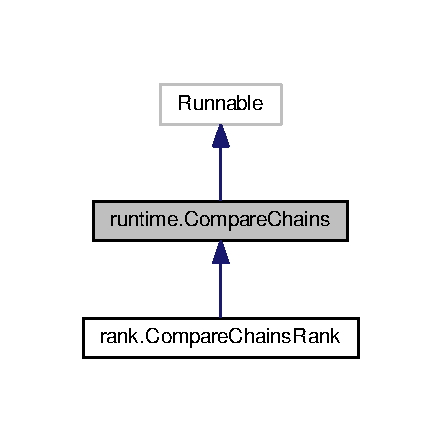
\includegraphics[width=212pt]{classruntime_1_1_compare_chains__inherit__graph}
\end{center}
\end{figure}


Collaboration diagram for runtime.\+Compare\+Chains\+:\nopagebreak
\begin{figure}[H]
\begin{center}
\leavevmode
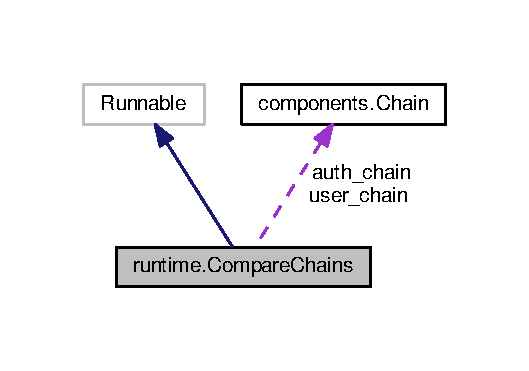
\includegraphics[width=254pt]{classruntime_1_1_compare_chains__coll__graph}
\end{center}
\end{figure}
\subsection*{Public Member Functions}
\begin{DoxyCompactItemize}
\item 
\hyperlink{classruntime_1_1_compare_chains_ae471eeb5d3db8b8e48784d86d5a14a44}{Compare\+Chains} (\hyperlink{classcomponents_1_1_chain}{Chain} \hyperlink{classruntime_1_1_compare_chains_ab222c09ed48638554987292979ede005}{user\+\_\+chain}, \hyperlink{classcomponents_1_1_chain}{Chain} \hyperlink{classruntime_1_1_compare_chains_ac78b36bc65a64fd14906685e6d9410a9}{auth\+\_\+chain})
\begin{DoxyCompactList}\small\item\em will need to make copies of the chains passed in so they do not get updated by something else during the comparason \end{DoxyCompactList}\item 
void \hyperlink{classruntime_1_1_compare_chains_aafa4a766a30bbbb6e205114a699d8158}{run} ()
\begin{DoxyCompactList}\small\item\em compare user\+\_\+chain and auth\+\_\+chain and choose what to do with the result \end{DoxyCompactList}\item 
double \hyperlink{classruntime_1_1_compare_chains_a684e7b6b0ea4f599a190866647acd144}{get\+\_\+auth\+\_\+probability} ()
\begin{DoxyCompactList}\small\item\em returns the probability with which the \end{DoxyCompactList}\item 
boolean \hyperlink{classruntime_1_1_compare_chains_af5dd0a0034121d92bbfac68adecec1c7}{get\+\_\+auth\+\_\+result} ()
\begin{DoxyCompactList}\small\item\em returns the result of the authentication. \end{DoxyCompactList}\item 
boolean \hyperlink{classruntime_1_1_compare_chains_a3e4a09371bcb8d006d646f9c58b5596c}{get\+\_\+auth\+\_\+complete} ()
\end{DoxyCompactItemize}
\subsection*{Protected Attributes}
\begin{DoxyCompactItemize}
\item 
volatile boolean \hyperlink{classruntime_1_1_compare_chains_a55fec8bf930fcd0c7ab835f14b85ac6d}{is\+\_\+authentic}
\item 
volatile boolean \hyperlink{classruntime_1_1_compare_chains_a506b689f300e16b70789ea87eef80387}{complete}
\item 
\hyperlink{classcomponents_1_1_chain}{Chain} \hyperlink{classruntime_1_1_compare_chains_ab222c09ed48638554987292979ede005}{user\+\_\+chain}
\item 
\hyperlink{classcomponents_1_1_chain}{Chain} \hyperlink{classruntime_1_1_compare_chains_ac78b36bc65a64fd14906685e6d9410a9}{auth\+\_\+chain}
\item 
volatile double \hyperlink{classruntime_1_1_compare_chains_a834721ac98cd7f0517344ab0c1afdf5c}{authentication\+\_\+probability}
\end{DoxyCompactItemize}


\subsection{Detailed Description}
Use the compare method of the Chain class to determine an authetnication probability between 0 and 1. 

This class was designed to allow for comparing chains to happen on a different thread. 

\subsection{Constructor \& Destructor Documentation}
\index{runtime\+::\+Compare\+Chains@{runtime\+::\+Compare\+Chains}!Compare\+Chains@{Compare\+Chains}}
\index{Compare\+Chains@{Compare\+Chains}!runtime\+::\+Compare\+Chains@{runtime\+::\+Compare\+Chains}}
\subsubsection[{\texorpdfstring{Compare\+Chains(\+Chain user\+\_\+chain, Chain auth\+\_\+chain)}{CompareChains(Chain user_chain, Chain auth_chain)}}]{\setlength{\rightskip}{0pt plus 5cm}runtime.\+Compare\+Chains.\+Compare\+Chains (
\begin{DoxyParamCaption}
\item[{{\bf Chain}}]{user\+\_\+chain, }
\item[{{\bf Chain}}]{auth\+\_\+chain}
\end{DoxyParamCaption}
)}\hypertarget{classruntime_1_1_compare_chains_ae471eeb5d3db8b8e48784d86d5a14a44}{}\label{classruntime_1_1_compare_chains_ae471eeb5d3db8b8e48784d86d5a14a44}


will need to make copies of the chains passed in so they do not get updated by something else during the comparason 



\subsection{Member Function Documentation}
\index{runtime\+::\+Compare\+Chains@{runtime\+::\+Compare\+Chains}!get\+\_\+auth\+\_\+complete@{get\+\_\+auth\+\_\+complete}}
\index{get\+\_\+auth\+\_\+complete@{get\+\_\+auth\+\_\+complete}!runtime\+::\+Compare\+Chains@{runtime\+::\+Compare\+Chains}}
\subsubsection[{\texorpdfstring{get\+\_\+auth\+\_\+complete()}{get_auth_complete()}}]{\setlength{\rightskip}{0pt plus 5cm}boolean runtime.\+Compare\+Chains.\+get\+\_\+auth\+\_\+complete (
\begin{DoxyParamCaption}
{}
\end{DoxyParamCaption}
)}\hypertarget{classruntime_1_1_compare_chains_a3e4a09371bcb8d006d646f9c58b5596c}{}\label{classruntime_1_1_compare_chains_a3e4a09371bcb8d006d646f9c58b5596c}


Here is the caller graph for this function\+:\nopagebreak
\begin{figure}[H]
\begin{center}
\leavevmode
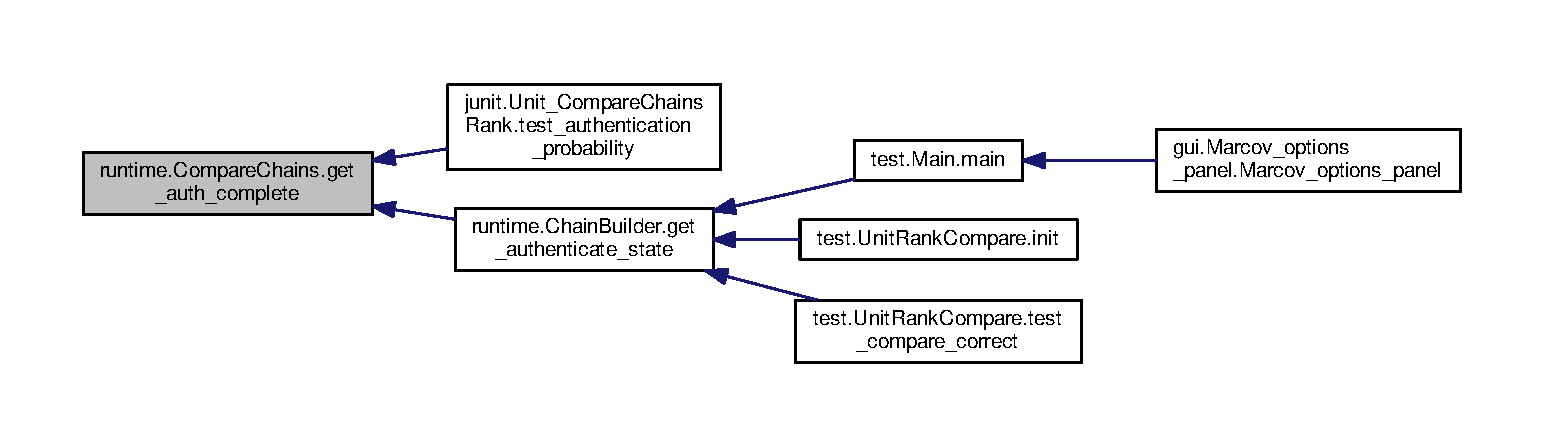
\includegraphics[width=350pt]{classruntime_1_1_compare_chains_a3e4a09371bcb8d006d646f9c58b5596c_icgraph}
\end{center}
\end{figure}


\index{runtime\+::\+Compare\+Chains@{runtime\+::\+Compare\+Chains}!get\+\_\+auth\+\_\+probability@{get\+\_\+auth\+\_\+probability}}
\index{get\+\_\+auth\+\_\+probability@{get\+\_\+auth\+\_\+probability}!runtime\+::\+Compare\+Chains@{runtime\+::\+Compare\+Chains}}
\subsubsection[{\texorpdfstring{get\+\_\+auth\+\_\+probability()}{get_auth_probability()}}]{\setlength{\rightskip}{0pt plus 5cm}double runtime.\+Compare\+Chains.\+get\+\_\+auth\+\_\+probability (
\begin{DoxyParamCaption}
{}
\end{DoxyParamCaption}
)}\hypertarget{classruntime_1_1_compare_chains_a684e7b6b0ea4f599a190866647acd144}{}\label{classruntime_1_1_compare_chains_a684e7b6b0ea4f599a190866647acd144}


returns the probability with which the 



Here is the caller graph for this function\+:\nopagebreak
\begin{figure}[H]
\begin{center}
\leavevmode
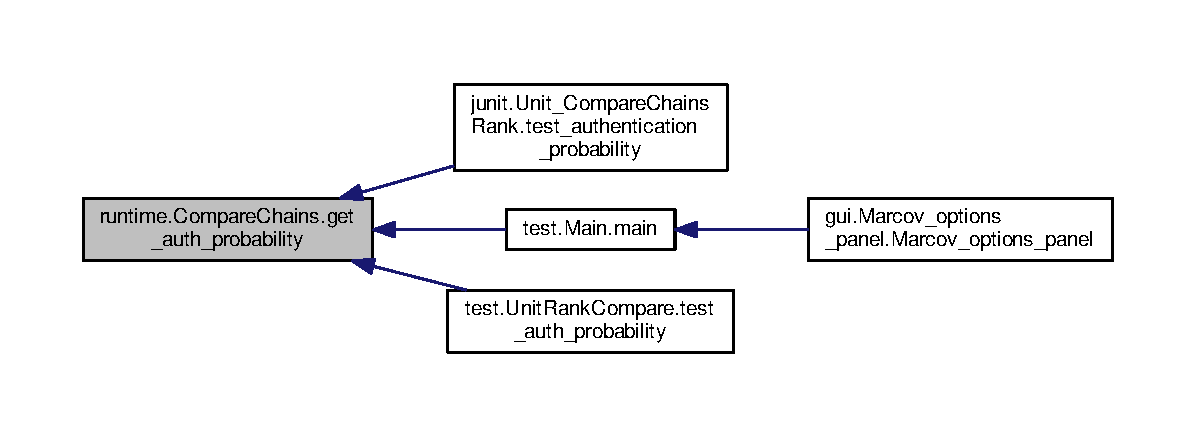
\includegraphics[width=350pt]{classruntime_1_1_compare_chains_a684e7b6b0ea4f599a190866647acd144_icgraph}
\end{center}
\end{figure}


\index{runtime\+::\+Compare\+Chains@{runtime\+::\+Compare\+Chains}!get\+\_\+auth\+\_\+result@{get\+\_\+auth\+\_\+result}}
\index{get\+\_\+auth\+\_\+result@{get\+\_\+auth\+\_\+result}!runtime\+::\+Compare\+Chains@{runtime\+::\+Compare\+Chains}}
\subsubsection[{\texorpdfstring{get\+\_\+auth\+\_\+result()}{get_auth_result()}}]{\setlength{\rightskip}{0pt plus 5cm}boolean runtime.\+Compare\+Chains.\+get\+\_\+auth\+\_\+result (
\begin{DoxyParamCaption}
{}
\end{DoxyParamCaption}
)}\hypertarget{classruntime_1_1_compare_chains_af5dd0a0034121d92bbfac68adecec1c7}{}\label{classruntime_1_1_compare_chains_af5dd0a0034121d92bbfac68adecec1c7}


returns the result of the authentication. 

This method does not provide any guarentees that the compairason has finsihed yet. If the compairason has not yet finished it will return false; 

Here is the caller graph for this function\+:\nopagebreak
\begin{figure}[H]
\begin{center}
\leavevmode
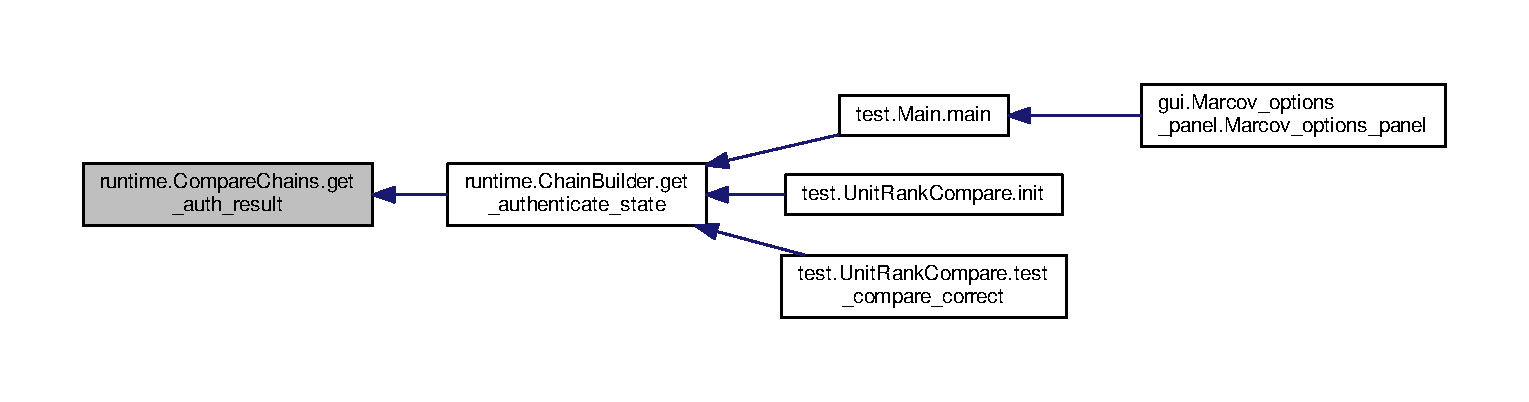
\includegraphics[width=350pt]{classruntime_1_1_compare_chains_af5dd0a0034121d92bbfac68adecec1c7_icgraph}
\end{center}
\end{figure}


\index{runtime\+::\+Compare\+Chains@{runtime\+::\+Compare\+Chains}!run@{run}}
\index{run@{run}!runtime\+::\+Compare\+Chains@{runtime\+::\+Compare\+Chains}}
\subsubsection[{\texorpdfstring{run()}{run()}}]{\setlength{\rightskip}{0pt plus 5cm}void runtime.\+Compare\+Chains.\+run (
\begin{DoxyParamCaption}
{}
\end{DoxyParamCaption}
)}\hypertarget{classruntime_1_1_compare_chains_aafa4a766a30bbbb6e205114a699d8158}{}\label{classruntime_1_1_compare_chains_aafa4a766a30bbbb6e205114a699d8158}


compare user\+\_\+chain and auth\+\_\+chain and choose what to do with the result 

perform the comparison now that the values are cached in the Chain\textquotesingle{}s 

Here is the call graph for this function\+:\nopagebreak
\begin{figure}[H]
\begin{center}
\leavevmode
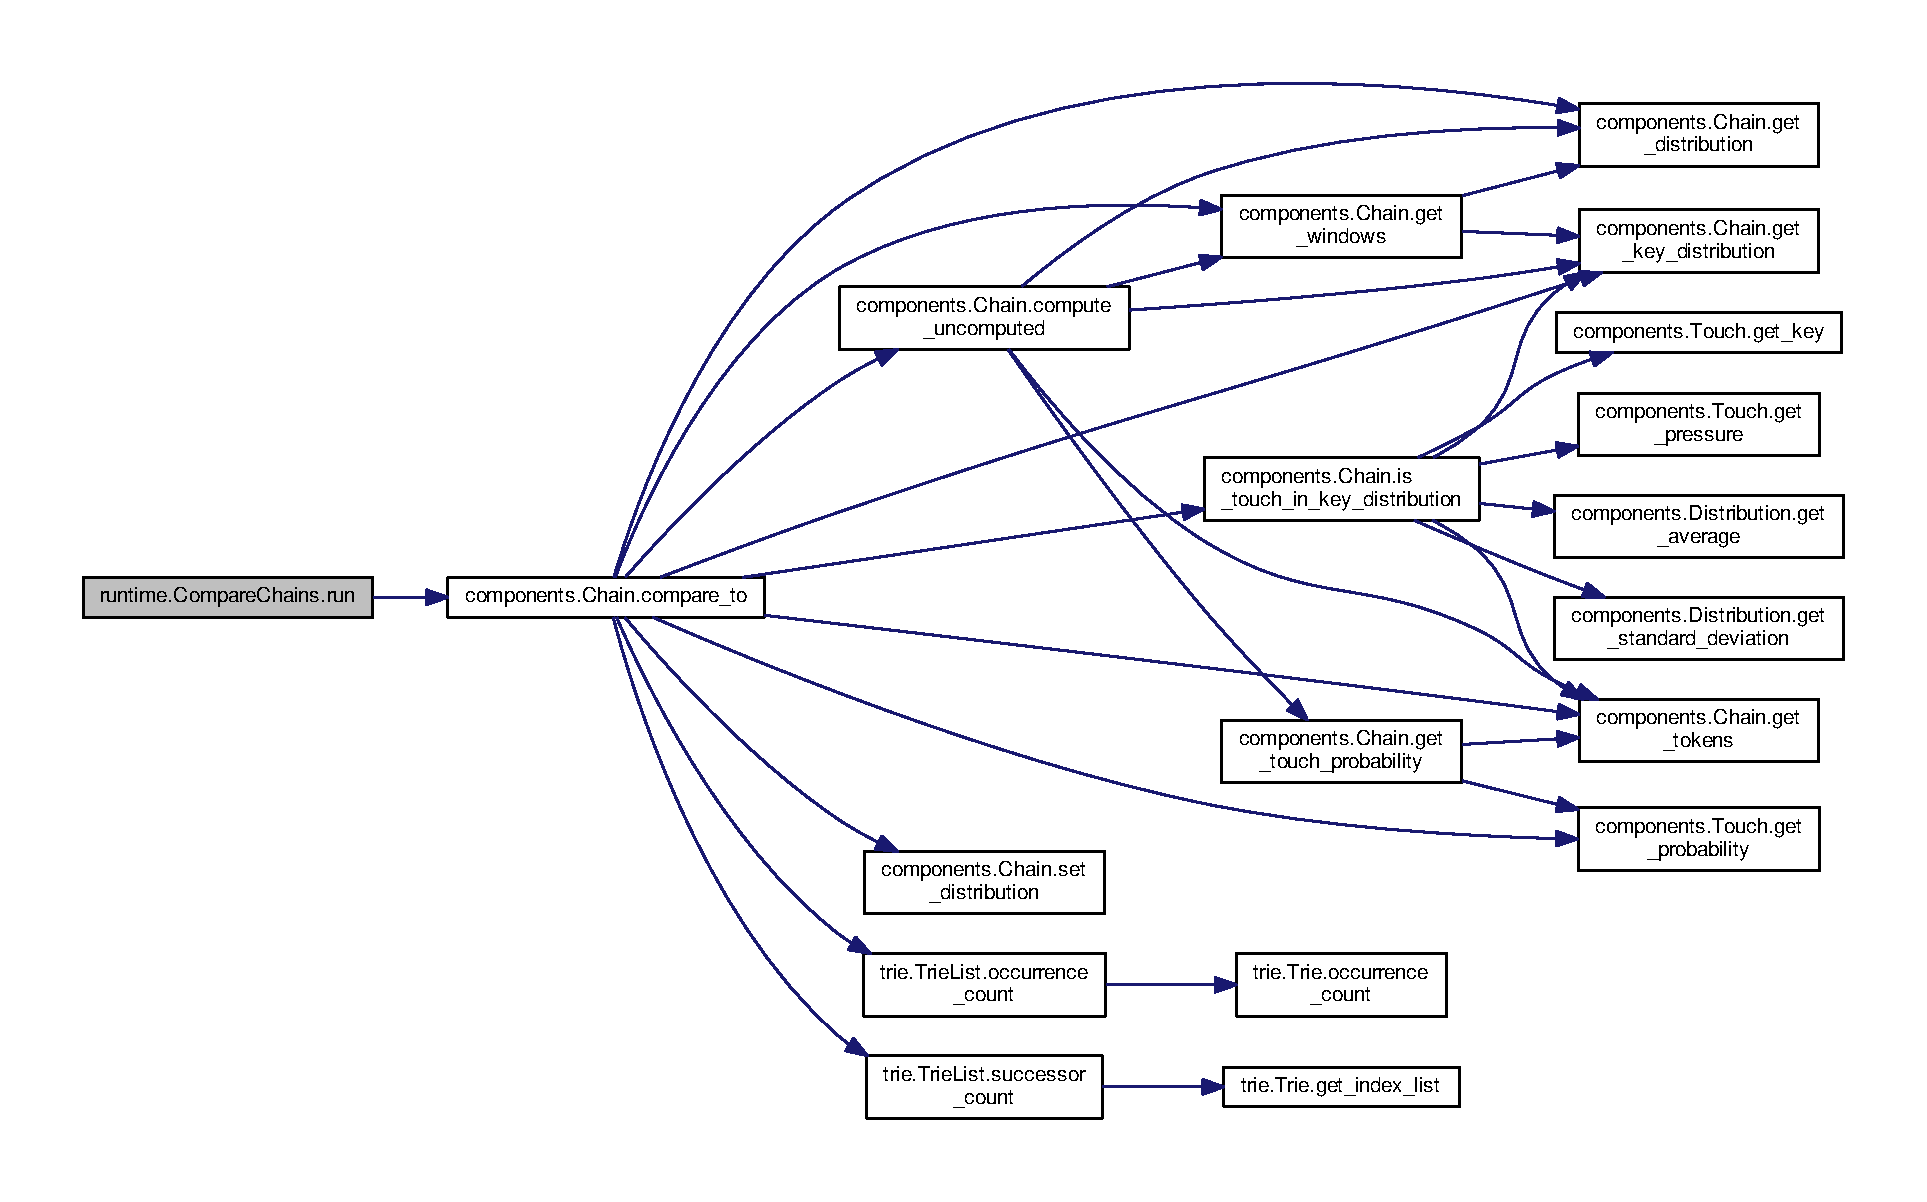
\includegraphics[width=350pt]{classruntime_1_1_compare_chains_aafa4a766a30bbbb6e205114a699d8158_cgraph}
\end{center}
\end{figure}




\subsection{Member Data Documentation}
\index{runtime\+::\+Compare\+Chains@{runtime\+::\+Compare\+Chains}!auth\+\_\+chain@{auth\+\_\+chain}}
\index{auth\+\_\+chain@{auth\+\_\+chain}!runtime\+::\+Compare\+Chains@{runtime\+::\+Compare\+Chains}}
\subsubsection[{\texorpdfstring{auth\+\_\+chain}{auth_chain}}]{\setlength{\rightskip}{0pt plus 5cm}{\bf Chain} runtime.\+Compare\+Chains.\+auth\+\_\+chain\hspace{0.3cm}{\ttfamily [protected]}}\hypertarget{classruntime_1_1_compare_chains_ac78b36bc65a64fd14906685e6d9410a9}{}\label{classruntime_1_1_compare_chains_ac78b36bc65a64fd14906685e6d9410a9}
\index{runtime\+::\+Compare\+Chains@{runtime\+::\+Compare\+Chains}!authentication\+\_\+probability@{authentication\+\_\+probability}}
\index{authentication\+\_\+probability@{authentication\+\_\+probability}!runtime\+::\+Compare\+Chains@{runtime\+::\+Compare\+Chains}}
\subsubsection[{\texorpdfstring{authentication\+\_\+probability}{authentication_probability}}]{\setlength{\rightskip}{0pt plus 5cm}volatile double runtime.\+Compare\+Chains.\+authentication\+\_\+probability\hspace{0.3cm}{\ttfamily [protected]}}\hypertarget{classruntime_1_1_compare_chains_a834721ac98cd7f0517344ab0c1afdf5c}{}\label{classruntime_1_1_compare_chains_a834721ac98cd7f0517344ab0c1afdf5c}
\index{runtime\+::\+Compare\+Chains@{runtime\+::\+Compare\+Chains}!complete@{complete}}
\index{complete@{complete}!runtime\+::\+Compare\+Chains@{runtime\+::\+Compare\+Chains}}
\subsubsection[{\texorpdfstring{complete}{complete}}]{\setlength{\rightskip}{0pt plus 5cm}volatile boolean runtime.\+Compare\+Chains.\+complete\hspace{0.3cm}{\ttfamily [protected]}}\hypertarget{classruntime_1_1_compare_chains_a506b689f300e16b70789ea87eef80387}{}\label{classruntime_1_1_compare_chains_a506b689f300e16b70789ea87eef80387}
\index{runtime\+::\+Compare\+Chains@{runtime\+::\+Compare\+Chains}!is\+\_\+authentic@{is\+\_\+authentic}}
\index{is\+\_\+authentic@{is\+\_\+authentic}!runtime\+::\+Compare\+Chains@{runtime\+::\+Compare\+Chains}}
\subsubsection[{\texorpdfstring{is\+\_\+authentic}{is_authentic}}]{\setlength{\rightskip}{0pt plus 5cm}volatile boolean runtime.\+Compare\+Chains.\+is\+\_\+authentic\hspace{0.3cm}{\ttfamily [protected]}}\hypertarget{classruntime_1_1_compare_chains_a55fec8bf930fcd0c7ab835f14b85ac6d}{}\label{classruntime_1_1_compare_chains_a55fec8bf930fcd0c7ab835f14b85ac6d}
\index{runtime\+::\+Compare\+Chains@{runtime\+::\+Compare\+Chains}!user\+\_\+chain@{user\+\_\+chain}}
\index{user\+\_\+chain@{user\+\_\+chain}!runtime\+::\+Compare\+Chains@{runtime\+::\+Compare\+Chains}}
\subsubsection[{\texorpdfstring{user\+\_\+chain}{user_chain}}]{\setlength{\rightskip}{0pt plus 5cm}{\bf Chain} runtime.\+Compare\+Chains.\+user\+\_\+chain\hspace{0.3cm}{\ttfamily [protected]}}\hypertarget{classruntime_1_1_compare_chains_ab222c09ed48638554987292979ede005}{}\label{classruntime_1_1_compare_chains_ab222c09ed48638554987292979ede005}


The documentation for this class was generated from the following file\+:\begin{DoxyCompactItemize}
\item 
/home/element/\+P\+U\+F/\+Keyboard/java\+\_\+scripts/java\+\_\+marcov\+\_\+model/src/runtime/\hyperlink{_compare_chains_8java}{Compare\+Chains.\+java}\end{DoxyCompactItemize}

\hypertarget{classrank_1_1_compare_chains_rank}{}\section{rank.\+Compare\+Chains\+Rank Class Reference}
\label{classrank_1_1_compare_chains_rank}\index{rank.\+Compare\+Chains\+Rank@{rank.\+Compare\+Chains\+Rank}}


Use Page\+Rank algorithm (library) to compare chains.  




Inheritance diagram for rank.\+Compare\+Chains\+Rank\+:
\nopagebreak
\begin{figure}[H]
\begin{center}
\leavevmode
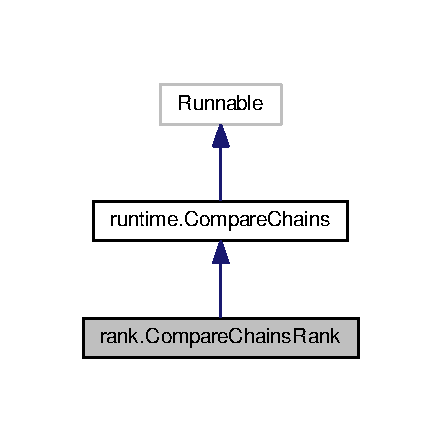
\includegraphics[width=212pt]{classrank_1_1_compare_chains_rank__inherit__graph}
\end{center}
\end{figure}


Collaboration diagram for rank.\+Compare\+Chains\+Rank\+:
\nopagebreak
\begin{figure}[H]
\begin{center}
\leavevmode
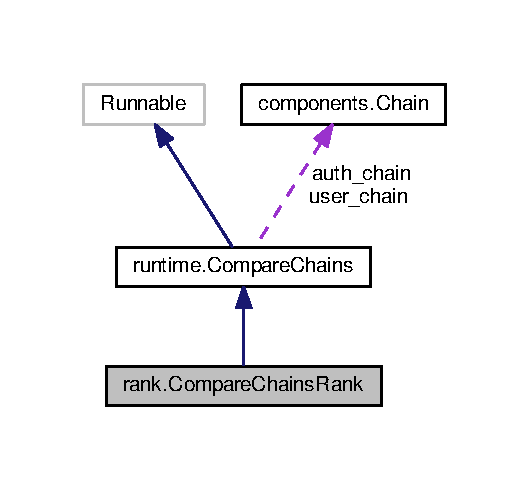
\includegraphics[width=254pt]{classrank_1_1_compare_chains_rank__coll__graph}
\end{center}
\end{figure}
\subsection*{Public Member Functions}
\begin{DoxyCompactItemize}
\item 
\hyperlink{classrank_1_1_compare_chains_rank_ac03c8c50833f034c8d0e1f8de219559e}{Compare\+Chains\+Rank} (\hyperlink{classcomponents_1_1_chain}{Chain} \hyperlink{classruntime_1_1_compare_chains_ab222c09ed48638554987292979ede005}{user\+\_\+chain}, \hyperlink{classcomponents_1_1_chain}{Chain} \hyperlink{classruntime_1_1_compare_chains_ac78b36bc65a64fd14906685e6d9410a9}{auth\+\_\+chain})
\item 
void \hyperlink{classrank_1_1_compare_chains_rank_a72680cae41f481bfe37011051c2e9419}{run} ()
\begin{DoxyCompactList}\small\item\em overrides the run method to implement the authentication with a page-\/rank style algorithm. \end{DoxyCompactList}\end{DoxyCompactItemize}
\subsection*{Additional Inherited Members}


\subsection{Detailed Description}
Use Page\+Rank algorithm (library) to compare chains. 

Provides an implementation of Compare\+Chains which can be used in place of the chain compairason implemented in the Chain class.

N\+O\+TE\+: this is still a work in progress and does not have very good results yet. 

\subsection{Constructor \& Destructor Documentation}
\index{rank\+::\+Compare\+Chains\+Rank@{rank\+::\+Compare\+Chains\+Rank}!Compare\+Chains\+Rank@{Compare\+Chains\+Rank}}
\index{Compare\+Chains\+Rank@{Compare\+Chains\+Rank}!rank\+::\+Compare\+Chains\+Rank@{rank\+::\+Compare\+Chains\+Rank}}
\subsubsection[{\texorpdfstring{Compare\+Chains\+Rank(\+Chain user\+\_\+chain, Chain auth\+\_\+chain)}{CompareChainsRank(Chain user_chain, Chain auth_chain)}}]{\setlength{\rightskip}{0pt plus 5cm}rank.\+Compare\+Chains\+Rank.\+Compare\+Chains\+Rank (
\begin{DoxyParamCaption}
\item[{{\bf Chain}}]{user\+\_\+chain, }
\item[{{\bf Chain}}]{auth\+\_\+chain}
\end{DoxyParamCaption}
)}\hypertarget{classrank_1_1_compare_chains_rank_ac03c8c50833f034c8d0e1f8de219559e}{}\label{classrank_1_1_compare_chains_rank_ac03c8c50833f034c8d0e1f8de219559e}


\subsection{Member Function Documentation}
\index{rank\+::\+Compare\+Chains\+Rank@{rank\+::\+Compare\+Chains\+Rank}!run@{run}}
\index{run@{run}!rank\+::\+Compare\+Chains\+Rank@{rank\+::\+Compare\+Chains\+Rank}}
\subsubsection[{\texorpdfstring{run()}{run()}}]{\setlength{\rightskip}{0pt plus 5cm}void rank.\+Compare\+Chains\+Rank.\+run (
\begin{DoxyParamCaption}
{}
\end{DoxyParamCaption}
)}\hypertarget{classrank_1_1_compare_chains_rank_a72680cae41f481bfe37011051c2e9419}{}\label{classrank_1_1_compare_chains_rank_a72680cae41f481bfe37011051c2e9419}


overrides the run method to implement the authentication with a page-\/rank style algorithm. 



Here is the call graph for this function\+:\nopagebreak
\begin{figure}[H]
\begin{center}
\leavevmode
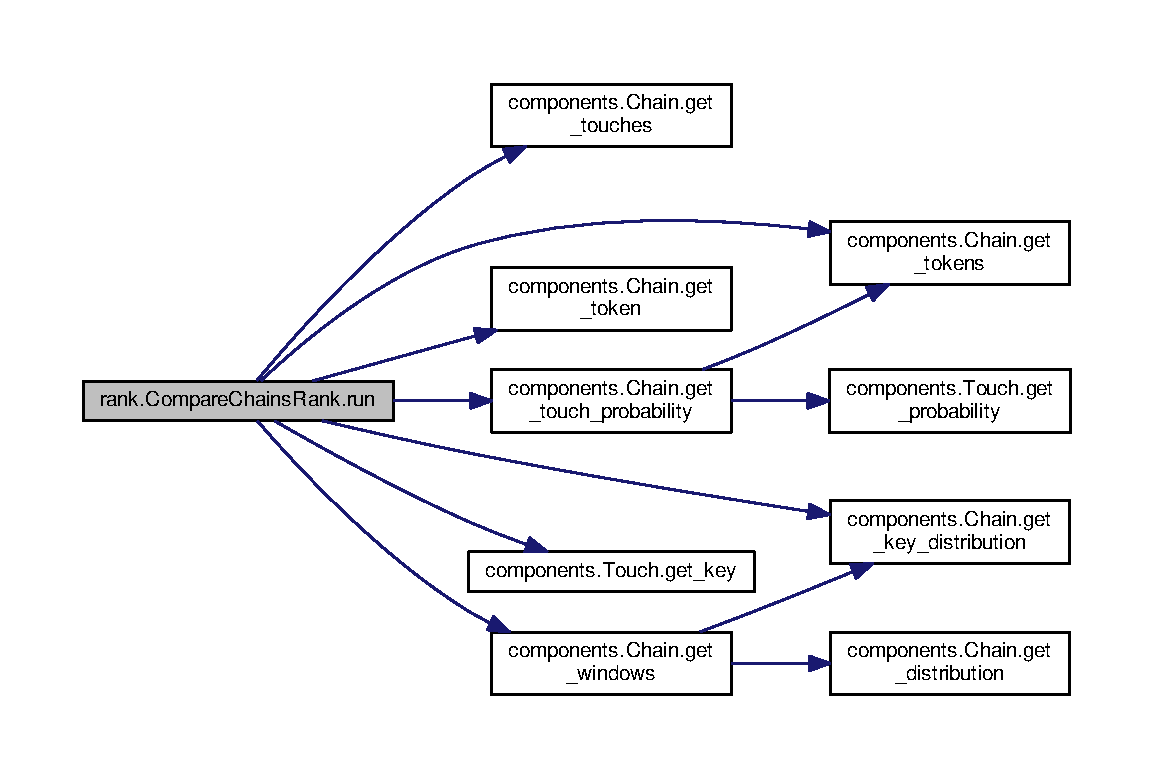
\includegraphics[width=350pt]{classrank_1_1_compare_chains_rank_a72680cae41f481bfe37011051c2e9419_cgraph}
\end{center}
\end{figure}




The documentation for this class was generated from the following file\+:\begin{DoxyCompactItemize}
\item 
/home/element/\+P\+U\+F/\+Keyboard/java\+\_\+scripts/java\+\_\+marcov\+\_\+model/src/rank/\hyperlink{_compare_chains_rank_8java}{Compare\+Chains\+Rank.\+java}\end{DoxyCompactItemize}

\hypertarget{enumruntime_1_1_chain_builder_1_1_compare_method}{}\section{runtime.\+Chain\+Builder.\+Compare\+Method Enum Reference}
\label{enumruntime_1_1_chain_builder_1_1_compare_method}\index{runtime.\+Chain\+Builder.\+Compare\+Method@{runtime.\+Chain\+Builder.\+Compare\+Method}}
\subsection*{Public Attributes}
\begin{DoxyCompactItemize}
\item 
\hyperlink{enumruntime_1_1_chain_builder_1_1_compare_method_a98895b1f0e70abffdabedbbac9a45bd4}{P\+R\+O\+B\+A\+B\+I\+L\+I\+T\+Y\+\_\+\+V\+E\+C\+T\+O\+R\+\_\+\+D\+I\+F\+F\+E\+R\+A\+N\+CE}
\end{DoxyCompactItemize}


\subsection{Member Data Documentation}
\index{runtime\+::\+Chain\+Builder\+::\+Compare\+Method@{runtime\+::\+Chain\+Builder\+::\+Compare\+Method}!P\+R\+O\+B\+A\+B\+I\+L\+I\+T\+Y\+\_\+\+V\+E\+C\+T\+O\+R\+\_\+\+D\+I\+F\+F\+E\+R\+A\+N\+CE@{P\+R\+O\+B\+A\+B\+I\+L\+I\+T\+Y\+\_\+\+V\+E\+C\+T\+O\+R\+\_\+\+D\+I\+F\+F\+E\+R\+A\+N\+CE}}
\index{P\+R\+O\+B\+A\+B\+I\+L\+I\+T\+Y\+\_\+\+V\+E\+C\+T\+O\+R\+\_\+\+D\+I\+F\+F\+E\+R\+A\+N\+CE@{P\+R\+O\+B\+A\+B\+I\+L\+I\+T\+Y\+\_\+\+V\+E\+C\+T\+O\+R\+\_\+\+D\+I\+F\+F\+E\+R\+A\+N\+CE}!runtime\+::\+Chain\+Builder\+::\+Compare\+Method@{runtime\+::\+Chain\+Builder\+::\+Compare\+Method}}
\subsubsection[{\texorpdfstring{P\+R\+O\+B\+A\+B\+I\+L\+I\+T\+Y\+\_\+\+V\+E\+C\+T\+O\+R\+\_\+\+D\+I\+F\+F\+E\+R\+A\+N\+CE}{PROBABILITY_VECTOR_DIFFERANCE}}]{\setlength{\rightskip}{0pt plus 5cm}runtime.\+Chain\+Builder.\+Compare\+Method.\+P\+R\+O\+B\+A\+B\+I\+L\+I\+T\+Y\+\_\+\+V\+E\+C\+T\+O\+R\+\_\+\+D\+I\+F\+F\+E\+R\+A\+N\+CE}\hypertarget{enumruntime_1_1_chain_builder_1_1_compare_method_a98895b1f0e70abffdabedbbac9a45bd4}{}\label{enumruntime_1_1_chain_builder_1_1_compare_method_a98895b1f0e70abffdabedbbac9a45bd4}


The documentation for this enum was generated from the following file\+:\begin{DoxyCompactItemize}
\item 
/home/element/\+P\+U\+F/\+Keyboard/java\+\_\+scripts/java\+\_\+marcov\+\_\+model/src/runtime/\hyperlink{_chain_builder_8java}{Chain\+Builder.\+java}\end{DoxyCompactItemize}

\hypertarget{classrank_1_1_complete_probability}{}\section{rank.\+Complete\+Probability Class Reference}
\label{classrank_1_1_complete_probability}\index{rank.\+Complete\+Probability@{rank.\+Complete\+Probability}}


This class computes probability in a different way from what is contained in the Chain class.  


\subsection*{Public Member Functions}
\begin{DoxyCompactItemize}
\item 
\hyperlink{classrank_1_1_complete_probability_a0c57b2805fa39cdc190edbba9ea5a86c}{Complete\+Probability} (\hyperlink{classcomponents_1_1_chain}{Chain} chain)
\item 
\hyperlink{classcomponents_1_1_chain}{Chain} \hyperlink{classrank_1_1_complete_probability_a1507b6695918da300c0130ccdc218900}{compute\+\_\+probability} ()
\begin{DoxyCompactList}\small\item\em make a replica of the chain with a window size of 1 and compute the probability. \end{DoxyCompactList}\end{DoxyCompactItemize}


\subsection{Detailed Description}
This class computes probability in a different way from what is contained in the Chain class. 

This class looks at all of the touches to try to determine the probability that from any given touch, it transitions to another.

this is similar to having a window size of 1?

\begin{DoxyAuthor}{Author}
element 
\end{DoxyAuthor}


\subsection{Constructor \& Destructor Documentation}
\index{rank\+::\+Complete\+Probability@{rank\+::\+Complete\+Probability}!Complete\+Probability@{Complete\+Probability}}
\index{Complete\+Probability@{Complete\+Probability}!rank\+::\+Complete\+Probability@{rank\+::\+Complete\+Probability}}
\subsubsection[{\texorpdfstring{Complete\+Probability(\+Chain chain)}{CompleteProbability(Chain chain)}}]{\setlength{\rightskip}{0pt plus 5cm}rank.\+Complete\+Probability.\+Complete\+Probability (
\begin{DoxyParamCaption}
\item[{{\bf Chain}}]{chain}
\end{DoxyParamCaption}
)}\hypertarget{classrank_1_1_complete_probability_a0c57b2805fa39cdc190edbba9ea5a86c}{}\label{classrank_1_1_complete_probability_a0c57b2805fa39cdc190edbba9ea5a86c}


\subsection{Member Function Documentation}
\index{rank\+::\+Complete\+Probability@{rank\+::\+Complete\+Probability}!compute\+\_\+probability@{compute\+\_\+probability}}
\index{compute\+\_\+probability@{compute\+\_\+probability}!rank\+::\+Complete\+Probability@{rank\+::\+Complete\+Probability}}
\subsubsection[{\texorpdfstring{compute\+\_\+probability()}{compute_probability()}}]{\setlength{\rightskip}{0pt plus 5cm}{\bf Chain} rank.\+Complete\+Probability.\+compute\+\_\+probability (
\begin{DoxyParamCaption}
{}
\end{DoxyParamCaption}
)}\hypertarget{classrank_1_1_complete_probability_a1507b6695918da300c0130ccdc218900}{}\label{classrank_1_1_complete_probability_a1507b6695918da300c0130ccdc218900}


make a replica of the chain with a window size of 1 and compute the probability. 

\begin{DoxyReturn}{Returns}
replica chain 
\end{DoxyReturn}


Here is the call graph for this function\+:\nopagebreak
\begin{figure}[H]
\begin{center}
\leavevmode
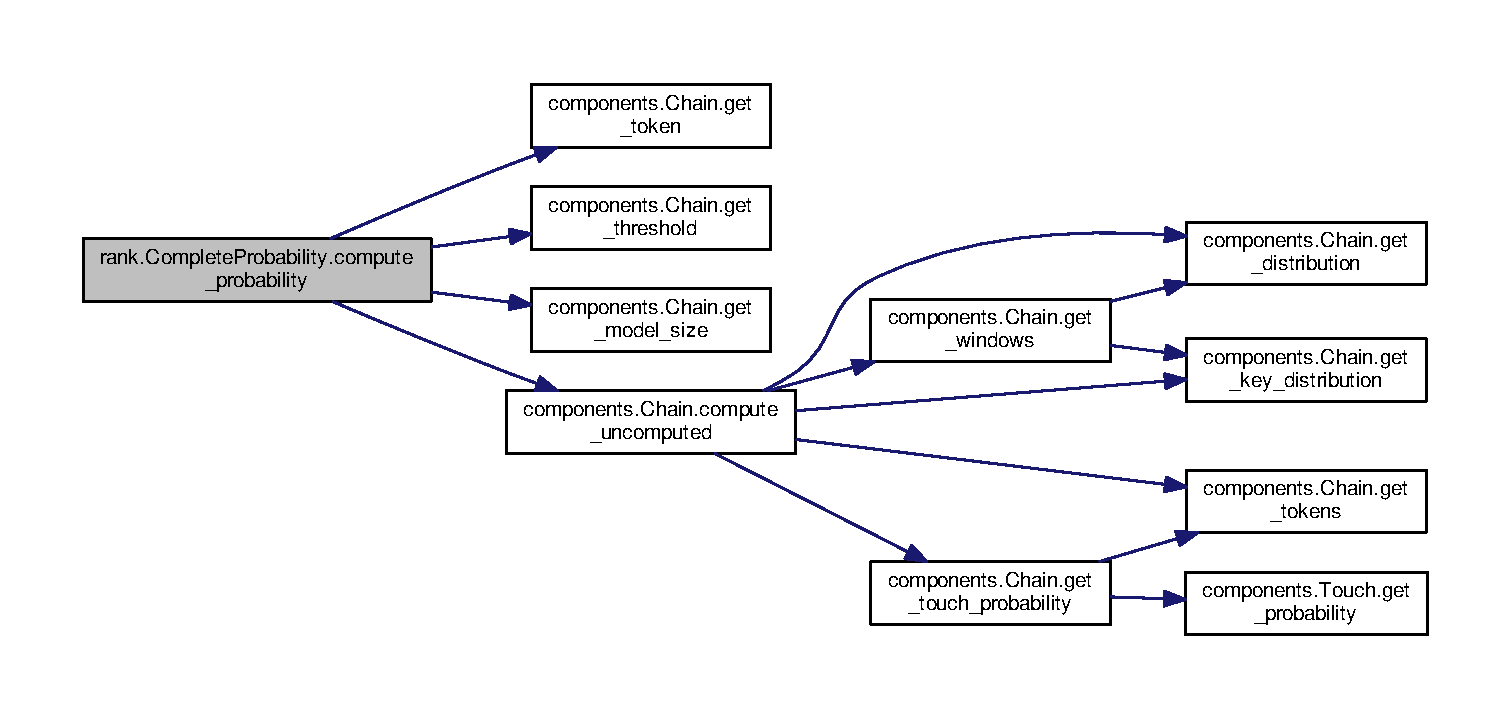
\includegraphics[width=350pt]{classrank_1_1_complete_probability_a1507b6695918da300c0130ccdc218900_cgraph}
\end{center}
\end{figure}




Here is the caller graph for this function\+:\nopagebreak
\begin{figure}[H]
\begin{center}
\leavevmode
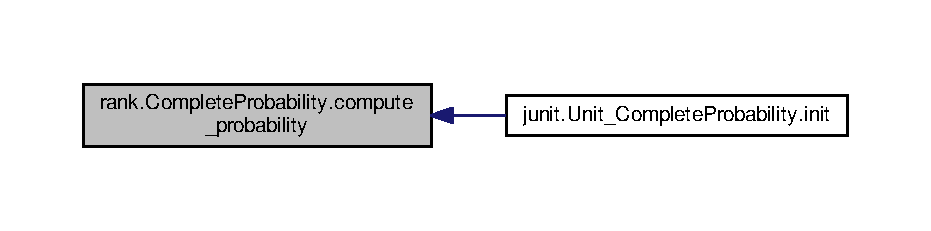
\includegraphics[width=350pt]{classrank_1_1_complete_probability_a1507b6695918da300c0130ccdc218900_icgraph}
\end{center}
\end{figure}




The documentation for this class was generated from the following file\+:\begin{DoxyCompactItemize}
\item 
/home/element/\+P\+U\+F/\+Keyboard/java\+\_\+scripts/java\+\_\+marcov\+\_\+model/src/rank/\hyperlink{_complete_probability_8java}{Complete\+Probability.\+java}\end{DoxyCompactItemize}

\hypertarget{enumruntime_1_1_operation__thread_1_1_computation}{}\section{runtime.\+Operation\+\_\+thread.\+Computation Enum Reference}
\label{enumruntime_1_1_operation__thread_1_1_computation}\index{runtime.\+Operation\+\_\+thread.\+Computation@{runtime.\+Operation\+\_\+thread.\+Computation}}
\subsection*{Public Attributes}
\begin{DoxyCompactItemize}
\item 
\hyperlink{enumruntime_1_1_operation__thread_1_1_computation_a6381fe8b51eee311dff627d315fefbfd}{D\+I\+S\+T\+R\+I\+B\+U\+T\+I\+ON}
\item 
\hyperlink{enumruntime_1_1_operation__thread_1_1_computation_a8235775e9276cd32feb00cd4ca2e0a35}{K\+E\+Y\+\_\+\+D\+I\+S\+T\+R\+I\+B\+U\+T\+I\+ON}
\item 
\hyperlink{enumruntime_1_1_operation__thread_1_1_computation_aa6eb3addd3d9b5c6002a65ad02b48558}{W\+I\+N\+D\+OW}
\item 
\hyperlink{enumruntime_1_1_operation__thread_1_1_computation_a67a1e69588a63abbde225f5a249623c5}{T\+O\+K\+EN}
\item 
\hyperlink{enumruntime_1_1_operation__thread_1_1_computation_abe18ce6bfa0196cd62df7cb6fb7a9427}{P\+R\+O\+B\+A\+B\+I\+L\+I\+TY}
\end{DoxyCompactItemize}


\subsection{Member Data Documentation}
\index{runtime\+::\+Operation\+\_\+thread\+::\+Computation@{runtime\+::\+Operation\+\_\+thread\+::\+Computation}!D\+I\+S\+T\+R\+I\+B\+U\+T\+I\+ON@{D\+I\+S\+T\+R\+I\+B\+U\+T\+I\+ON}}
\index{D\+I\+S\+T\+R\+I\+B\+U\+T\+I\+ON@{D\+I\+S\+T\+R\+I\+B\+U\+T\+I\+ON}!runtime\+::\+Operation\+\_\+thread\+::\+Computation@{runtime\+::\+Operation\+\_\+thread\+::\+Computation}}
\subsubsection[{\texorpdfstring{D\+I\+S\+T\+R\+I\+B\+U\+T\+I\+ON}{DISTRIBUTION}}]{\setlength{\rightskip}{0pt plus 5cm}runtime.\+Operation\+\_\+thread.\+Computation.\+D\+I\+S\+T\+R\+I\+B\+U\+T\+I\+ON}\hypertarget{enumruntime_1_1_operation__thread_1_1_computation_a6381fe8b51eee311dff627d315fefbfd}{}\label{enumruntime_1_1_operation__thread_1_1_computation_a6381fe8b51eee311dff627d315fefbfd}
\index{runtime\+::\+Operation\+\_\+thread\+::\+Computation@{runtime\+::\+Operation\+\_\+thread\+::\+Computation}!K\+E\+Y\+\_\+\+D\+I\+S\+T\+R\+I\+B\+U\+T\+I\+ON@{K\+E\+Y\+\_\+\+D\+I\+S\+T\+R\+I\+B\+U\+T\+I\+ON}}
\index{K\+E\+Y\+\_\+\+D\+I\+S\+T\+R\+I\+B\+U\+T\+I\+ON@{K\+E\+Y\+\_\+\+D\+I\+S\+T\+R\+I\+B\+U\+T\+I\+ON}!runtime\+::\+Operation\+\_\+thread\+::\+Computation@{runtime\+::\+Operation\+\_\+thread\+::\+Computation}}
\subsubsection[{\texorpdfstring{K\+E\+Y\+\_\+\+D\+I\+S\+T\+R\+I\+B\+U\+T\+I\+ON}{KEY_DISTRIBUTION}}]{\setlength{\rightskip}{0pt plus 5cm}runtime.\+Operation\+\_\+thread.\+Computation.\+K\+E\+Y\+\_\+\+D\+I\+S\+T\+R\+I\+B\+U\+T\+I\+ON}\hypertarget{enumruntime_1_1_operation__thread_1_1_computation_a8235775e9276cd32feb00cd4ca2e0a35}{}\label{enumruntime_1_1_operation__thread_1_1_computation_a8235775e9276cd32feb00cd4ca2e0a35}
\index{runtime\+::\+Operation\+\_\+thread\+::\+Computation@{runtime\+::\+Operation\+\_\+thread\+::\+Computation}!P\+R\+O\+B\+A\+B\+I\+L\+I\+TY@{P\+R\+O\+B\+A\+B\+I\+L\+I\+TY}}
\index{P\+R\+O\+B\+A\+B\+I\+L\+I\+TY@{P\+R\+O\+B\+A\+B\+I\+L\+I\+TY}!runtime\+::\+Operation\+\_\+thread\+::\+Computation@{runtime\+::\+Operation\+\_\+thread\+::\+Computation}}
\subsubsection[{\texorpdfstring{P\+R\+O\+B\+A\+B\+I\+L\+I\+TY}{PROBABILITY}}]{\setlength{\rightskip}{0pt plus 5cm}runtime.\+Operation\+\_\+thread.\+Computation.\+P\+R\+O\+B\+A\+B\+I\+L\+I\+TY}\hypertarget{enumruntime_1_1_operation__thread_1_1_computation_abe18ce6bfa0196cd62df7cb6fb7a9427}{}\label{enumruntime_1_1_operation__thread_1_1_computation_abe18ce6bfa0196cd62df7cb6fb7a9427}
\index{runtime\+::\+Operation\+\_\+thread\+::\+Computation@{runtime\+::\+Operation\+\_\+thread\+::\+Computation}!T\+O\+K\+EN@{T\+O\+K\+EN}}
\index{T\+O\+K\+EN@{T\+O\+K\+EN}!runtime\+::\+Operation\+\_\+thread\+::\+Computation@{runtime\+::\+Operation\+\_\+thread\+::\+Computation}}
\subsubsection[{\texorpdfstring{T\+O\+K\+EN}{TOKEN}}]{\setlength{\rightskip}{0pt plus 5cm}runtime.\+Operation\+\_\+thread.\+Computation.\+T\+O\+K\+EN}\hypertarget{enumruntime_1_1_operation__thread_1_1_computation_a67a1e69588a63abbde225f5a249623c5}{}\label{enumruntime_1_1_operation__thread_1_1_computation_a67a1e69588a63abbde225f5a249623c5}
\index{runtime\+::\+Operation\+\_\+thread\+::\+Computation@{runtime\+::\+Operation\+\_\+thread\+::\+Computation}!W\+I\+N\+D\+OW@{W\+I\+N\+D\+OW}}
\index{W\+I\+N\+D\+OW@{W\+I\+N\+D\+OW}!runtime\+::\+Operation\+\_\+thread\+::\+Computation@{runtime\+::\+Operation\+\_\+thread\+::\+Computation}}
\subsubsection[{\texorpdfstring{W\+I\+N\+D\+OW}{WINDOW}}]{\setlength{\rightskip}{0pt plus 5cm}runtime.\+Operation\+\_\+thread.\+Computation.\+W\+I\+N\+D\+OW}\hypertarget{enumruntime_1_1_operation__thread_1_1_computation_aa6eb3addd3d9b5c6002a65ad02b48558}{}\label{enumruntime_1_1_operation__thread_1_1_computation_aa6eb3addd3d9b5c6002a65ad02b48558}


The documentation for this enum was generated from the following file\+:\begin{DoxyCompactItemize}
\item 
/home/element/\+P\+U\+F/\+Keyboard/java\+\_\+scripts/java\+\_\+marcov\+\_\+model/src/runtime/\hyperlink{_operation__thread_8java}{Operation\+\_\+thread.\+java}\end{DoxyCompactItemize}

\hypertarget{enumtest_1_1_main_1_1_test_files_1_1_concentration}{}\section{test.\+Main.\+Test\+Files.\+Concentration Enum Reference}
\label{enumtest_1_1_main_1_1_test_files_1_1_concentration}\index{test.\+Main.\+Test\+Files.\+Concentration@{test.\+Main.\+Test\+Files.\+Concentration}}
\subsection*{Public Member Functions}
\begin{DoxyCompactItemize}
\item 
\hyperlink{enumtest_1_1_main_1_1_test_files_1_1_concentration_a8365a18de30b5d4538b2bc3a105ca652}{Concentration} (String description, int identifier, double value)
\item 
String \hyperlink{enumtest_1_1_main_1_1_test_files_1_1_concentration_a0669104e51effe316491287b5ce9366f}{to\+String} ()
\item 
int \hyperlink{enumtest_1_1_main_1_1_test_files_1_1_concentration_a45beb7f5967ebd747c9d325286f25125}{get\+\_\+identifier} ()
\item 
double \hyperlink{enumtest_1_1_main_1_1_test_files_1_1_concentration_aaae7c673fc7a17d505de14d962b16e59}{get\+\_\+value} ()
\end{DoxyCompactItemize}
\subsection*{Public Attributes}
\begin{DoxyCompactItemize}
\item 
\hyperlink{enumtest_1_1_main_1_1_test_files_1_1_concentration_a9de91ec8dd5ed01507aea649af87b0ed}{H\+I\+GH} =(\char`\"{}High, \mbox{[}std deviation\mbox{]}\char`\"{}, 0, 0)
\item 
\hyperlink{enumtest_1_1_main_1_1_test_files_1_1_concentration_aa63ada2a9617b0ac561c5ca3d0e31069}{M\+E\+D\+I\+UM} =(\char`\"{}Medium, \mbox{[}std deviation\mbox{]}\char`\"{}, 1, 0)
\item 
\hyperlink{enumtest_1_1_main_1_1_test_files_1_1_concentration_a07f065b4d257d7e4234c210f603daa03}{L\+OW}
\end{DoxyCompactItemize}


\subsection{Constructor \& Destructor Documentation}
\index{test\+::\+Main\+::\+Test\+Files\+::\+Concentration@{test\+::\+Main\+::\+Test\+Files\+::\+Concentration}!Concentration@{Concentration}}
\index{Concentration@{Concentration}!test\+::\+Main\+::\+Test\+Files\+::\+Concentration@{test\+::\+Main\+::\+Test\+Files\+::\+Concentration}}
\subsubsection[{\texorpdfstring{Concentration(\+String description, int identifier, double value)}{Concentration(String description, int identifier, double value)}}]{\setlength{\rightskip}{0pt plus 5cm}test.\+Main.\+Test\+Files.\+Concentration.\+Concentration (
\begin{DoxyParamCaption}
\item[{String}]{description, }
\item[{int}]{identifier, }
\item[{double}]{value}
\end{DoxyParamCaption}
)}\hypertarget{enumtest_1_1_main_1_1_test_files_1_1_concentration_a8365a18de30b5d4538b2bc3a105ca652}{}\label{enumtest_1_1_main_1_1_test_files_1_1_concentration_a8365a18de30b5d4538b2bc3a105ca652}


\subsection{Member Function Documentation}
\index{test\+::\+Main\+::\+Test\+Files\+::\+Concentration@{test\+::\+Main\+::\+Test\+Files\+::\+Concentration}!get\+\_\+identifier@{get\+\_\+identifier}}
\index{get\+\_\+identifier@{get\+\_\+identifier}!test\+::\+Main\+::\+Test\+Files\+::\+Concentration@{test\+::\+Main\+::\+Test\+Files\+::\+Concentration}}
\subsubsection[{\texorpdfstring{get\+\_\+identifier()}{get_identifier()}}]{\setlength{\rightskip}{0pt plus 5cm}int test.\+Main.\+Test\+Files.\+Concentration.\+get\+\_\+identifier (
\begin{DoxyParamCaption}
{}
\end{DoxyParamCaption}
)}\hypertarget{enumtest_1_1_main_1_1_test_files_1_1_concentration_a45beb7f5967ebd747c9d325286f25125}{}\label{enumtest_1_1_main_1_1_test_files_1_1_concentration_a45beb7f5967ebd747c9d325286f25125}
\index{test\+::\+Main\+::\+Test\+Files\+::\+Concentration@{test\+::\+Main\+::\+Test\+Files\+::\+Concentration}!get\+\_\+value@{get\+\_\+value}}
\index{get\+\_\+value@{get\+\_\+value}!test\+::\+Main\+::\+Test\+Files\+::\+Concentration@{test\+::\+Main\+::\+Test\+Files\+::\+Concentration}}
\subsubsection[{\texorpdfstring{get\+\_\+value()}{get_value()}}]{\setlength{\rightskip}{0pt plus 5cm}double test.\+Main.\+Test\+Files.\+Concentration.\+get\+\_\+value (
\begin{DoxyParamCaption}
{}
\end{DoxyParamCaption}
)}\hypertarget{enumtest_1_1_main_1_1_test_files_1_1_concentration_aaae7c673fc7a17d505de14d962b16e59}{}\label{enumtest_1_1_main_1_1_test_files_1_1_concentration_aaae7c673fc7a17d505de14d962b16e59}
\index{test\+::\+Main\+::\+Test\+Files\+::\+Concentration@{test\+::\+Main\+::\+Test\+Files\+::\+Concentration}!to\+String@{to\+String}}
\index{to\+String@{to\+String}!test\+::\+Main\+::\+Test\+Files\+::\+Concentration@{test\+::\+Main\+::\+Test\+Files\+::\+Concentration}}
\subsubsection[{\texorpdfstring{to\+String()}{toString()}}]{\setlength{\rightskip}{0pt plus 5cm}String test.\+Main.\+Test\+Files.\+Concentration.\+to\+String (
\begin{DoxyParamCaption}
{}
\end{DoxyParamCaption}
)}\hypertarget{enumtest_1_1_main_1_1_test_files_1_1_concentration_a0669104e51effe316491287b5ce9366f}{}\label{enumtest_1_1_main_1_1_test_files_1_1_concentration_a0669104e51effe316491287b5ce9366f}


\subsection{Member Data Documentation}
\index{test\+::\+Main\+::\+Test\+Files\+::\+Concentration@{test\+::\+Main\+::\+Test\+Files\+::\+Concentration}!H\+I\+GH@{H\+I\+GH}}
\index{H\+I\+GH@{H\+I\+GH}!test\+::\+Main\+::\+Test\+Files\+::\+Concentration@{test\+::\+Main\+::\+Test\+Files\+::\+Concentration}}
\subsubsection[{\texorpdfstring{H\+I\+GH}{HIGH}}]{\setlength{\rightskip}{0pt plus 5cm}test.\+Main.\+Test\+Files.\+Concentration.\+H\+I\+GH =(\char`\"{}High, \mbox{[}std deviation\mbox{]}\char`\"{}, 0, 0)}\hypertarget{enumtest_1_1_main_1_1_test_files_1_1_concentration_a9de91ec8dd5ed01507aea649af87b0ed}{}\label{enumtest_1_1_main_1_1_test_files_1_1_concentration_a9de91ec8dd5ed01507aea649af87b0ed}
\index{test\+::\+Main\+::\+Test\+Files\+::\+Concentration@{test\+::\+Main\+::\+Test\+Files\+::\+Concentration}!L\+OW@{L\+OW}}
\index{L\+OW@{L\+OW}!test\+::\+Main\+::\+Test\+Files\+::\+Concentration@{test\+::\+Main\+::\+Test\+Files\+::\+Concentration}}
\subsubsection[{\texorpdfstring{L\+OW}{LOW}}]{\setlength{\rightskip}{0pt plus 5cm}test.\+Main.\+Test\+Files.\+Concentration.\+L\+OW}\hypertarget{enumtest_1_1_main_1_1_test_files_1_1_concentration_a07f065b4d257d7e4234c210f603daa03}{}\label{enumtest_1_1_main_1_1_test_files_1_1_concentration_a07f065b4d257d7e4234c210f603daa03}
{\bfseries Initial value\+:}
\begin{DoxyCode}
=(\textcolor{stringliteral}{"Low, [std deviation]"}, 2,
                    0)
\end{DoxyCode}
\index{test\+::\+Main\+::\+Test\+Files\+::\+Concentration@{test\+::\+Main\+::\+Test\+Files\+::\+Concentration}!M\+E\+D\+I\+UM@{M\+E\+D\+I\+UM}}
\index{M\+E\+D\+I\+UM@{M\+E\+D\+I\+UM}!test\+::\+Main\+::\+Test\+Files\+::\+Concentration@{test\+::\+Main\+::\+Test\+Files\+::\+Concentration}}
\subsubsection[{\texorpdfstring{M\+E\+D\+I\+UM}{MEDIUM}}]{\setlength{\rightskip}{0pt plus 5cm}test.\+Main.\+Test\+Files.\+Concentration.\+M\+E\+D\+I\+UM =(\char`\"{}Medium, \mbox{[}std deviation\mbox{]}\char`\"{}, 1, 0)}\hypertarget{enumtest_1_1_main_1_1_test_files_1_1_concentration_aa63ada2a9617b0ac561c5ca3d0e31069}{}\label{enumtest_1_1_main_1_1_test_files_1_1_concentration_aa63ada2a9617b0ac561c5ca3d0e31069}


The documentation for this enum was generated from the following file\+:\begin{DoxyCompactItemize}
\item 
/home/element/\+P\+U\+F/\+Keyboard/java\+\_\+scripts/java\+\_\+marcov\+\_\+model/src/test/\hyperlink{_main_8java}{Main.\+java}\end{DoxyCompactItemize}

\hypertarget{enumtest_1_1_main_1_1_test_files_1_1_distribution}{}\section{test.\+Main.\+Test\+Files.\+Distribution Enum Reference}
\label{enumtest_1_1_main_1_1_test_files_1_1_distribution}\index{test.\+Main.\+Test\+Files.\+Distribution@{test.\+Main.\+Test\+Files.\+Distribution}}
\subsection*{Public Member Functions}
\begin{DoxyCompactItemize}
\item 
\hyperlink{enumtest_1_1_main_1_1_test_files_1_1_distribution_ad84ae1cbad53377ee9baf4f306a6d52f}{Distribution} (String description, int identifier, double value)
\item 
String \hyperlink{enumtest_1_1_main_1_1_test_files_1_1_distribution_a1f4c59fe2473c50123d0dd80e790f053}{to\+String} ()
\item 
int \hyperlink{enumtest_1_1_main_1_1_test_files_1_1_distribution_a13c4687d062c4d6adf18d985b2bcb9dd}{get\+\_\+identifier} ()
\item 
double \hyperlink{enumtest_1_1_main_1_1_test_files_1_1_distribution_a9319680928ca2f1b3d8eff0a1d5742dd}{get\+\_\+value} ()
\end{DoxyCompactItemize}
\subsection*{Public Attributes}
\begin{DoxyCompactItemize}
\item 
\hyperlink{enumtest_1_1_main_1_1_test_files_1_1_distribution_a5f34eac1288757a970e50ece15e6c428}{N\+O\+R\+M\+AL} =(\char`\"{}Normal, centered about pressure median\char`\"{}, 0, 0)
\item 
\hyperlink{enumtest_1_1_main_1_1_test_files_1_1_distribution_a4144db22dc508223620033eab909a1f9}{A\+B\+N\+O\+R\+M\+AL}
\item 
\hyperlink{enumtest_1_1_main_1_1_test_files_1_1_distribution_a5aab7ec6b569f40c80559ab94adbbcbc}{R\+A\+N\+D\+OM} =(\char`\"{}Random, completly and utterly random\char`\"{}, 2, 0)
\end{DoxyCompactItemize}


\subsection{Constructor \& Destructor Documentation}
\index{test\+::\+Main\+::\+Test\+Files\+::\+Distribution@{test\+::\+Main\+::\+Test\+Files\+::\+Distribution}!Distribution@{Distribution}}
\index{Distribution@{Distribution}!test\+::\+Main\+::\+Test\+Files\+::\+Distribution@{test\+::\+Main\+::\+Test\+Files\+::\+Distribution}}
\subsubsection[{\texorpdfstring{Distribution(\+String description, int identifier, double value)}{Distribution(String description, int identifier, double value)}}]{\setlength{\rightskip}{0pt plus 5cm}test.\+Main.\+Test\+Files.\+Distribution.\+Distribution (
\begin{DoxyParamCaption}
\item[{String}]{description, }
\item[{int}]{identifier, }
\item[{double}]{value}
\end{DoxyParamCaption}
)}\hypertarget{enumtest_1_1_main_1_1_test_files_1_1_distribution_ad84ae1cbad53377ee9baf4f306a6d52f}{}\label{enumtest_1_1_main_1_1_test_files_1_1_distribution_ad84ae1cbad53377ee9baf4f306a6d52f}


\subsection{Member Function Documentation}
\index{test\+::\+Main\+::\+Test\+Files\+::\+Distribution@{test\+::\+Main\+::\+Test\+Files\+::\+Distribution}!get\+\_\+identifier@{get\+\_\+identifier}}
\index{get\+\_\+identifier@{get\+\_\+identifier}!test\+::\+Main\+::\+Test\+Files\+::\+Distribution@{test\+::\+Main\+::\+Test\+Files\+::\+Distribution}}
\subsubsection[{\texorpdfstring{get\+\_\+identifier()}{get_identifier()}}]{\setlength{\rightskip}{0pt plus 5cm}int test.\+Main.\+Test\+Files.\+Distribution.\+get\+\_\+identifier (
\begin{DoxyParamCaption}
{}
\end{DoxyParamCaption}
)}\hypertarget{enumtest_1_1_main_1_1_test_files_1_1_distribution_a13c4687d062c4d6adf18d985b2bcb9dd}{}\label{enumtest_1_1_main_1_1_test_files_1_1_distribution_a13c4687d062c4d6adf18d985b2bcb9dd}
\index{test\+::\+Main\+::\+Test\+Files\+::\+Distribution@{test\+::\+Main\+::\+Test\+Files\+::\+Distribution}!get\+\_\+value@{get\+\_\+value}}
\index{get\+\_\+value@{get\+\_\+value}!test\+::\+Main\+::\+Test\+Files\+::\+Distribution@{test\+::\+Main\+::\+Test\+Files\+::\+Distribution}}
\subsubsection[{\texorpdfstring{get\+\_\+value()}{get_value()}}]{\setlength{\rightskip}{0pt plus 5cm}double test.\+Main.\+Test\+Files.\+Distribution.\+get\+\_\+value (
\begin{DoxyParamCaption}
{}
\end{DoxyParamCaption}
)}\hypertarget{enumtest_1_1_main_1_1_test_files_1_1_distribution_a9319680928ca2f1b3d8eff0a1d5742dd}{}\label{enumtest_1_1_main_1_1_test_files_1_1_distribution_a9319680928ca2f1b3d8eff0a1d5742dd}
\index{test\+::\+Main\+::\+Test\+Files\+::\+Distribution@{test\+::\+Main\+::\+Test\+Files\+::\+Distribution}!to\+String@{to\+String}}
\index{to\+String@{to\+String}!test\+::\+Main\+::\+Test\+Files\+::\+Distribution@{test\+::\+Main\+::\+Test\+Files\+::\+Distribution}}
\subsubsection[{\texorpdfstring{to\+String()}{toString()}}]{\setlength{\rightskip}{0pt plus 5cm}String test.\+Main.\+Test\+Files.\+Distribution.\+to\+String (
\begin{DoxyParamCaption}
{}
\end{DoxyParamCaption}
)}\hypertarget{enumtest_1_1_main_1_1_test_files_1_1_distribution_a1f4c59fe2473c50123d0dd80e790f053}{}\label{enumtest_1_1_main_1_1_test_files_1_1_distribution_a1f4c59fe2473c50123d0dd80e790f053}


\subsection{Member Data Documentation}
\index{test\+::\+Main\+::\+Test\+Files\+::\+Distribution@{test\+::\+Main\+::\+Test\+Files\+::\+Distribution}!A\+B\+N\+O\+R\+M\+AL@{A\+B\+N\+O\+R\+M\+AL}}
\index{A\+B\+N\+O\+R\+M\+AL@{A\+B\+N\+O\+R\+M\+AL}!test\+::\+Main\+::\+Test\+Files\+::\+Distribution@{test\+::\+Main\+::\+Test\+Files\+::\+Distribution}}
\subsubsection[{\texorpdfstring{A\+B\+N\+O\+R\+M\+AL}{ABNORMAL}}]{\setlength{\rightskip}{0pt plus 5cm}test.\+Main.\+Test\+Files.\+Distribution.\+A\+B\+N\+O\+R\+M\+AL}\hypertarget{enumtest_1_1_main_1_1_test_files_1_1_distribution_a4144db22dc508223620033eab909a1f9}{}\label{enumtest_1_1_main_1_1_test_files_1_1_distribution_a4144db22dc508223620033eab909a1f9}
{\bfseries Initial value\+:}
\begin{DoxyCode}
=(
                    \textcolor{stringliteral}{"Abnormal, centered about pressure median, but inverted"}, 1,
                    0)
\end{DoxyCode}
\index{test\+::\+Main\+::\+Test\+Files\+::\+Distribution@{test\+::\+Main\+::\+Test\+Files\+::\+Distribution}!N\+O\+R\+M\+AL@{N\+O\+R\+M\+AL}}
\index{N\+O\+R\+M\+AL@{N\+O\+R\+M\+AL}!test\+::\+Main\+::\+Test\+Files\+::\+Distribution@{test\+::\+Main\+::\+Test\+Files\+::\+Distribution}}
\subsubsection[{\texorpdfstring{N\+O\+R\+M\+AL}{NORMAL}}]{\setlength{\rightskip}{0pt plus 5cm}test.\+Main.\+Test\+Files.\+Distribution.\+N\+O\+R\+M\+AL =(\char`\"{}Normal, centered about pressure median\char`\"{}, 0, 0)}\hypertarget{enumtest_1_1_main_1_1_test_files_1_1_distribution_a5f34eac1288757a970e50ece15e6c428}{}\label{enumtest_1_1_main_1_1_test_files_1_1_distribution_a5f34eac1288757a970e50ece15e6c428}
\index{test\+::\+Main\+::\+Test\+Files\+::\+Distribution@{test\+::\+Main\+::\+Test\+Files\+::\+Distribution}!R\+A\+N\+D\+OM@{R\+A\+N\+D\+OM}}
\index{R\+A\+N\+D\+OM@{R\+A\+N\+D\+OM}!test\+::\+Main\+::\+Test\+Files\+::\+Distribution@{test\+::\+Main\+::\+Test\+Files\+::\+Distribution}}
\subsubsection[{\texorpdfstring{R\+A\+N\+D\+OM}{RANDOM}}]{\setlength{\rightskip}{0pt plus 5cm}test.\+Main.\+Test\+Files.\+Distribution.\+R\+A\+N\+D\+OM =(\char`\"{}Random, completly and utterly random\char`\"{}, 2, 0)}\hypertarget{enumtest_1_1_main_1_1_test_files_1_1_distribution_a5aab7ec6b569f40c80559ab94adbbcbc}{}\label{enumtest_1_1_main_1_1_test_files_1_1_distribution_a5aab7ec6b569f40c80559ab94adbbcbc}


The documentation for this enum was generated from the following file\+:\begin{DoxyCompactItemize}
\item 
/home/element/\+P\+U\+F/\+Keyboard/java\+\_\+scripts/java\+\_\+marcov\+\_\+model/src/test/\hyperlink{_main_8java}{Main.\+java}\end{DoxyCompactItemize}

\hypertarget{classcomponents_1_1_distribution}{}\section{components.\+Distribution Class Reference}
\label{classcomponents_1_1_distribution}\index{components.\+Distribution@{components.\+Distribution}}
\subsection*{Public Member Functions}
\begin{DoxyCompactItemize}
\item 
\hyperlink{classcomponents_1_1_distribution_a0aef5c1c0f3732a9acc45001a251f345}{Distribution} (List$<$ \hyperlink{classcomponents_1_1_touch}{Touch} $>$ touches)
\item 
\hyperlink{classcomponents_1_1_distribution_a5c1988b4cf235e87955df659df3e15b0}{Distribution} (List$<$ \hyperlink{classcomponents_1_1_touch}{Touch} $>$ touches, int keycode)
\begin{DoxyCompactList}\small\item\em this constructor allows a keycode to be associated with the distribution \end{DoxyCompactList}\item 
\hyperlink{classcomponents_1_1_distribution_ab388f6790c565f71f29dc00cfdbd14fb}{Distribution} (\hyperlink{classcomponents_1_1_distribution}{Distribution} d)
\begin{DoxyCompactList}\small\item\em copy constructor. This exists because computations are done in the constructor. Copying in this way avoids recomputation. \end{DoxyCompactList}\item 
void \hyperlink{classcomponents_1_1_distribution_a1a29a26cfd0b9c6e0b7c2b2639c47880}{update} (List$<$ \hyperlink{classcomponents_1_1_touch}{Touch} $>$ touches)
\begin{DoxyCompactList}\small\item\em updates the distribution using a list of touches. This update has nothing to do with the old values in the distribution. It is synonomous to creating a new \hyperlink{classcomponents_1_1_distribution}{Distribution} object with this list of touches. \end{DoxyCompactList}\item 
double \hyperlink{classcomponents_1_1_distribution_a4a56b607338da9d4353f74316af57eec}{get\+\_\+min} ()
\item 
double \hyperlink{classcomponents_1_1_distribution_a76e537de3db4d30554be0a88b8f21519}{get\+\_\+max} ()
\item 
double \hyperlink{classcomponents_1_1_distribution_a1a160ca9f065f761a9fa3ed614e8f9b2}{get\+\_\+average} ()
\item 
double \hyperlink{classcomponents_1_1_distribution_aa1c9330c8c9119bb304cab5d4d31fba1}{get\+\_\+standard\+\_\+deviation} ()
\item 
int \hyperlink{classcomponents_1_1_distribution_ae4c6122fba189f4ae493f22fbbabc394}{get\+\_\+keycode} ()
\begin{DoxyCompactList}\small\item\em returns the keycode associated with this distribution. If the distribution does not have an associated keycode, this method will return -\/1. \end{DoxyCompactList}\item 
boolean \hyperlink{classcomponents_1_1_distribution_a1b4f8a098ddc5f1fef43d6ecd95b6832}{equals} (Object o)
\begin{DoxyCompactList}\small\item\em determine if this distribution is exactly equal to another distribution \end{DoxyCompactList}\end{DoxyCompactItemize}


\subsection{Detailed Description}
T\+O\+DO make the computations happen at request time, and cache the result so it does not need to be recomputed. Or leave it as is.... as distribution objects are only created as needed in the rest of the code. this class knows how to calculate the distribution of a list of touches 

\subsection{Constructor \& Destructor Documentation}
\index{components\+::\+Distribution@{components\+::\+Distribution}!Distribution@{Distribution}}
\index{Distribution@{Distribution}!components\+::\+Distribution@{components\+::\+Distribution}}
\subsubsection[{\texorpdfstring{Distribution(\+List$<$ Touch $>$ touches)}{Distribution(List< Touch > touches)}}]{\setlength{\rightskip}{0pt plus 5cm}components.\+Distribution.\+Distribution (
\begin{DoxyParamCaption}
\item[{List$<$ {\bf Touch} $>$}]{touches}
\end{DoxyParamCaption}
)}\hypertarget{classcomponents_1_1_distribution_a0aef5c1c0f3732a9acc45001a251f345}{}\label{classcomponents_1_1_distribution_a0aef5c1c0f3732a9acc45001a251f345}
\index{components\+::\+Distribution@{components\+::\+Distribution}!Distribution@{Distribution}}
\index{Distribution@{Distribution}!components\+::\+Distribution@{components\+::\+Distribution}}
\subsubsection[{\texorpdfstring{Distribution(\+List$<$ Touch $>$ touches, int keycode)}{Distribution(List< Touch > touches, int keycode)}}]{\setlength{\rightskip}{0pt plus 5cm}components.\+Distribution.\+Distribution (
\begin{DoxyParamCaption}
\item[{List$<$ {\bf Touch} $>$}]{touches, }
\item[{int}]{keycode}
\end{DoxyParamCaption}
)}\hypertarget{classcomponents_1_1_distribution_a5c1988b4cf235e87955df659df3e15b0}{}\label{classcomponents_1_1_distribution_a5c1988b4cf235e87955df659df3e15b0}


this constructor allows a keycode to be associated with the distribution 

\index{components\+::\+Distribution@{components\+::\+Distribution}!Distribution@{Distribution}}
\index{Distribution@{Distribution}!components\+::\+Distribution@{components\+::\+Distribution}}
\subsubsection[{\texorpdfstring{Distribution(\+Distribution d)}{Distribution(Distribution d)}}]{\setlength{\rightskip}{0pt plus 5cm}components.\+Distribution.\+Distribution (
\begin{DoxyParamCaption}
\item[{{\bf Distribution}}]{d}
\end{DoxyParamCaption}
)}\hypertarget{classcomponents_1_1_distribution_ab388f6790c565f71f29dc00cfdbd14fb}{}\label{classcomponents_1_1_distribution_ab388f6790c565f71f29dc00cfdbd14fb}


copy constructor. This exists because computations are done in the constructor. Copying in this way avoids recomputation. 



\subsection{Member Function Documentation}
\index{components\+::\+Distribution@{components\+::\+Distribution}!equals@{equals}}
\index{equals@{equals}!components\+::\+Distribution@{components\+::\+Distribution}}
\subsubsection[{\texorpdfstring{equals(\+Object o)}{equals(Object o)}}]{\setlength{\rightskip}{0pt plus 5cm}boolean components.\+Distribution.\+equals (
\begin{DoxyParamCaption}
\item[{Object}]{o}
\end{DoxyParamCaption}
)}\hypertarget{classcomponents_1_1_distribution_a1b4f8a098ddc5f1fef43d6ecd95b6832}{}\label{classcomponents_1_1_distribution_a1b4f8a098ddc5f1fef43d6ecd95b6832}


determine if this distribution is exactly equal to another distribution 

\index{components\+::\+Distribution@{components\+::\+Distribution}!get\+\_\+average@{get\+\_\+average}}
\index{get\+\_\+average@{get\+\_\+average}!components\+::\+Distribution@{components\+::\+Distribution}}
\subsubsection[{\texorpdfstring{get\+\_\+average()}{get_average()}}]{\setlength{\rightskip}{0pt plus 5cm}double components.\+Distribution.\+get\+\_\+average (
\begin{DoxyParamCaption}
{}
\end{DoxyParamCaption}
)}\hypertarget{classcomponents_1_1_distribution_a1a160ca9f065f761a9fa3ed614e8f9b2}{}\label{classcomponents_1_1_distribution_a1a160ca9f065f761a9fa3ed614e8f9b2}
\index{components\+::\+Distribution@{components\+::\+Distribution}!get\+\_\+keycode@{get\+\_\+keycode}}
\index{get\+\_\+keycode@{get\+\_\+keycode}!components\+::\+Distribution@{components\+::\+Distribution}}
\subsubsection[{\texorpdfstring{get\+\_\+keycode()}{get_keycode()}}]{\setlength{\rightskip}{0pt plus 5cm}int components.\+Distribution.\+get\+\_\+keycode (
\begin{DoxyParamCaption}
{}
\end{DoxyParamCaption}
)}\hypertarget{classcomponents_1_1_distribution_ae4c6122fba189f4ae493f22fbbabc394}{}\label{classcomponents_1_1_distribution_ae4c6122fba189f4ae493f22fbbabc394}


returns the keycode associated with this distribution. If the distribution does not have an associated keycode, this method will return -\/1. 

\index{components\+::\+Distribution@{components\+::\+Distribution}!get\+\_\+max@{get\+\_\+max}}
\index{get\+\_\+max@{get\+\_\+max}!components\+::\+Distribution@{components\+::\+Distribution}}
\subsubsection[{\texorpdfstring{get\+\_\+max()}{get_max()}}]{\setlength{\rightskip}{0pt plus 5cm}double components.\+Distribution.\+get\+\_\+max (
\begin{DoxyParamCaption}
{}
\end{DoxyParamCaption}
)}\hypertarget{classcomponents_1_1_distribution_a76e537de3db4d30554be0a88b8f21519}{}\label{classcomponents_1_1_distribution_a76e537de3db4d30554be0a88b8f21519}
\index{components\+::\+Distribution@{components\+::\+Distribution}!get\+\_\+min@{get\+\_\+min}}
\index{get\+\_\+min@{get\+\_\+min}!components\+::\+Distribution@{components\+::\+Distribution}}
\subsubsection[{\texorpdfstring{get\+\_\+min()}{get_min()}}]{\setlength{\rightskip}{0pt plus 5cm}double components.\+Distribution.\+get\+\_\+min (
\begin{DoxyParamCaption}
{}
\end{DoxyParamCaption}
)}\hypertarget{classcomponents_1_1_distribution_a4a56b607338da9d4353f74316af57eec}{}\label{classcomponents_1_1_distribution_a4a56b607338da9d4353f74316af57eec}
\index{components\+::\+Distribution@{components\+::\+Distribution}!get\+\_\+standard\+\_\+deviation@{get\+\_\+standard\+\_\+deviation}}
\index{get\+\_\+standard\+\_\+deviation@{get\+\_\+standard\+\_\+deviation}!components\+::\+Distribution@{components\+::\+Distribution}}
\subsubsection[{\texorpdfstring{get\+\_\+standard\+\_\+deviation()}{get_standard_deviation()}}]{\setlength{\rightskip}{0pt plus 5cm}double components.\+Distribution.\+get\+\_\+standard\+\_\+deviation (
\begin{DoxyParamCaption}
{}
\end{DoxyParamCaption}
)}\hypertarget{classcomponents_1_1_distribution_aa1c9330c8c9119bb304cab5d4d31fba1}{}\label{classcomponents_1_1_distribution_aa1c9330c8c9119bb304cab5d4d31fba1}
\index{components\+::\+Distribution@{components\+::\+Distribution}!update@{update}}
\index{update@{update}!components\+::\+Distribution@{components\+::\+Distribution}}
\subsubsection[{\texorpdfstring{update(\+List$<$ Touch $>$ touches)}{update(List< Touch > touches)}}]{\setlength{\rightskip}{0pt plus 5cm}void components.\+Distribution.\+update (
\begin{DoxyParamCaption}
\item[{List$<$ {\bf Touch} $>$}]{touches}
\end{DoxyParamCaption}
)}\hypertarget{classcomponents_1_1_distribution_a1a29a26cfd0b9c6e0b7c2b2639c47880}{}\label{classcomponents_1_1_distribution_a1a29a26cfd0b9c6e0b7c2b2639c47880}


updates the distribution using a list of touches. This update has nothing to do with the old values in the distribution. It is synonomous to creating a new \hyperlink{classcomponents_1_1_distribution}{Distribution} object with this list of touches. 



The documentation for this class was generated from the following file\+:\begin{DoxyCompactItemize}
\item 
/home/element/\+P\+U\+F/\+Keyboard/java\+\_\+scripts/java\+\_\+marcov\+\_\+model/src/components/\hyperlink{_distribution_8java}{Distribution.\+java}\end{DoxyCompactItemize}

\hypertarget{classtest_1_1_main}{}\section{test.\+Main Class Reference}
\label{classtest_1_1_main}\index{test.\+Main@{test.\+Main}}


This class is used to test that the model is being built correctly.  


\subsection*{Static Public Member Functions}
\begin{DoxyCompactItemize}
\item 
static void \hyperlink{classtest_1_1_main_a7204edbad3d2a9d9784c3fa9786326cc}{main} (String args\mbox{[}$\,$\mbox{]})
\end{DoxyCompactItemize}


\subsection{Detailed Description}
This class is used to test that the model is being built correctly. 

Also tested is the model compairason. and various classes used in model creating. The idea is to print out the tests which fail. This class should have to do no actual work if the program is designed well.

N\+O\+TE\+: A few tests fail. This is not an issue as This is expected. The reason for this is that this test code is somewhat out of date. 

\subsection{Member Function Documentation}
\index{test\+::\+Main@{test\+::\+Main}!main@{main}}
\index{main@{main}!test\+::\+Main@{test\+::\+Main}}
\subsubsection[{\texorpdfstring{main(\+String args[])}{main(String args[])}}]{\setlength{\rightskip}{0pt plus 5cm}static void test.\+Main.\+main (
\begin{DoxyParamCaption}
\item[{String}]{args\mbox{[}$\,$\mbox{]}}
\end{DoxyParamCaption}
)\hspace{0.3cm}{\ttfamily [static]}}\hypertarget{classtest_1_1_main_a7204edbad3d2a9d9784c3fa9786326cc}{}\label{classtest_1_1_main_a7204edbad3d2a9d9784c3fa9786326cc}


Here is the call graph for this function\+:\nopagebreak
\begin{figure}[H]
\begin{center}
\leavevmode
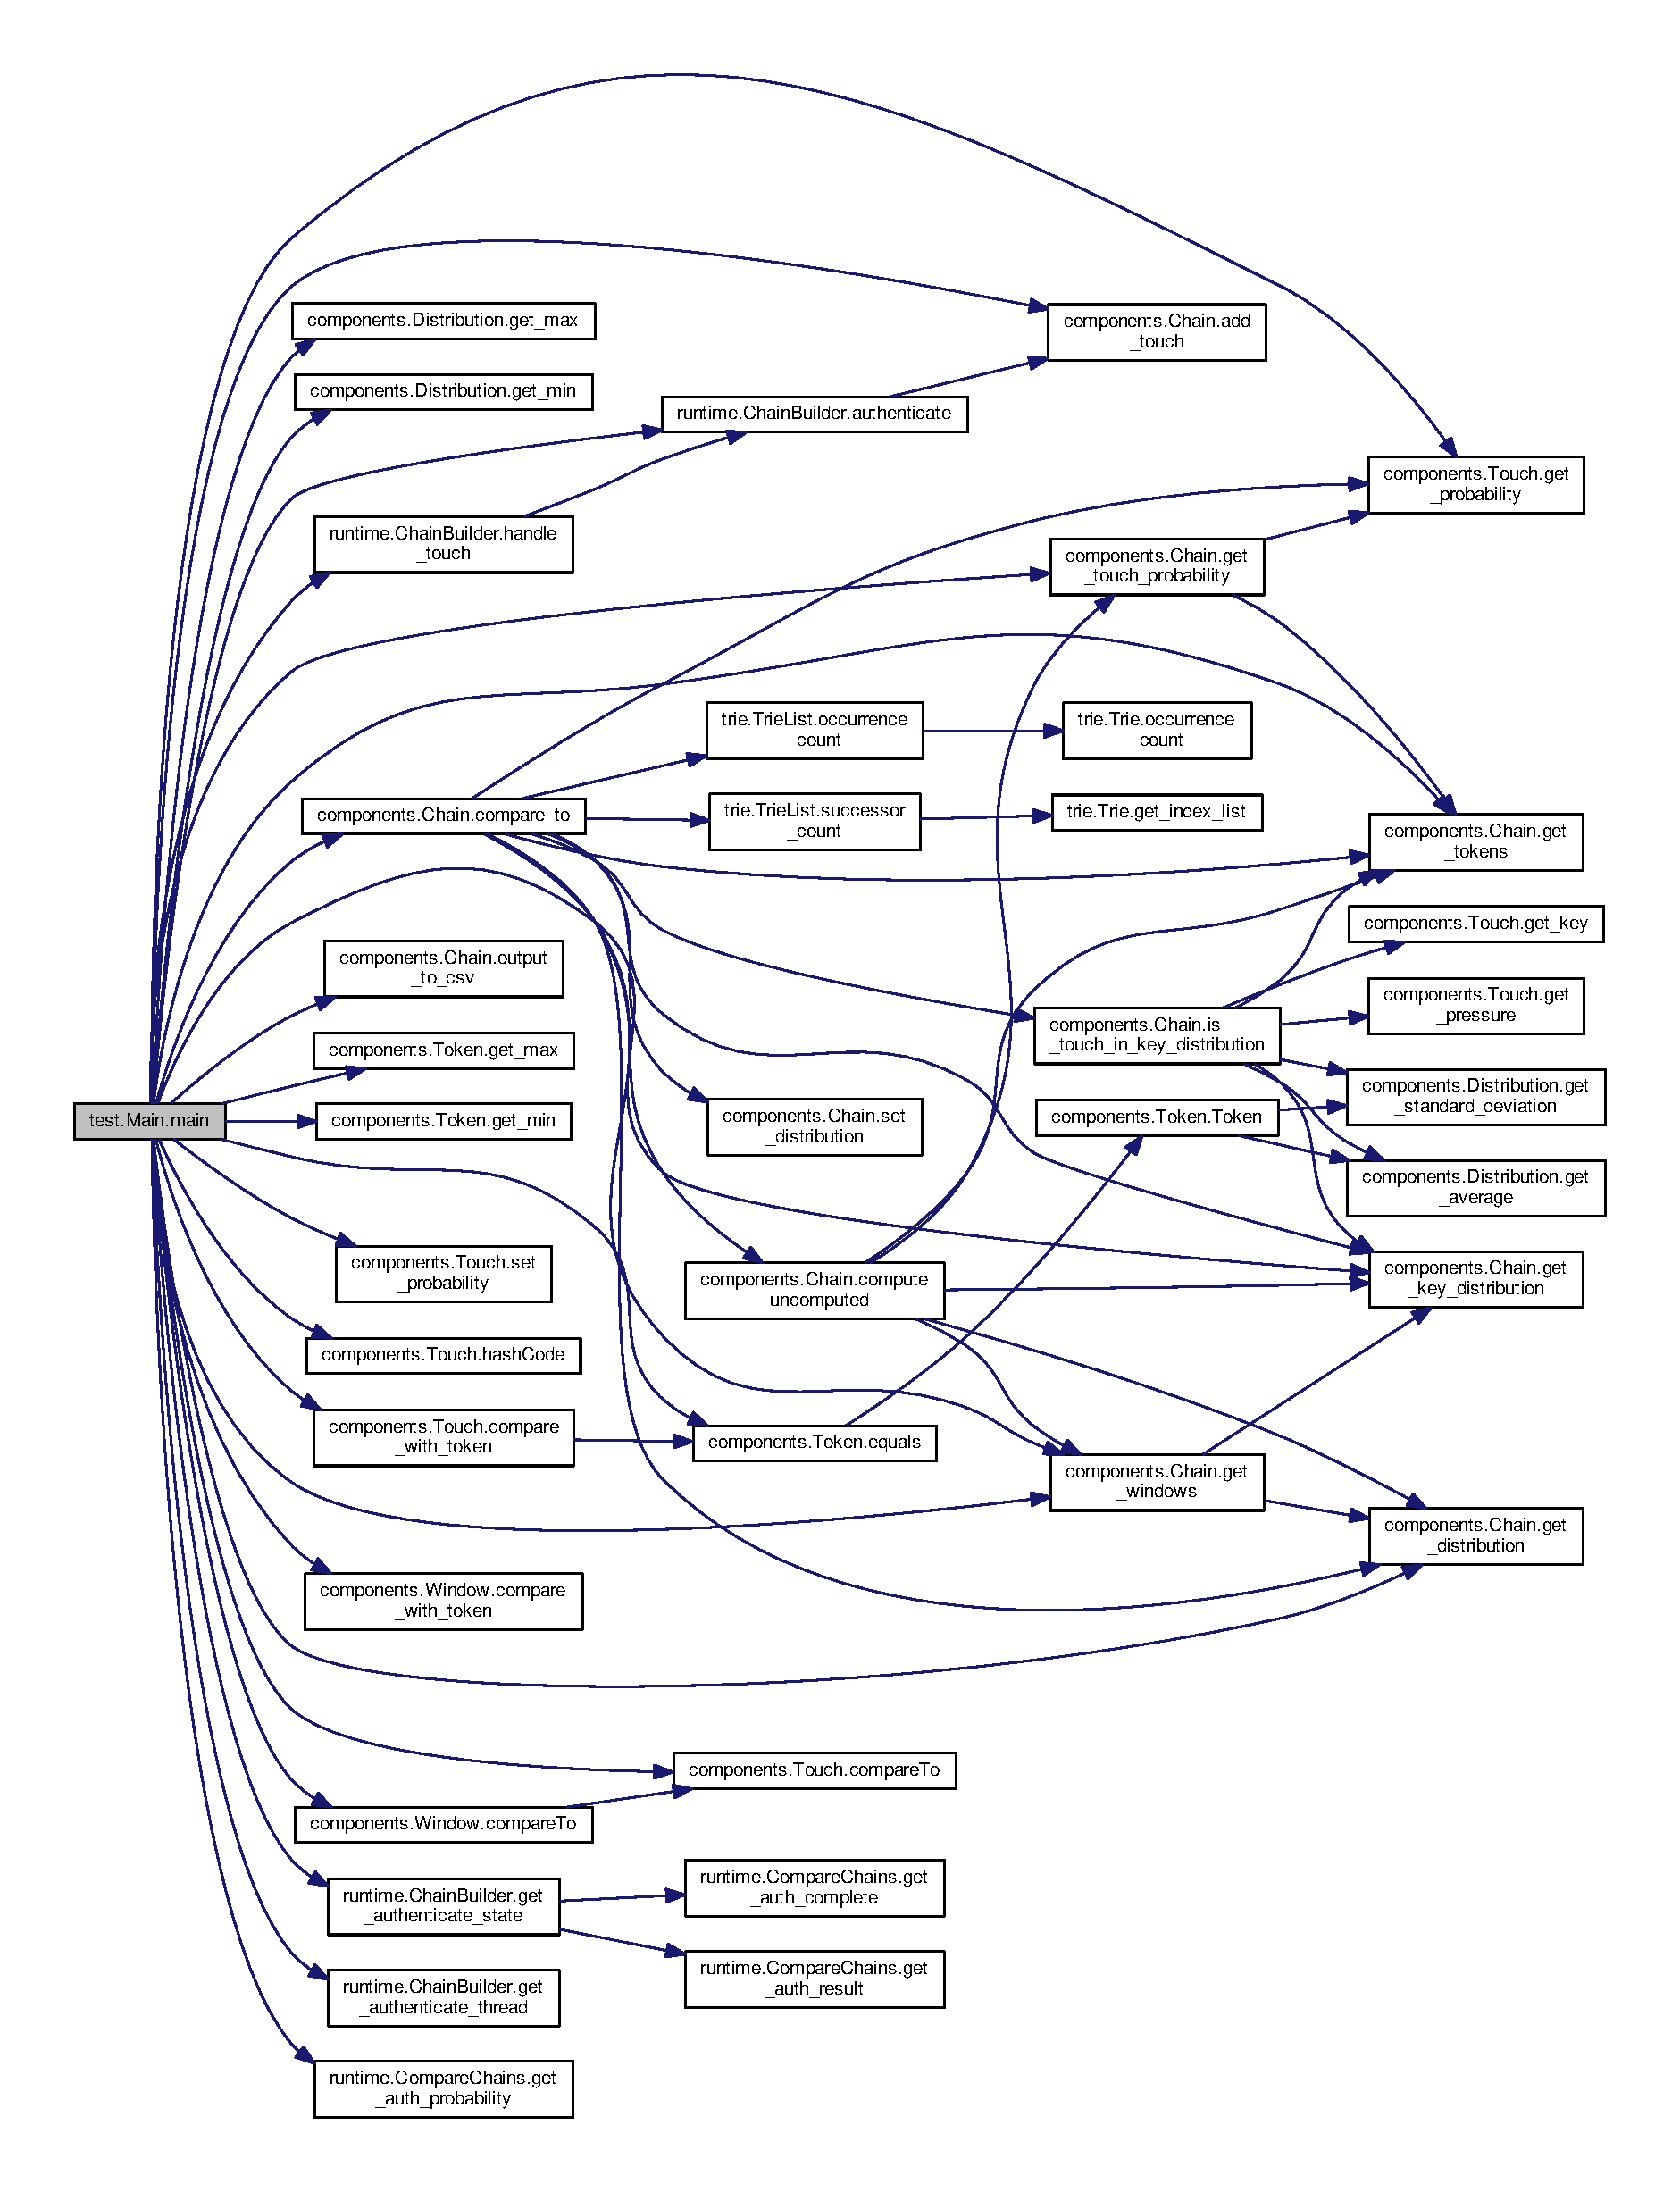
\includegraphics[width=350pt]{classtest_1_1_main_a7204edbad3d2a9d9784c3fa9786326cc_cgraph}
\end{center}
\end{figure}




Here is the caller graph for this function\+:\nopagebreak
\begin{figure}[H]
\begin{center}
\leavevmode
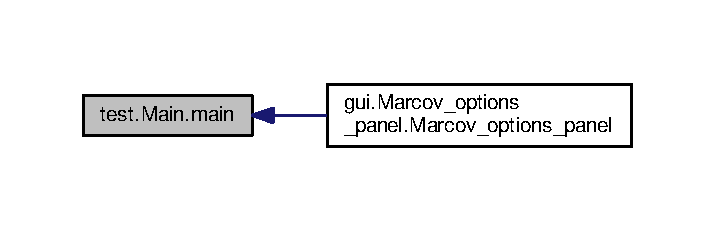
\includegraphics[width=343pt]{classtest_1_1_main_a7204edbad3d2a9d9784c3fa9786326cc_icgraph}
\end{center}
\end{figure}




The documentation for this class was generated from the following file\+:\begin{DoxyCompactItemize}
\item 
/home/element/\+P\+U\+F/\+Keyboard/java\+\_\+scripts/java\+\_\+marcov\+\_\+model/src/test/\hyperlink{_main_8java}{Main.\+java}\end{DoxyCompactItemize}

\hypertarget{classgui_1_1_marcov__console__panel}{}\section{gui.\+Marcov\+\_\+console\+\_\+panel Class Reference}
\label{classgui_1_1_marcov__console__panel}\index{gui.\+Marcov\+\_\+console\+\_\+panel@{gui.\+Marcov\+\_\+console\+\_\+panel}}
Inheritance diagram for gui.\+Marcov\+\_\+console\+\_\+panel\+:\begin{figure}[H]
\begin{center}
\leavevmode
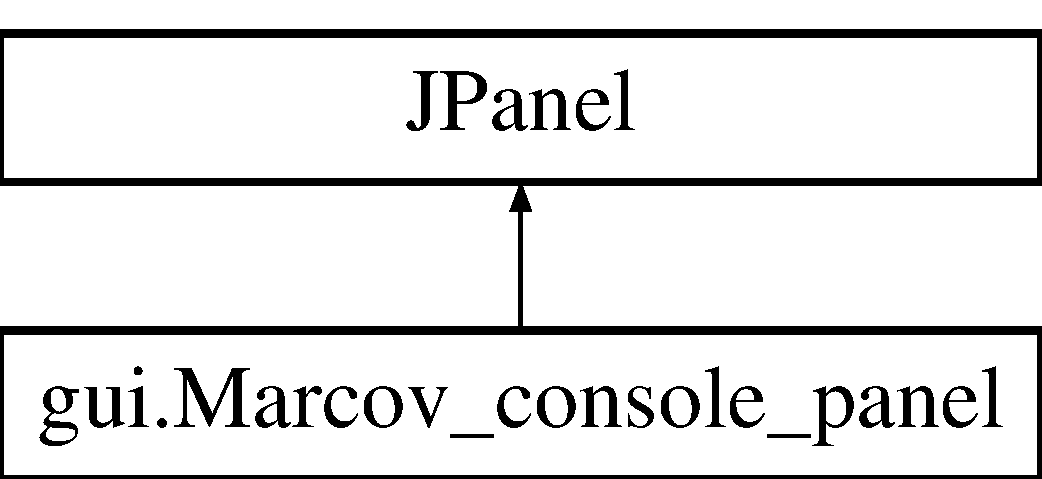
\includegraphics[height=2.000000cm]{classgui_1_1_marcov__console__panel}
\end{center}
\end{figure}
\subsection*{Public Member Functions}
\begin{DoxyCompactItemize}
\item 
\hyperlink{classgui_1_1_marcov__console__panel_a7d160acfa85d8f3c3d49dcdde384e288}{Marcov\+\_\+console\+\_\+panel} ()
\end{DoxyCompactItemize}


\subsection{Constructor \& Destructor Documentation}
\index{gui\+::\+Marcov\+\_\+console\+\_\+panel@{gui\+::\+Marcov\+\_\+console\+\_\+panel}!Marcov\+\_\+console\+\_\+panel@{Marcov\+\_\+console\+\_\+panel}}
\index{Marcov\+\_\+console\+\_\+panel@{Marcov\+\_\+console\+\_\+panel}!gui\+::\+Marcov\+\_\+console\+\_\+panel@{gui\+::\+Marcov\+\_\+console\+\_\+panel}}
\subsubsection[{\texorpdfstring{Marcov\+\_\+console\+\_\+panel()}{Marcov_console_panel()}}]{\setlength{\rightskip}{0pt plus 5cm}gui.\+Marcov\+\_\+console\+\_\+panel.\+Marcov\+\_\+console\+\_\+panel (
\begin{DoxyParamCaption}
{}
\end{DoxyParamCaption}
)}\hypertarget{classgui_1_1_marcov__console__panel_a7d160acfa85d8f3c3d49dcdde384e288}{}\label{classgui_1_1_marcov__console__panel_a7d160acfa85d8f3c3d49dcdde384e288}


The documentation for this class was generated from the following file\+:\begin{DoxyCompactItemize}
\item 
/home/element/\+P\+U\+F/\+Keyboard/java\+\_\+scripts/java\+\_\+marcov\+\_\+model/src/gui/\hyperlink{_marcov__console__panel_8java}{Marcov\+\_\+console\+\_\+panel.\+java}\end{DoxyCompactItemize}

\hypertarget{classgui_1_1_marcov__file__display__panel}{}\section{gui.\+Marcov\+\_\+file\+\_\+display\+\_\+panel Class Reference}
\label{classgui_1_1_marcov__file__display__panel}\index{gui.\+Marcov\+\_\+file\+\_\+display\+\_\+panel@{gui.\+Marcov\+\_\+file\+\_\+display\+\_\+panel}}
Inheritance diagram for gui.\+Marcov\+\_\+file\+\_\+display\+\_\+panel\+:\begin{figure}[H]
\begin{center}
\leavevmode
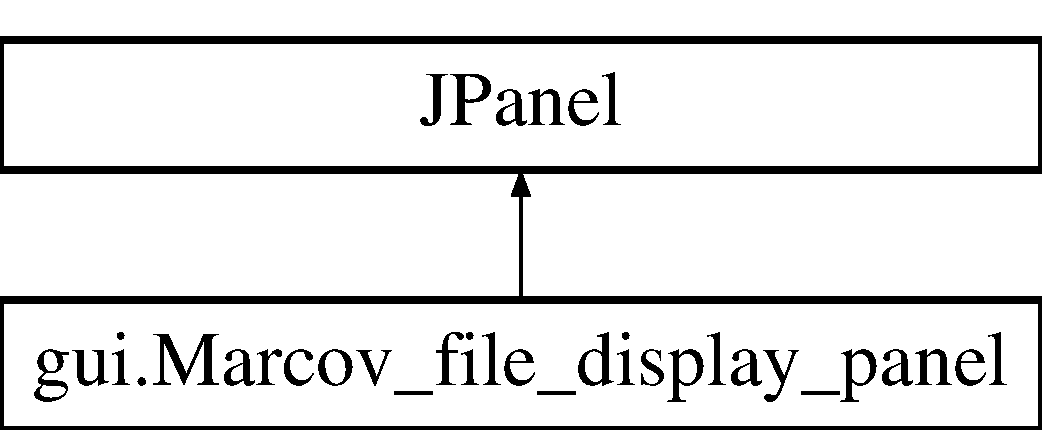
\includegraphics[height=2.000000cm]{classgui_1_1_marcov__file__display__panel}
\end{center}
\end{figure}
\subsection*{Public Member Functions}
\begin{DoxyCompactItemize}
\item 
\hyperlink{classgui_1_1_marcov__file__display__panel_a037887da35a96cb1571c80794a91bc2e}{Marcov\+\_\+file\+\_\+display\+\_\+panel} ()
\end{DoxyCompactItemize}


\subsection{Constructor \& Destructor Documentation}
\index{gui\+::\+Marcov\+\_\+file\+\_\+display\+\_\+panel@{gui\+::\+Marcov\+\_\+file\+\_\+display\+\_\+panel}!Marcov\+\_\+file\+\_\+display\+\_\+panel@{Marcov\+\_\+file\+\_\+display\+\_\+panel}}
\index{Marcov\+\_\+file\+\_\+display\+\_\+panel@{Marcov\+\_\+file\+\_\+display\+\_\+panel}!gui\+::\+Marcov\+\_\+file\+\_\+display\+\_\+panel@{gui\+::\+Marcov\+\_\+file\+\_\+display\+\_\+panel}}
\subsubsection[{\texorpdfstring{Marcov\+\_\+file\+\_\+display\+\_\+panel()}{Marcov_file_display_panel()}}]{\setlength{\rightskip}{0pt plus 5cm}gui.\+Marcov\+\_\+file\+\_\+display\+\_\+panel.\+Marcov\+\_\+file\+\_\+display\+\_\+panel (
\begin{DoxyParamCaption}
{}
\end{DoxyParamCaption}
)}\hypertarget{classgui_1_1_marcov__file__display__panel_a037887da35a96cb1571c80794a91bc2e}{}\label{classgui_1_1_marcov__file__display__panel_a037887da35a96cb1571c80794a91bc2e}


The documentation for this class was generated from the following file\+:\begin{DoxyCompactItemize}
\item 
/home/element/\+P\+U\+F/\+Keyboard/java\+\_\+scripts/java\+\_\+marcov\+\_\+model/src/gui/\hyperlink{_marcov__file__display__panel_8java}{Marcov\+\_\+file\+\_\+display\+\_\+panel.\+java}\end{DoxyCompactItemize}

\hypertarget{classgui_1_1_marcov__frame}{}\section{gui.\+Marcov\+\_\+frame Class Reference}
\label{classgui_1_1_marcov__frame}\index{gui.\+Marcov\+\_\+frame@{gui.\+Marcov\+\_\+frame}}


Display frame to contain buttons for running test code and panels to view results.  




Inheritance diagram for gui.\+Marcov\+\_\+frame\+:\nopagebreak
\begin{figure}[H]
\begin{center}
\leavevmode
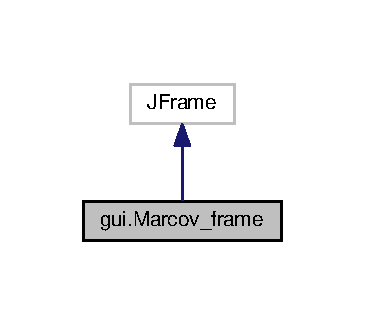
\includegraphics[width=175pt]{classgui_1_1_marcov__frame__inherit__graph}
\end{center}
\end{figure}


Collaboration diagram for gui.\+Marcov\+\_\+frame\+:\nopagebreak
\begin{figure}[H]
\begin{center}
\leavevmode
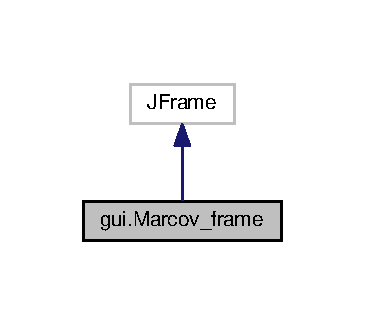
\includegraphics[width=175pt]{classgui_1_1_marcov__frame__coll__graph}
\end{center}
\end{figure}
\subsection*{Public Member Functions}
\begin{DoxyCompactItemize}
\item 
\hyperlink{classgui_1_1_marcov__frame_aeecc6459e2ff204f7212bf60f6c9d609}{Marcov\+\_\+frame} ()
\item 
void \hyperlink{classgui_1_1_marcov__frame_ac4a093f65a00cef89c56f3e63d23d429}{close} ()
\end{DoxyCompactItemize}


\subsection{Detailed Description}
Display frame to contain buttons for running test code and panels to view results. 



\subsection{Constructor \& Destructor Documentation}
\index{gui\+::\+Marcov\+\_\+frame@{gui\+::\+Marcov\+\_\+frame}!Marcov\+\_\+frame@{Marcov\+\_\+frame}}
\index{Marcov\+\_\+frame@{Marcov\+\_\+frame}!gui\+::\+Marcov\+\_\+frame@{gui\+::\+Marcov\+\_\+frame}}
\subsubsection[{\texorpdfstring{Marcov\+\_\+frame()}{Marcov_frame()}}]{\setlength{\rightskip}{0pt plus 5cm}gui.\+Marcov\+\_\+frame.\+Marcov\+\_\+frame (
\begin{DoxyParamCaption}
{}
\end{DoxyParamCaption}
)}\hypertarget{classgui_1_1_marcov__frame_aeecc6459e2ff204f7212bf60f6c9d609}{}\label{classgui_1_1_marcov__frame_aeecc6459e2ff204f7212bf60f6c9d609}


\subsection{Member Function Documentation}
\index{gui\+::\+Marcov\+\_\+frame@{gui\+::\+Marcov\+\_\+frame}!close@{close}}
\index{close@{close}!gui\+::\+Marcov\+\_\+frame@{gui\+::\+Marcov\+\_\+frame}}
\subsubsection[{\texorpdfstring{close()}{close()}}]{\setlength{\rightskip}{0pt plus 5cm}void gui.\+Marcov\+\_\+frame.\+close (
\begin{DoxyParamCaption}
{}
\end{DoxyParamCaption}
)}\hypertarget{classgui_1_1_marcov__frame_ac4a093f65a00cef89c56f3e63d23d429}{}\label{classgui_1_1_marcov__frame_ac4a093f65a00cef89c56f3e63d23d429}


The documentation for this class was generated from the following file\+:\begin{DoxyCompactItemize}
\item 
/home/element/\+P\+U\+F/\+Keyboard/java\+\_\+scripts/java\+\_\+marcov\+\_\+model/src/gui/\hyperlink{_marcov__frame_8java}{Marcov\+\_\+frame.\+java}\end{DoxyCompactItemize}

\hypertarget{classgui_1_1_marcov__options__panel}{}\section{gui.\+Marcov\+\_\+options\+\_\+panel Class Reference}
\label{classgui_1_1_marcov__options__panel}\index{gui.\+Marcov\+\_\+options\+\_\+panel@{gui.\+Marcov\+\_\+options\+\_\+panel}}


Inheritance diagram for gui.\+Marcov\+\_\+options\+\_\+panel\+:\nopagebreak
\begin{figure}[H]
\begin{center}
\leavevmode
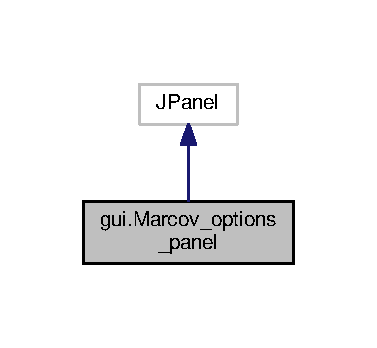
\includegraphics[width=181pt]{classgui_1_1_marcov__options__panel__inherit__graph}
\end{center}
\end{figure}


Collaboration diagram for gui.\+Marcov\+\_\+options\+\_\+panel\+:\nopagebreak
\begin{figure}[H]
\begin{center}
\leavevmode
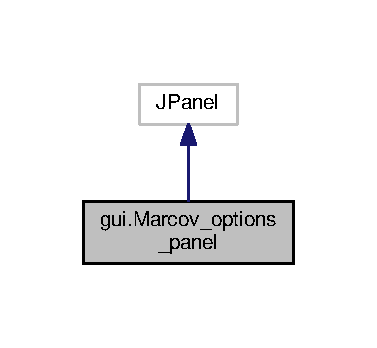
\includegraphics[width=181pt]{classgui_1_1_marcov__options__panel__coll__graph}
\end{center}
\end{figure}
\subsection*{Public Member Functions}
\begin{DoxyCompactItemize}
\item 
\hyperlink{classgui_1_1_marcov__options__panel_a00bf246da4a188f42d43c60a243f26ad}{Marcov\+\_\+options\+\_\+panel} ()
\end{DoxyCompactItemize}


\subsection{Constructor \& Destructor Documentation}
\index{gui\+::\+Marcov\+\_\+options\+\_\+panel@{gui\+::\+Marcov\+\_\+options\+\_\+panel}!Marcov\+\_\+options\+\_\+panel@{Marcov\+\_\+options\+\_\+panel}}
\index{Marcov\+\_\+options\+\_\+panel@{Marcov\+\_\+options\+\_\+panel}!gui\+::\+Marcov\+\_\+options\+\_\+panel@{gui\+::\+Marcov\+\_\+options\+\_\+panel}}
\subsubsection[{\texorpdfstring{Marcov\+\_\+options\+\_\+panel()}{Marcov_options_panel()}}]{\setlength{\rightskip}{0pt plus 5cm}gui.\+Marcov\+\_\+options\+\_\+panel.\+Marcov\+\_\+options\+\_\+panel (
\begin{DoxyParamCaption}
{}
\end{DoxyParamCaption}
)}\hypertarget{classgui_1_1_marcov__options__panel_a00bf246da4a188f42d43c60a243f26ad}{}\label{classgui_1_1_marcov__options__panel_a00bf246da4a188f42d43c60a243f26ad}


Here is the call graph for this function\+:\nopagebreak
\begin{figure}[H]
\begin{center}
\leavevmode
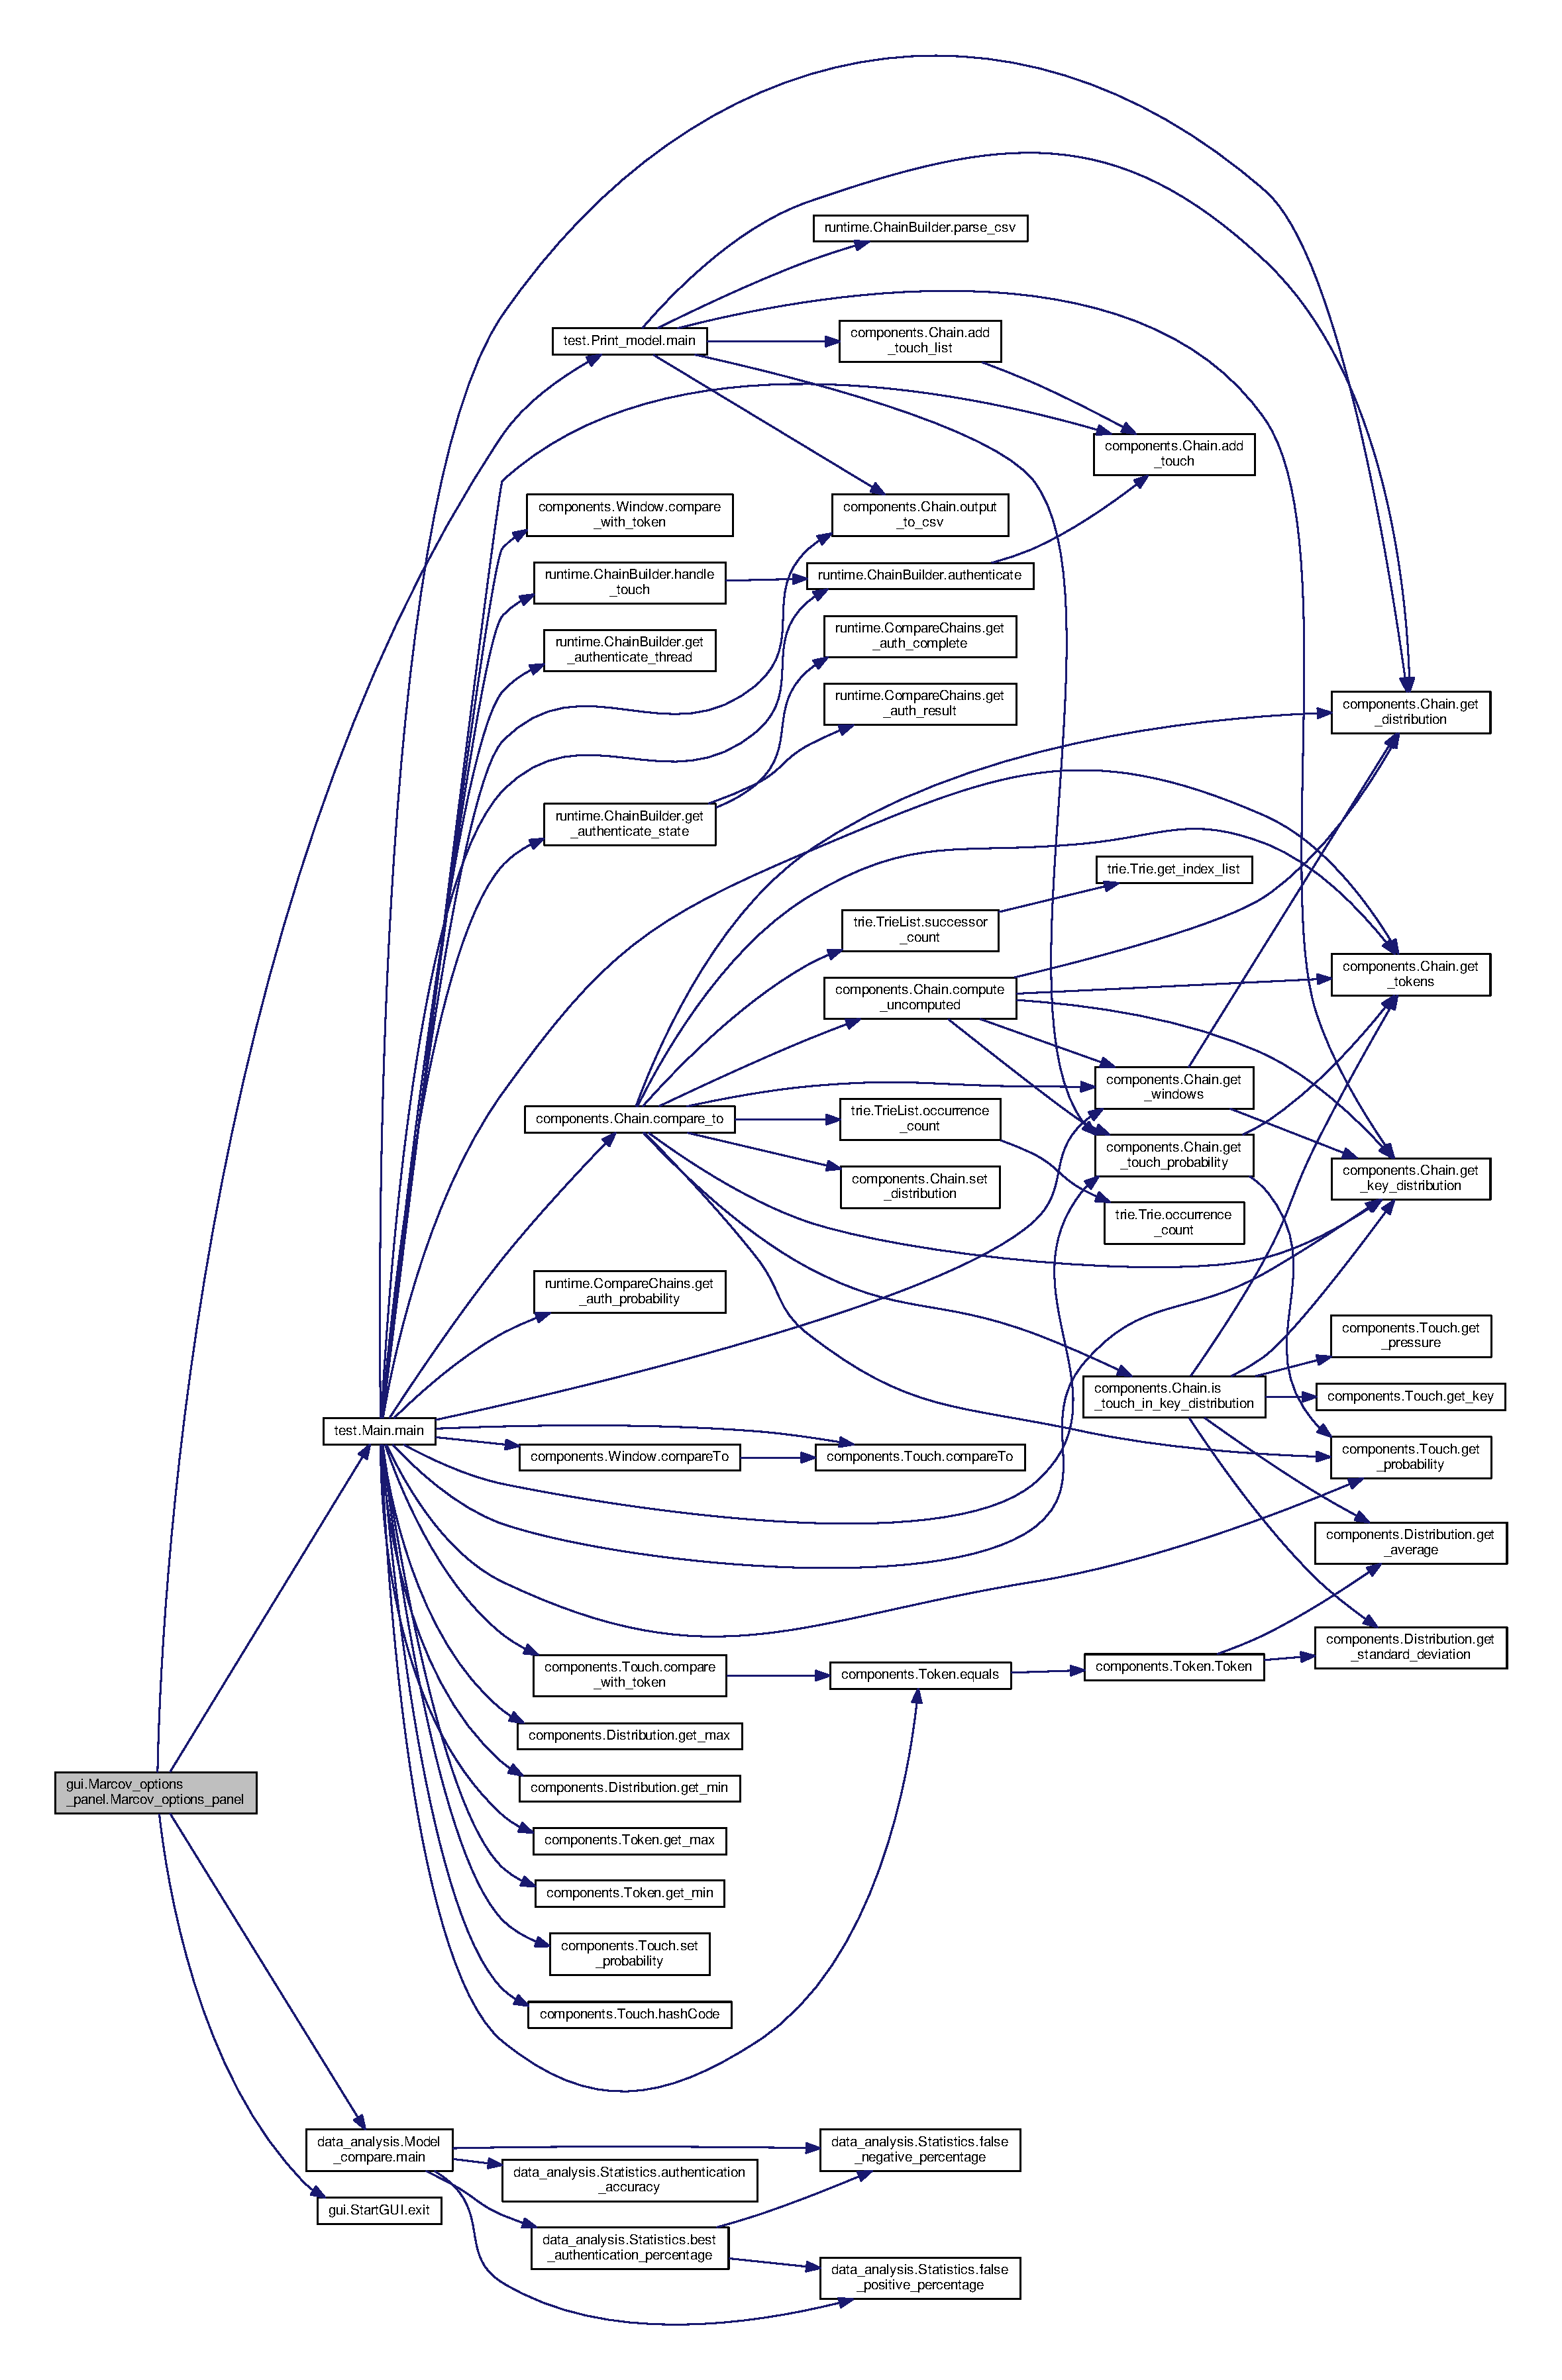
\includegraphics[width=350pt]{classgui_1_1_marcov__options__panel_a00bf246da4a188f42d43c60a243f26ad_cgraph}
\end{center}
\end{figure}




The documentation for this class was generated from the following file\+:\begin{DoxyCompactItemize}
\item 
/home/element/\+P\+U\+F/\+Keyboard/java\+\_\+scripts/java\+\_\+marcov\+\_\+model/src/gui/\hyperlink{_marcov__options__panel_8java}{Marcov\+\_\+options\+\_\+panel.\+java}\end{DoxyCompactItemize}

\hypertarget{classdata__analysis_1_1_model__compare}{}\section{data\+\_\+analysis.\+Model\+\_\+compare Class Reference}
\label{classdata__analysis_1_1_model__compare}\index{data\+\_\+analysis.\+Model\+\_\+compare@{data\+\_\+analysis.\+Model\+\_\+compare}}
\subsection*{Static Public Member Functions}
\begin{DoxyCompactItemize}
\item 
static void \hyperlink{classdata__analysis_1_1_model__compare_a439121c41a799d062e452218d88a59a9}{main} (String\mbox{[}$\,$\mbox{]} args)
\end{DoxyCompactItemize}


\subsection{Detailed Description}
The purpose of this class is to test out the model compare process on data that has been collected The data to used will be contained in the data\+\_\+sets folder input\+: data\+\_\+sets folder output\+: model\+\_\+compare\+\_\+output.\+txt 

\subsection{Member Function Documentation}
\index{data\+\_\+analysis\+::\+Model\+\_\+compare@{data\+\_\+analysis\+::\+Model\+\_\+compare}!main@{main}}
\index{main@{main}!data\+\_\+analysis\+::\+Model\+\_\+compare@{data\+\_\+analysis\+::\+Model\+\_\+compare}}
\subsubsection[{\texorpdfstring{main(\+String[] args)}{main(String[] args)}}]{\setlength{\rightskip}{0pt plus 5cm}static void data\+\_\+analysis.\+Model\+\_\+compare.\+main (
\begin{DoxyParamCaption}
\item[{String\mbox{[}$\,$\mbox{]}}]{args}
\end{DoxyParamCaption}
)\hspace{0.3cm}{\ttfamily [static]}}\hypertarget{classdata__analysis_1_1_model__compare_a439121c41a799d062e452218d88a59a9}{}\label{classdata__analysis_1_1_model__compare_a439121c41a799d062e452218d88a59a9}
create a number of tests with different parameters 

The documentation for this class was generated from the following file\+:\begin{DoxyCompactItemize}
\item 
/home/element/\+P\+U\+F/\+Keyboard/java\+\_\+scripts/java\+\_\+marcov\+\_\+model/src/data\+\_\+analysis/\hyperlink{_model__compare_8java}{Model\+\_\+compare.\+java}\end{DoxyCompactItemize}

\hypertarget{classdata__analysis_1_1_model__compare__thread}{}\section{data\+\_\+analysis.\+Model\+\_\+compare\+\_\+thread Class Reference}
\label{classdata__analysis_1_1_model__compare__thread}\index{data\+\_\+analysis.\+Model\+\_\+compare\+\_\+thread@{data\+\_\+analysis.\+Model\+\_\+compare\+\_\+thread}}
Inheritance diagram for data\+\_\+analysis.\+Model\+\_\+compare\+\_\+thread\+:\begin{figure}[H]
\begin{center}
\leavevmode
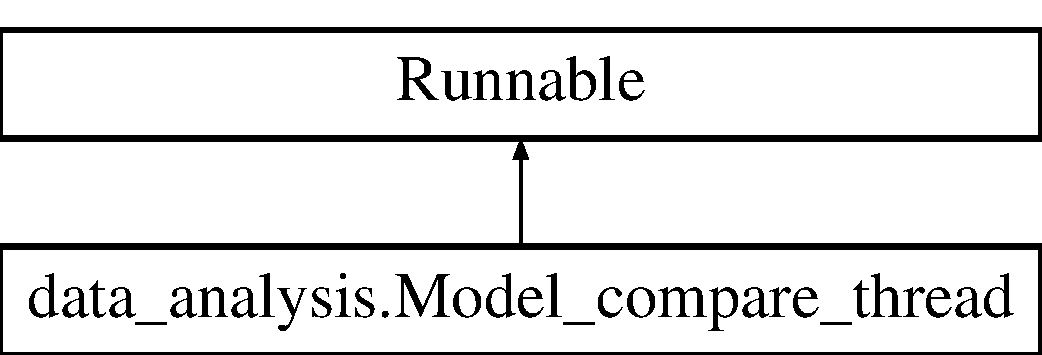
\includegraphics[height=2.000000cm]{classdata__analysis_1_1_model__compare__thread}
\end{center}
\end{figure}
\subsection*{Public Member Functions}
\begin{DoxyCompactItemize}
\item 
\hyperlink{classdata__analysis_1_1_model__compare__thread_a0ee9d1dece56959345e6c0e369b06e38}{Model\+\_\+compare\+\_\+thread} (String base\+\_\+data\+\_\+path, String auth\+\_\+data\+\_\+path, int base\+\_\+model\+\_\+size, int auth\+\_\+model\+\_\+size, int window\+\_\+size, int token\+\_\+size, int threshold)
\begin{DoxyCompactList}\small\item\em constructor, allowing user to set different probperties of the model compairason for testing \end{DoxyCompactList}\item 
void \hyperlink{classdata__analysis_1_1_model__compare__thread_ad75761fec2f2e5e2dd2679b6a120f2a4}{run} ()
\item 
String \hyperlink{classdata__analysis_1_1_model__compare__thread_af3bfecb6b0ad04d38fcfa2d4a0c69866}{get\+\_\+base\+\_\+data\+\_\+path} ()
\item 
String \hyperlink{classdata__analysis_1_1_model__compare__thread_a2b890e51f20cbea9ee865d5baae689a7}{get\+\_\+auth\+\_\+data\+\_\+path} ()
\item 
int \hyperlink{classdata__analysis_1_1_model__compare__thread_a268439415f6bd1f912cbcff8af77b636}{get\+\_\+window\+\_\+size} ()
\item 
int \hyperlink{classdata__analysis_1_1_model__compare__thread_a7d81e3cf81f4222d4da104d9429b578e}{get\+\_\+token\+\_\+size} ()
\item 
int \hyperlink{classdata__analysis_1_1_model__compare__thread_a59482784f581ddbaf509bf81cc0c249b}{get\+\_\+threshold} ()
\item 
int \hyperlink{classdata__analysis_1_1_model__compare__thread_a963240b77cca8d407e93fc733f0aed7c}{get\+\_\+base\+\_\+model\+\_\+size} ()
\item 
int \hyperlink{classdata__analysis_1_1_model__compare__thread_a22c1e624e263f61b4d9dee5fb60dd1b8}{get\+\_\+auth\+\_\+model\+\_\+size} ()
\item 
List$<$ Double $>$ \hyperlink{classdata__analysis_1_1_model__compare__thread_af0dbf695248868d7bb401be50f45b386}{get\+\_\+auth\+\_\+probability\+\_\+list} ()
\end{DoxyCompactItemize}
\subsection*{Public Attributes}
\begin{DoxyCompactItemize}
\item 
double \hyperlink{classdata__analysis_1_1_model__compare__thread_a6213d96c54d70f9e8a2d01010414ecd3}{max\+\_\+authentication\+\_\+probability}
\item 
double \hyperlink{classdata__analysis_1_1_model__compare__thread_a8a9c58abe260de662f846876d4f7fed2}{min\+\_\+authentication\+\_\+probability}
\item 
double \hyperlink{classdata__analysis_1_1_model__compare__thread_a9a8a983509cfefb0d73b813f45fd2ef1}{average\+\_\+authentication\+\_\+probability}
\end{DoxyCompactItemize}


\subsection{Detailed Description}
this thread allows the preforming of a test compairason. when the compairason is finished, an instance variable will be set indicating different results. 

\subsection{Constructor \& Destructor Documentation}
\index{data\+\_\+analysis\+::\+Model\+\_\+compare\+\_\+thread@{data\+\_\+analysis\+::\+Model\+\_\+compare\+\_\+thread}!Model\+\_\+compare\+\_\+thread@{Model\+\_\+compare\+\_\+thread}}
\index{Model\+\_\+compare\+\_\+thread@{Model\+\_\+compare\+\_\+thread}!data\+\_\+analysis\+::\+Model\+\_\+compare\+\_\+thread@{data\+\_\+analysis\+::\+Model\+\_\+compare\+\_\+thread}}
\subsubsection[{\texorpdfstring{Model\+\_\+compare\+\_\+thread(\+String base\+\_\+data\+\_\+path, String auth\+\_\+data\+\_\+path, int base\+\_\+model\+\_\+size, int auth\+\_\+model\+\_\+size, int window\+\_\+size, int token\+\_\+size, int threshold)}{Model_compare_thread(String base_data_path, String auth_data_path, int base_model_size, int auth_model_size, int window_size, int token_size, int threshold)}}]{\setlength{\rightskip}{0pt plus 5cm}data\+\_\+analysis.\+Model\+\_\+compare\+\_\+thread.\+Model\+\_\+compare\+\_\+thread (
\begin{DoxyParamCaption}
\item[{String}]{base\+\_\+data\+\_\+path, }
\item[{String}]{auth\+\_\+data\+\_\+path, }
\item[{int}]{base\+\_\+model\+\_\+size, }
\item[{int}]{auth\+\_\+model\+\_\+size, }
\item[{int}]{window\+\_\+size, }
\item[{int}]{token\+\_\+size, }
\item[{int}]{threshold}
\end{DoxyParamCaption}
)}\hypertarget{classdata__analysis_1_1_model__compare__thread_a0ee9d1dece56959345e6c0e369b06e38}{}\label{classdata__analysis_1_1_model__compare__thread_a0ee9d1dece56959345e6c0e369b06e38}


constructor, allowing user to set different probperties of the model compairason for testing 



\subsection{Member Function Documentation}
\index{data\+\_\+analysis\+::\+Model\+\_\+compare\+\_\+thread@{data\+\_\+analysis\+::\+Model\+\_\+compare\+\_\+thread}!get\+\_\+auth\+\_\+data\+\_\+path@{get\+\_\+auth\+\_\+data\+\_\+path}}
\index{get\+\_\+auth\+\_\+data\+\_\+path@{get\+\_\+auth\+\_\+data\+\_\+path}!data\+\_\+analysis\+::\+Model\+\_\+compare\+\_\+thread@{data\+\_\+analysis\+::\+Model\+\_\+compare\+\_\+thread}}
\subsubsection[{\texorpdfstring{get\+\_\+auth\+\_\+data\+\_\+path()}{get_auth_data_path()}}]{\setlength{\rightskip}{0pt plus 5cm}String data\+\_\+analysis.\+Model\+\_\+compare\+\_\+thread.\+get\+\_\+auth\+\_\+data\+\_\+path (
\begin{DoxyParamCaption}
{}
\end{DoxyParamCaption}
)}\hypertarget{classdata__analysis_1_1_model__compare__thread_a2b890e51f20cbea9ee865d5baae689a7}{}\label{classdata__analysis_1_1_model__compare__thread_a2b890e51f20cbea9ee865d5baae689a7}
\index{data\+\_\+analysis\+::\+Model\+\_\+compare\+\_\+thread@{data\+\_\+analysis\+::\+Model\+\_\+compare\+\_\+thread}!get\+\_\+auth\+\_\+model\+\_\+size@{get\+\_\+auth\+\_\+model\+\_\+size}}
\index{get\+\_\+auth\+\_\+model\+\_\+size@{get\+\_\+auth\+\_\+model\+\_\+size}!data\+\_\+analysis\+::\+Model\+\_\+compare\+\_\+thread@{data\+\_\+analysis\+::\+Model\+\_\+compare\+\_\+thread}}
\subsubsection[{\texorpdfstring{get\+\_\+auth\+\_\+model\+\_\+size()}{get_auth_model_size()}}]{\setlength{\rightskip}{0pt plus 5cm}int data\+\_\+analysis.\+Model\+\_\+compare\+\_\+thread.\+get\+\_\+auth\+\_\+model\+\_\+size (
\begin{DoxyParamCaption}
{}
\end{DoxyParamCaption}
)}\hypertarget{classdata__analysis_1_1_model__compare__thread_a22c1e624e263f61b4d9dee5fb60dd1b8}{}\label{classdata__analysis_1_1_model__compare__thread_a22c1e624e263f61b4d9dee5fb60dd1b8}
\index{data\+\_\+analysis\+::\+Model\+\_\+compare\+\_\+thread@{data\+\_\+analysis\+::\+Model\+\_\+compare\+\_\+thread}!get\+\_\+auth\+\_\+probability\+\_\+list@{get\+\_\+auth\+\_\+probability\+\_\+list}}
\index{get\+\_\+auth\+\_\+probability\+\_\+list@{get\+\_\+auth\+\_\+probability\+\_\+list}!data\+\_\+analysis\+::\+Model\+\_\+compare\+\_\+thread@{data\+\_\+analysis\+::\+Model\+\_\+compare\+\_\+thread}}
\subsubsection[{\texorpdfstring{get\+\_\+auth\+\_\+probability\+\_\+list()}{get_auth_probability_list()}}]{\setlength{\rightskip}{0pt plus 5cm}List$<$Double$>$ data\+\_\+analysis.\+Model\+\_\+compare\+\_\+thread.\+get\+\_\+auth\+\_\+probability\+\_\+list (
\begin{DoxyParamCaption}
{}
\end{DoxyParamCaption}
)}\hypertarget{classdata__analysis_1_1_model__compare__thread_af0dbf695248868d7bb401be50f45b386}{}\label{classdata__analysis_1_1_model__compare__thread_af0dbf695248868d7bb401be50f45b386}
\index{data\+\_\+analysis\+::\+Model\+\_\+compare\+\_\+thread@{data\+\_\+analysis\+::\+Model\+\_\+compare\+\_\+thread}!get\+\_\+base\+\_\+data\+\_\+path@{get\+\_\+base\+\_\+data\+\_\+path}}
\index{get\+\_\+base\+\_\+data\+\_\+path@{get\+\_\+base\+\_\+data\+\_\+path}!data\+\_\+analysis\+::\+Model\+\_\+compare\+\_\+thread@{data\+\_\+analysis\+::\+Model\+\_\+compare\+\_\+thread}}
\subsubsection[{\texorpdfstring{get\+\_\+base\+\_\+data\+\_\+path()}{get_base_data_path()}}]{\setlength{\rightskip}{0pt plus 5cm}String data\+\_\+analysis.\+Model\+\_\+compare\+\_\+thread.\+get\+\_\+base\+\_\+data\+\_\+path (
\begin{DoxyParamCaption}
{}
\end{DoxyParamCaption}
)}\hypertarget{classdata__analysis_1_1_model__compare__thread_af3bfecb6b0ad04d38fcfa2d4a0c69866}{}\label{classdata__analysis_1_1_model__compare__thread_af3bfecb6b0ad04d38fcfa2d4a0c69866}
\index{data\+\_\+analysis\+::\+Model\+\_\+compare\+\_\+thread@{data\+\_\+analysis\+::\+Model\+\_\+compare\+\_\+thread}!get\+\_\+base\+\_\+model\+\_\+size@{get\+\_\+base\+\_\+model\+\_\+size}}
\index{get\+\_\+base\+\_\+model\+\_\+size@{get\+\_\+base\+\_\+model\+\_\+size}!data\+\_\+analysis\+::\+Model\+\_\+compare\+\_\+thread@{data\+\_\+analysis\+::\+Model\+\_\+compare\+\_\+thread}}
\subsubsection[{\texorpdfstring{get\+\_\+base\+\_\+model\+\_\+size()}{get_base_model_size()}}]{\setlength{\rightskip}{0pt plus 5cm}int data\+\_\+analysis.\+Model\+\_\+compare\+\_\+thread.\+get\+\_\+base\+\_\+model\+\_\+size (
\begin{DoxyParamCaption}
{}
\end{DoxyParamCaption}
)}\hypertarget{classdata__analysis_1_1_model__compare__thread_a963240b77cca8d407e93fc733f0aed7c}{}\label{classdata__analysis_1_1_model__compare__thread_a963240b77cca8d407e93fc733f0aed7c}
\index{data\+\_\+analysis\+::\+Model\+\_\+compare\+\_\+thread@{data\+\_\+analysis\+::\+Model\+\_\+compare\+\_\+thread}!get\+\_\+threshold@{get\+\_\+threshold}}
\index{get\+\_\+threshold@{get\+\_\+threshold}!data\+\_\+analysis\+::\+Model\+\_\+compare\+\_\+thread@{data\+\_\+analysis\+::\+Model\+\_\+compare\+\_\+thread}}
\subsubsection[{\texorpdfstring{get\+\_\+threshold()}{get_threshold()}}]{\setlength{\rightskip}{0pt plus 5cm}int data\+\_\+analysis.\+Model\+\_\+compare\+\_\+thread.\+get\+\_\+threshold (
\begin{DoxyParamCaption}
{}
\end{DoxyParamCaption}
)}\hypertarget{classdata__analysis_1_1_model__compare__thread_a59482784f581ddbaf509bf81cc0c249b}{}\label{classdata__analysis_1_1_model__compare__thread_a59482784f581ddbaf509bf81cc0c249b}
\index{data\+\_\+analysis\+::\+Model\+\_\+compare\+\_\+thread@{data\+\_\+analysis\+::\+Model\+\_\+compare\+\_\+thread}!get\+\_\+token\+\_\+size@{get\+\_\+token\+\_\+size}}
\index{get\+\_\+token\+\_\+size@{get\+\_\+token\+\_\+size}!data\+\_\+analysis\+::\+Model\+\_\+compare\+\_\+thread@{data\+\_\+analysis\+::\+Model\+\_\+compare\+\_\+thread}}
\subsubsection[{\texorpdfstring{get\+\_\+token\+\_\+size()}{get_token_size()}}]{\setlength{\rightskip}{0pt plus 5cm}int data\+\_\+analysis.\+Model\+\_\+compare\+\_\+thread.\+get\+\_\+token\+\_\+size (
\begin{DoxyParamCaption}
{}
\end{DoxyParamCaption}
)}\hypertarget{classdata__analysis_1_1_model__compare__thread_a7d81e3cf81f4222d4da104d9429b578e}{}\label{classdata__analysis_1_1_model__compare__thread_a7d81e3cf81f4222d4da104d9429b578e}
\index{data\+\_\+analysis\+::\+Model\+\_\+compare\+\_\+thread@{data\+\_\+analysis\+::\+Model\+\_\+compare\+\_\+thread}!get\+\_\+window\+\_\+size@{get\+\_\+window\+\_\+size}}
\index{get\+\_\+window\+\_\+size@{get\+\_\+window\+\_\+size}!data\+\_\+analysis\+::\+Model\+\_\+compare\+\_\+thread@{data\+\_\+analysis\+::\+Model\+\_\+compare\+\_\+thread}}
\subsubsection[{\texorpdfstring{get\+\_\+window\+\_\+size()}{get_window_size()}}]{\setlength{\rightskip}{0pt plus 5cm}int data\+\_\+analysis.\+Model\+\_\+compare\+\_\+thread.\+get\+\_\+window\+\_\+size (
\begin{DoxyParamCaption}
{}
\end{DoxyParamCaption}
)}\hypertarget{classdata__analysis_1_1_model__compare__thread_a268439415f6bd1f912cbcff8af77b636}{}\label{classdata__analysis_1_1_model__compare__thread_a268439415f6bd1f912cbcff8af77b636}
\index{data\+\_\+analysis\+::\+Model\+\_\+compare\+\_\+thread@{data\+\_\+analysis\+::\+Model\+\_\+compare\+\_\+thread}!run@{run}}
\index{run@{run}!data\+\_\+analysis\+::\+Model\+\_\+compare\+\_\+thread@{data\+\_\+analysis\+::\+Model\+\_\+compare\+\_\+thread}}
\subsubsection[{\texorpdfstring{run()}{run()}}]{\setlength{\rightskip}{0pt plus 5cm}void data\+\_\+analysis.\+Model\+\_\+compare\+\_\+thread.\+run (
\begin{DoxyParamCaption}
{}
\end{DoxyParamCaption}
)}\hypertarget{classdata__analysis_1_1_model__compare__thread_ad75761fec2f2e5e2dd2679b6a120f2a4}{}\label{classdata__analysis_1_1_model__compare__thread_ad75761fec2f2e5e2dd2679b6a120f2a4}


\subsection{Member Data Documentation}
\index{data\+\_\+analysis\+::\+Model\+\_\+compare\+\_\+thread@{data\+\_\+analysis\+::\+Model\+\_\+compare\+\_\+thread}!average\+\_\+authentication\+\_\+probability@{average\+\_\+authentication\+\_\+probability}}
\index{average\+\_\+authentication\+\_\+probability@{average\+\_\+authentication\+\_\+probability}!data\+\_\+analysis\+::\+Model\+\_\+compare\+\_\+thread@{data\+\_\+analysis\+::\+Model\+\_\+compare\+\_\+thread}}
\subsubsection[{\texorpdfstring{average\+\_\+authentication\+\_\+probability}{average_authentication_probability}}]{\setlength{\rightskip}{0pt plus 5cm}double data\+\_\+analysis.\+Model\+\_\+compare\+\_\+thread.\+average\+\_\+authentication\+\_\+probability}\hypertarget{classdata__analysis_1_1_model__compare__thread_a9a8a983509cfefb0d73b813f45fd2ef1}{}\label{classdata__analysis_1_1_model__compare__thread_a9a8a983509cfefb0d73b813f45fd2ef1}
\index{data\+\_\+analysis\+::\+Model\+\_\+compare\+\_\+thread@{data\+\_\+analysis\+::\+Model\+\_\+compare\+\_\+thread}!max\+\_\+authentication\+\_\+probability@{max\+\_\+authentication\+\_\+probability}}
\index{max\+\_\+authentication\+\_\+probability@{max\+\_\+authentication\+\_\+probability}!data\+\_\+analysis\+::\+Model\+\_\+compare\+\_\+thread@{data\+\_\+analysis\+::\+Model\+\_\+compare\+\_\+thread}}
\subsubsection[{\texorpdfstring{max\+\_\+authentication\+\_\+probability}{max_authentication_probability}}]{\setlength{\rightskip}{0pt plus 5cm}double data\+\_\+analysis.\+Model\+\_\+compare\+\_\+thread.\+max\+\_\+authentication\+\_\+probability}\hypertarget{classdata__analysis_1_1_model__compare__thread_a6213d96c54d70f9e8a2d01010414ecd3}{}\label{classdata__analysis_1_1_model__compare__thread_a6213d96c54d70f9e8a2d01010414ecd3}
\index{data\+\_\+analysis\+::\+Model\+\_\+compare\+\_\+thread@{data\+\_\+analysis\+::\+Model\+\_\+compare\+\_\+thread}!min\+\_\+authentication\+\_\+probability@{min\+\_\+authentication\+\_\+probability}}
\index{min\+\_\+authentication\+\_\+probability@{min\+\_\+authentication\+\_\+probability}!data\+\_\+analysis\+::\+Model\+\_\+compare\+\_\+thread@{data\+\_\+analysis\+::\+Model\+\_\+compare\+\_\+thread}}
\subsubsection[{\texorpdfstring{min\+\_\+authentication\+\_\+probability}{min_authentication_probability}}]{\setlength{\rightskip}{0pt plus 5cm}double data\+\_\+analysis.\+Model\+\_\+compare\+\_\+thread.\+min\+\_\+authentication\+\_\+probability}\hypertarget{classdata__analysis_1_1_model__compare__thread_a8a9c58abe260de662f846876d4f7fed2}{}\label{classdata__analysis_1_1_model__compare__thread_a8a9c58abe260de662f846876d4f7fed2}


The documentation for this class was generated from the following file\+:\begin{DoxyCompactItemize}
\item 
/home/element/\+P\+U\+F/\+Keyboard/java\+\_\+scripts/java\+\_\+marcov\+\_\+model/src/data\+\_\+analysis/\hyperlink{_model__compare__thread_8java}{Model\+\_\+compare\+\_\+thread.\+java}\end{DoxyCompactItemize}

\hypertarget{classruntime_1_1_operation__thread}{}\section{runtime.\+Operation\+\_\+thread Class Reference}
\label{classruntime_1_1_operation__thread}\index{runtime.\+Operation\+\_\+thread@{runtime.\+Operation\+\_\+thread}}


U\+N\+U\+S\+ED.  




Inheritance diagram for runtime.\+Operation\+\_\+thread\+:\nopagebreak
\begin{figure}[H]
\begin{center}
\leavevmode
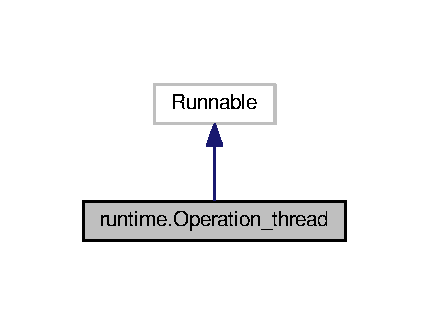
\includegraphics[width=206pt]{classruntime_1_1_operation__thread__inherit__graph}
\end{center}
\end{figure}


Collaboration diagram for runtime.\+Operation\+\_\+thread\+:\nopagebreak
\begin{figure}[H]
\begin{center}
\leavevmode
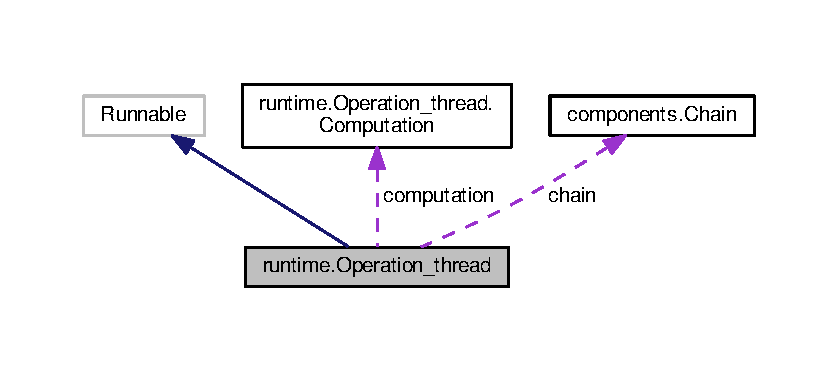
\includegraphics[width=350pt]{classruntime_1_1_operation__thread__coll__graph}
\end{center}
\end{figure}
\subsection*{Classes}
\begin{DoxyCompactItemize}
\item 
enum \hyperlink{enumruntime_1_1_operation__thread_1_1_computation}{Computation}
\end{DoxyCompactItemize}
\subsection*{Public Member Functions}
\begin{DoxyCompactItemize}
\item 
\hyperlink{classruntime_1_1_operation__thread_aa76aa31abd36a7d8af29ae52efba8758}{Operation\+\_\+thread} (\hyperlink{classcomponents_1_1_chain}{Chain} chain, \hyperlink{enumruntime_1_1_operation__thread_1_1_computation}{Computation} computation)
\item 
void \hyperlink{classruntime_1_1_operation__thread_aaee976f90605c4147a8c22bb8f9eee25}{run} ()
\end{DoxyCompactItemize}


\subsection{Detailed Description}
U\+N\+U\+S\+ED. 

The Intent of this class was to run specific computations on a differant thread. It is unused in the current implementation because there is never a need to run one computation independent from the others. 

\subsection{Constructor \& Destructor Documentation}
\index{runtime\+::\+Operation\+\_\+thread@{runtime\+::\+Operation\+\_\+thread}!Operation\+\_\+thread@{Operation\+\_\+thread}}
\index{Operation\+\_\+thread@{Operation\+\_\+thread}!runtime\+::\+Operation\+\_\+thread@{runtime\+::\+Operation\+\_\+thread}}
\subsubsection[{\texorpdfstring{Operation\+\_\+thread(\+Chain chain, Computation computation)}{Operation_thread(Chain chain, Computation computation)}}]{\setlength{\rightskip}{0pt plus 5cm}runtime.\+Operation\+\_\+thread.\+Operation\+\_\+thread (
\begin{DoxyParamCaption}
\item[{{\bf Chain}}]{chain, }
\item[{{\bf Computation}}]{computation}
\end{DoxyParamCaption}
)}\hypertarget{classruntime_1_1_operation__thread_aa76aa31abd36a7d8af29ae52efba8758}{}\label{classruntime_1_1_operation__thread_aa76aa31abd36a7d8af29ae52efba8758}


\subsection{Member Function Documentation}
\index{runtime\+::\+Operation\+\_\+thread@{runtime\+::\+Operation\+\_\+thread}!run@{run}}
\index{run@{run}!runtime\+::\+Operation\+\_\+thread@{runtime\+::\+Operation\+\_\+thread}}
\subsubsection[{\texorpdfstring{run()}{run()}}]{\setlength{\rightskip}{0pt plus 5cm}void runtime.\+Operation\+\_\+thread.\+run (
\begin{DoxyParamCaption}
{}
\end{DoxyParamCaption}
)}\hypertarget{classruntime_1_1_operation__thread_aaee976f90605c4147a8c22bb8f9eee25}{}\label{classruntime_1_1_operation__thread_aaee976f90605c4147a8c22bb8f9eee25}


Here is the call graph for this function\+:\nopagebreak
\begin{figure}[H]
\begin{center}
\leavevmode
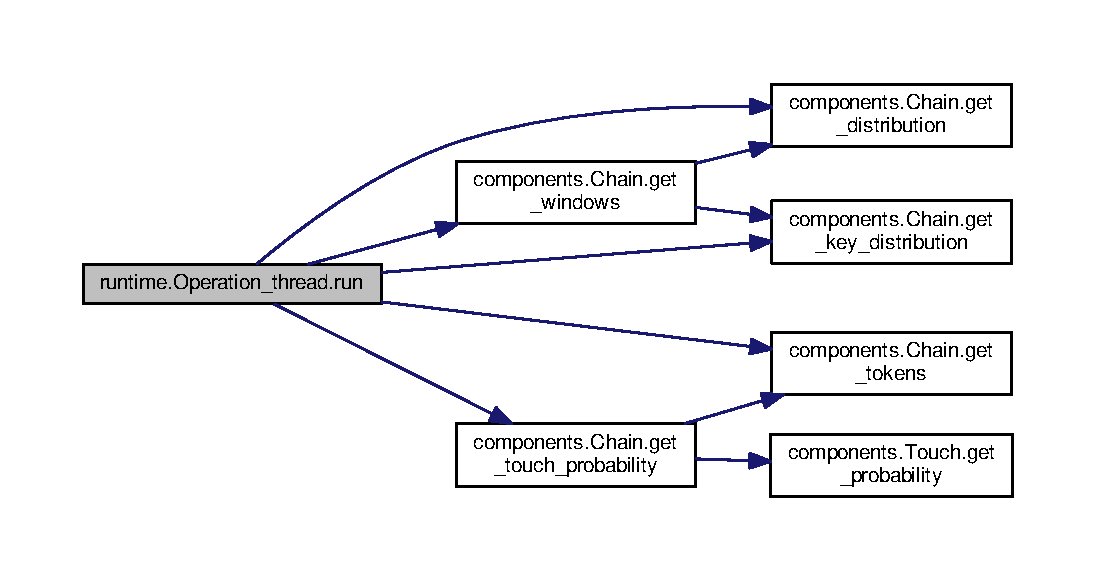
\includegraphics[width=350pt]{classruntime_1_1_operation__thread_aaee976f90605c4147a8c22bb8f9eee25_cgraph}
\end{center}
\end{figure}




The documentation for this class was generated from the following file\+:\begin{DoxyCompactItemize}
\item 
/home/element/\+P\+U\+F/\+Keyboard/java\+\_\+scripts/java\+\_\+marcov\+\_\+model/src/runtime/\hyperlink{_operation__thread_8java}{Operation\+\_\+thread.\+java}\end{DoxyCompactItemize}

\hypertarget{enumtest_1_1_main_1_1_test_files_1_1_pressure_amount}{}\section{test.\+Main.\+Test\+Files.\+Pressure\+Amount Enum Reference}
\label{enumtest_1_1_main_1_1_test_files_1_1_pressure_amount}\index{test.\+Main.\+Test\+Files.\+Pressure\+Amount@{test.\+Main.\+Test\+Files.\+Pressure\+Amount}}
\subsection*{Public Member Functions}
\begin{DoxyCompactItemize}
\item 
\hyperlink{enumtest_1_1_main_1_1_test_files_1_1_pressure_amount_a3bc5a52a8ba8bd7e723bbdf524672511}{Pressure\+Amount} (String description, int identifier, double value)
\item 
String \hyperlink{enumtest_1_1_main_1_1_test_files_1_1_pressure_amount_aea6994ed3f8f7494b72b595a928dd648}{to\+String} ()
\item 
int \hyperlink{enumtest_1_1_main_1_1_test_files_1_1_pressure_amount_adc88b56b134392844a20f9a8fcd73e53}{get\+\_\+identifier} ()
\item 
double \hyperlink{enumtest_1_1_main_1_1_test_files_1_1_pressure_amount_adafeeee7e8e63f9169a03a8555ec685c}{get\+\_\+value} ()
\end{DoxyCompactItemize}
\subsection*{Public Attributes}
\begin{DoxyCompactItemize}
\item 
\hyperlink{enumtest_1_1_main_1_1_test_files_1_1_pressure_amount_a321472c250b974ef4f419acf92300eeb}{H\+I\+GH} =(\char`\"{}High pressure, 0.\+75\char`\"{}, 0, .\+75)
\item 
\hyperlink{enumtest_1_1_main_1_1_test_files_1_1_pressure_amount_a42949a0c635d96edf5eedd231e539e2c}{M\+E\+D\+I\+UM} =(\char`\"{}Medium Pressure, 0.\+5\char`\"{}, 1, .\+5)
\item 
\hyperlink{enumtest_1_1_main_1_1_test_files_1_1_pressure_amount_a7e4af3a5f4b0df871b174b6154903545}{L\+OW}
\end{DoxyCompactItemize}


\subsection{Constructor \& Destructor Documentation}
\index{test\+::\+Main\+::\+Test\+Files\+::\+Pressure\+Amount@{test\+::\+Main\+::\+Test\+Files\+::\+Pressure\+Amount}!Pressure\+Amount@{Pressure\+Amount}}
\index{Pressure\+Amount@{Pressure\+Amount}!test\+::\+Main\+::\+Test\+Files\+::\+Pressure\+Amount@{test\+::\+Main\+::\+Test\+Files\+::\+Pressure\+Amount}}
\subsubsection[{\texorpdfstring{Pressure\+Amount(\+String description, int identifier, double value)}{PressureAmount(String description, int identifier, double value)}}]{\setlength{\rightskip}{0pt plus 5cm}test.\+Main.\+Test\+Files.\+Pressure\+Amount.\+Pressure\+Amount (
\begin{DoxyParamCaption}
\item[{String}]{description, }
\item[{int}]{identifier, }
\item[{double}]{value}
\end{DoxyParamCaption}
)}\hypertarget{enumtest_1_1_main_1_1_test_files_1_1_pressure_amount_a3bc5a52a8ba8bd7e723bbdf524672511}{}\label{enumtest_1_1_main_1_1_test_files_1_1_pressure_amount_a3bc5a52a8ba8bd7e723bbdf524672511}


\subsection{Member Function Documentation}
\index{test\+::\+Main\+::\+Test\+Files\+::\+Pressure\+Amount@{test\+::\+Main\+::\+Test\+Files\+::\+Pressure\+Amount}!get\+\_\+identifier@{get\+\_\+identifier}}
\index{get\+\_\+identifier@{get\+\_\+identifier}!test\+::\+Main\+::\+Test\+Files\+::\+Pressure\+Amount@{test\+::\+Main\+::\+Test\+Files\+::\+Pressure\+Amount}}
\subsubsection[{\texorpdfstring{get\+\_\+identifier()}{get_identifier()}}]{\setlength{\rightskip}{0pt plus 5cm}int test.\+Main.\+Test\+Files.\+Pressure\+Amount.\+get\+\_\+identifier (
\begin{DoxyParamCaption}
{}
\end{DoxyParamCaption}
)}\hypertarget{enumtest_1_1_main_1_1_test_files_1_1_pressure_amount_adc88b56b134392844a20f9a8fcd73e53}{}\label{enumtest_1_1_main_1_1_test_files_1_1_pressure_amount_adc88b56b134392844a20f9a8fcd73e53}
\index{test\+::\+Main\+::\+Test\+Files\+::\+Pressure\+Amount@{test\+::\+Main\+::\+Test\+Files\+::\+Pressure\+Amount}!get\+\_\+value@{get\+\_\+value}}
\index{get\+\_\+value@{get\+\_\+value}!test\+::\+Main\+::\+Test\+Files\+::\+Pressure\+Amount@{test\+::\+Main\+::\+Test\+Files\+::\+Pressure\+Amount}}
\subsubsection[{\texorpdfstring{get\+\_\+value()}{get_value()}}]{\setlength{\rightskip}{0pt plus 5cm}double test.\+Main.\+Test\+Files.\+Pressure\+Amount.\+get\+\_\+value (
\begin{DoxyParamCaption}
{}
\end{DoxyParamCaption}
)}\hypertarget{enumtest_1_1_main_1_1_test_files_1_1_pressure_amount_adafeeee7e8e63f9169a03a8555ec685c}{}\label{enumtest_1_1_main_1_1_test_files_1_1_pressure_amount_adafeeee7e8e63f9169a03a8555ec685c}
\index{test\+::\+Main\+::\+Test\+Files\+::\+Pressure\+Amount@{test\+::\+Main\+::\+Test\+Files\+::\+Pressure\+Amount}!to\+String@{to\+String}}
\index{to\+String@{to\+String}!test\+::\+Main\+::\+Test\+Files\+::\+Pressure\+Amount@{test\+::\+Main\+::\+Test\+Files\+::\+Pressure\+Amount}}
\subsubsection[{\texorpdfstring{to\+String()}{toString()}}]{\setlength{\rightskip}{0pt plus 5cm}String test.\+Main.\+Test\+Files.\+Pressure\+Amount.\+to\+String (
\begin{DoxyParamCaption}
{}
\end{DoxyParamCaption}
)}\hypertarget{enumtest_1_1_main_1_1_test_files_1_1_pressure_amount_aea6994ed3f8f7494b72b595a928dd648}{}\label{enumtest_1_1_main_1_1_test_files_1_1_pressure_amount_aea6994ed3f8f7494b72b595a928dd648}


\subsection{Member Data Documentation}
\index{test\+::\+Main\+::\+Test\+Files\+::\+Pressure\+Amount@{test\+::\+Main\+::\+Test\+Files\+::\+Pressure\+Amount}!H\+I\+GH@{H\+I\+GH}}
\index{H\+I\+GH@{H\+I\+GH}!test\+::\+Main\+::\+Test\+Files\+::\+Pressure\+Amount@{test\+::\+Main\+::\+Test\+Files\+::\+Pressure\+Amount}}
\subsubsection[{\texorpdfstring{H\+I\+GH}{HIGH}}]{\setlength{\rightskip}{0pt plus 5cm}test.\+Main.\+Test\+Files.\+Pressure\+Amount.\+H\+I\+GH =(\char`\"{}High pressure, 0.\+75\char`\"{}, 0, .\+75)}\hypertarget{enumtest_1_1_main_1_1_test_files_1_1_pressure_amount_a321472c250b974ef4f419acf92300eeb}{}\label{enumtest_1_1_main_1_1_test_files_1_1_pressure_amount_a321472c250b974ef4f419acf92300eeb}
\index{test\+::\+Main\+::\+Test\+Files\+::\+Pressure\+Amount@{test\+::\+Main\+::\+Test\+Files\+::\+Pressure\+Amount}!L\+OW@{L\+OW}}
\index{L\+OW@{L\+OW}!test\+::\+Main\+::\+Test\+Files\+::\+Pressure\+Amount@{test\+::\+Main\+::\+Test\+Files\+::\+Pressure\+Amount}}
\subsubsection[{\texorpdfstring{L\+OW}{LOW}}]{\setlength{\rightskip}{0pt plus 5cm}test.\+Main.\+Test\+Files.\+Pressure\+Amount.\+L\+OW}\hypertarget{enumtest_1_1_main_1_1_test_files_1_1_pressure_amount_a7e4af3a5f4b0df871b174b6154903545}{}\label{enumtest_1_1_main_1_1_test_files_1_1_pressure_amount_a7e4af3a5f4b0df871b174b6154903545}
{\bfseries Initial value\+:}
\begin{DoxyCode}
=(\textcolor{stringliteral}{"Low Pressure, 0.25"}, 2,
                    .25)
\end{DoxyCode}
\index{test\+::\+Main\+::\+Test\+Files\+::\+Pressure\+Amount@{test\+::\+Main\+::\+Test\+Files\+::\+Pressure\+Amount}!M\+E\+D\+I\+UM@{M\+E\+D\+I\+UM}}
\index{M\+E\+D\+I\+UM@{M\+E\+D\+I\+UM}!test\+::\+Main\+::\+Test\+Files\+::\+Pressure\+Amount@{test\+::\+Main\+::\+Test\+Files\+::\+Pressure\+Amount}}
\subsubsection[{\texorpdfstring{M\+E\+D\+I\+UM}{MEDIUM}}]{\setlength{\rightskip}{0pt plus 5cm}test.\+Main.\+Test\+Files.\+Pressure\+Amount.\+M\+E\+D\+I\+UM =(\char`\"{}Medium Pressure, 0.\+5\char`\"{}, 1, .\+5)}\hypertarget{enumtest_1_1_main_1_1_test_files_1_1_pressure_amount_a42949a0c635d96edf5eedd231e539e2c}{}\label{enumtest_1_1_main_1_1_test_files_1_1_pressure_amount_a42949a0c635d96edf5eedd231e539e2c}


The documentation for this enum was generated from the following file\+:\begin{DoxyCompactItemize}
\item 
/home/element/\+P\+U\+F/\+Keyboard/java\+\_\+scripts/java\+\_\+marcov\+\_\+model/src/test/\hyperlink{_main_8java}{Main.\+java}\end{DoxyCompactItemize}

\hypertarget{classtest_1_1_print__model}{}\section{test.\+Print\+\_\+model Class Reference}
\label{classtest_1_1_print__model}\index{test.\+Print\+\_\+model@{test.\+Print\+\_\+model}}


This class will print out the model constructed form the designated file.  


\subsection*{Static Public Member Functions}
\begin{DoxyCompactItemize}
\item 
static void \hyperlink{classtest_1_1_print__model_a00a222f0a0350d0d6001a5b722485c1f}{main} (String\mbox{[}$\,$\mbox{]} args)
\end{DoxyCompactItemize}


\subsection{Detailed Description}
This class will print out the model constructed form the designated file. 

\subsection{Member Function Documentation}
\index{test\+::\+Print\+\_\+model@{test\+::\+Print\+\_\+model}!main@{main}}
\index{main@{main}!test\+::\+Print\+\_\+model@{test\+::\+Print\+\_\+model}}
\subsubsection[{\texorpdfstring{main(\+String[] args)}{main(String[] args)}}]{\setlength{\rightskip}{0pt plus 5cm}static void test.\+Print\+\_\+model.\+main (
\begin{DoxyParamCaption}
\item[{String\mbox{[}$\,$\mbox{]}}]{args}
\end{DoxyParamCaption}
)\hspace{0.3cm}{\ttfamily [static]}}\hypertarget{classtest_1_1_print__model_a00a222f0a0350d0d6001a5b722485c1f}{}\label{classtest_1_1_print__model_a00a222f0a0350d0d6001a5b722485c1f}


Here is the call graph for this function\+:\nopagebreak
\begin{figure}[H]
\begin{center}
\leavevmode
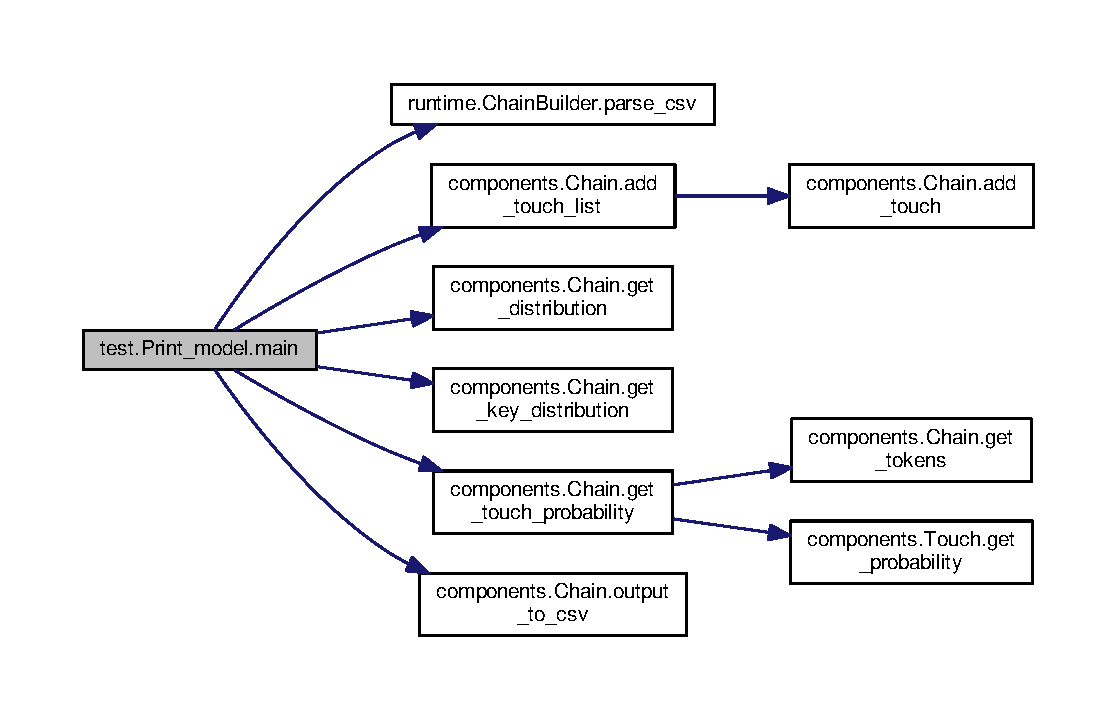
\includegraphics[width=350pt]{classtest_1_1_print__model_a00a222f0a0350d0d6001a5b722485c1f_cgraph}
\end{center}
\end{figure}




Here is the caller graph for this function\+:\nopagebreak
\begin{figure}[H]
\begin{center}
\leavevmode
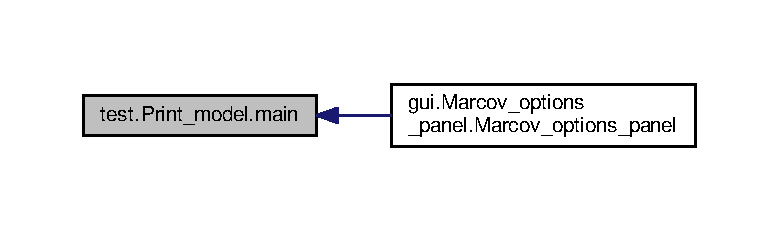
\includegraphics[width=350pt]{classtest_1_1_print__model_a00a222f0a0350d0d6001a5b722485c1f_icgraph}
\end{center}
\end{figure}




The documentation for this class was generated from the following file\+:\begin{DoxyCompactItemize}
\item 
/home/element/\+P\+U\+F/\+Keyboard/java\+\_\+scripts/java\+\_\+marcov\+\_\+model/src/test/\hyperlink{_print__model_8java}{Print\+\_\+model.\+java}\end{DoxyCompactItemize}

\hypertarget{classgui_1_1_start_g_u_i}{}\section{gui.\+Start\+G\+UI Class Reference}
\label{classgui_1_1_start_g_u_i}\index{gui.\+Start\+G\+UI@{gui.\+Start\+G\+UI}}
\subsection*{Static Public Member Functions}
\begin{DoxyCompactItemize}
\item 
static void \hyperlink{classgui_1_1_start_g_u_i_a8b6034c18fed02e227497a3c6e188f12}{main} (String\mbox{[}$\,$\mbox{]} args)
\item 
static void \hyperlink{classgui_1_1_start_g_u_i_a92880df89c85411e12e66594bc0c011d}{exit} ()
\begin{DoxyCompactList}\small\item\em causes the frame to close \end{DoxyCompactList}\end{DoxyCompactItemize}


\subsection{Member Function Documentation}
\index{gui\+::\+Start\+G\+UI@{gui\+::\+Start\+G\+UI}!exit@{exit}}
\index{exit@{exit}!gui\+::\+Start\+G\+UI@{gui\+::\+Start\+G\+UI}}
\subsubsection[{\texorpdfstring{exit()}{exit()}}]{\setlength{\rightskip}{0pt plus 5cm}static void gui.\+Start\+G\+U\+I.\+exit (
\begin{DoxyParamCaption}
{}
\end{DoxyParamCaption}
)\hspace{0.3cm}{\ttfamily [static]}}\hypertarget{classgui_1_1_start_g_u_i_a92880df89c85411e12e66594bc0c011d}{}\label{classgui_1_1_start_g_u_i_a92880df89c85411e12e66594bc0c011d}


causes the frame to close 

\index{gui\+::\+Start\+G\+UI@{gui\+::\+Start\+G\+UI}!main@{main}}
\index{main@{main}!gui\+::\+Start\+G\+UI@{gui\+::\+Start\+G\+UI}}
\subsubsection[{\texorpdfstring{main(\+String[] args)}{main(String[] args)}}]{\setlength{\rightskip}{0pt plus 5cm}static void gui.\+Start\+G\+U\+I.\+main (
\begin{DoxyParamCaption}
\item[{String\mbox{[}$\,$\mbox{]}}]{args}
\end{DoxyParamCaption}
)\hspace{0.3cm}{\ttfamily [static]}}\hypertarget{classgui_1_1_start_g_u_i_a8b6034c18fed02e227497a3c6e188f12}{}\label{classgui_1_1_start_g_u_i_a8b6034c18fed02e227497a3c6e188f12}


The documentation for this class was generated from the following file\+:\begin{DoxyCompactItemize}
\item 
/home/element/\+P\+U\+F/\+Keyboard/java\+\_\+scripts/java\+\_\+marcov\+\_\+model/src/gui/\hyperlink{_start_g_u_i_8java}{Start\+G\+U\+I.\+java}\end{DoxyCompactItemize}

\hypertarget{enumruntime_1_1_chain_builder_1_1_state}{}\section{runtime.\+Chain\+Builder.\+State Enum Reference}
\label{enumruntime_1_1_chain_builder_1_1_state}\index{runtime.\+Chain\+Builder.\+State@{runtime.\+Chain\+Builder.\+State}}
\subsection*{Public Attributes}
\begin{DoxyCompactItemize}
\item 
\hyperlink{enumruntime_1_1_chain_builder_1_1_state_a62c8f060cacdb5e4e00cfd49eb589256}{I\+N\+\_\+\+P\+R\+O\+G\+R\+E\+SS}
\item 
\hyperlink{enumruntime_1_1_chain_builder_1_1_state_a4e4251132b0507e126673689e1f01b7a}{S\+U\+C\+C\+E\+SS}
\end{DoxyCompactItemize}


\subsection{Member Data Documentation}
\index{runtime\+::\+Chain\+Builder\+::\+State@{runtime\+::\+Chain\+Builder\+::\+State}!I\+N\+\_\+\+P\+R\+O\+G\+R\+E\+SS@{I\+N\+\_\+\+P\+R\+O\+G\+R\+E\+SS}}
\index{I\+N\+\_\+\+P\+R\+O\+G\+R\+E\+SS@{I\+N\+\_\+\+P\+R\+O\+G\+R\+E\+SS}!runtime\+::\+Chain\+Builder\+::\+State@{runtime\+::\+Chain\+Builder\+::\+State}}
\subsubsection[{\texorpdfstring{I\+N\+\_\+\+P\+R\+O\+G\+R\+E\+SS}{IN_PROGRESS}}]{\setlength{\rightskip}{0pt plus 5cm}runtime.\+Chain\+Builder.\+State.\+I\+N\+\_\+\+P\+R\+O\+G\+R\+E\+SS}\hypertarget{enumruntime_1_1_chain_builder_1_1_state_a62c8f060cacdb5e4e00cfd49eb589256}{}\label{enumruntime_1_1_chain_builder_1_1_state_a62c8f060cacdb5e4e00cfd49eb589256}
\index{runtime\+::\+Chain\+Builder\+::\+State@{runtime\+::\+Chain\+Builder\+::\+State}!S\+U\+C\+C\+E\+SS@{S\+U\+C\+C\+E\+SS}}
\index{S\+U\+C\+C\+E\+SS@{S\+U\+C\+C\+E\+SS}!runtime\+::\+Chain\+Builder\+::\+State@{runtime\+::\+Chain\+Builder\+::\+State}}
\subsubsection[{\texorpdfstring{S\+U\+C\+C\+E\+SS}{SUCCESS}}]{\setlength{\rightskip}{0pt plus 5cm}runtime.\+Chain\+Builder.\+State.\+S\+U\+C\+C\+E\+SS}\hypertarget{enumruntime_1_1_chain_builder_1_1_state_a4e4251132b0507e126673689e1f01b7a}{}\label{enumruntime_1_1_chain_builder_1_1_state_a4e4251132b0507e126673689e1f01b7a}


The documentation for this enum was generated from the following file\+:\begin{DoxyCompactItemize}
\item 
/home/element/\+P\+U\+F/\+Keyboard/java\+\_\+scripts/java\+\_\+marcov\+\_\+model/src/runtime/\hyperlink{_chain_builder_8java}{Chain\+Builder.\+java}\end{DoxyCompactItemize}

\hypertarget{classdata__analysis_1_1_statistics}{}\section{data\+\_\+analysis.\+Statistics Class Reference}
\label{classdata__analysis_1_1_statistics}\index{data\+\_\+analysis.\+Statistics@{data\+\_\+analysis.\+Statistics}}
\subsection*{Static Public Member Functions}
\begin{DoxyCompactItemize}
\item 
static void \hyperlink{classdata__analysis_1_1_statistics_a19371eed8cab72da351f6c35762c83de}{main} (String args\mbox{[}$\,$\mbox{]})
\item 
static double \hyperlink{classdata__analysis_1_1_statistics_a0c7f157e53361c33276290383acff9b6}{false\+\_\+positive\+\_\+percentage} (double authentication\+\_\+percentage, List$<$ Double $>$ should\+\_\+authenticate\+\_\+percentages, List$<$ Double $>$ should\+\_\+not\+\_\+authenticate\+\_\+percentages)
\item 
static double \hyperlink{classdata__analysis_1_1_statistics_abcd420f8186babaf12e030180e4c458d}{false\+\_\+negative\+\_\+percentage} (double authentication\+\_\+percentage, List$<$ Double $>$ should\+\_\+authenticate\+\_\+percentages, List$<$ Double $>$ should\+\_\+not\+\_\+authenticate\+\_\+percentages)
\item 
static double \hyperlink{classdata__analysis_1_1_statistics_afb383973976b2531318be692c4894f5e}{best\+\_\+authentication\+\_\+percentage} (List$<$ Double $>$ should\+\_\+authenticate\+\_\+percentages, List$<$ Double $>$ should\+\_\+not\+\_\+authenticate\+\_\+percentages)
\item 
static double \hyperlink{classdata__analysis_1_1_statistics_a4fff292245c5c2435386e12b129c2b40}{minimize\+\_\+false\+\_\+positive\+\_\+authentication\+\_\+percentage} (List$<$ Double $>$ should\+\_\+authenticate\+\_\+percentages, List$<$ Double $>$ should\+\_\+not\+\_\+authenticate\+\_\+percentages)
\item 
static double \hyperlink{classdata__analysis_1_1_statistics_a7702c206ace91fa095d5b68a24820db2}{equal\+\_\+false\+\_\+positive\+\_\+negative\+\_\+authentication\+\_\+percentage} (List$<$ Double $>$ should\+\_\+authenticate\+\_\+percentages, List$<$ Double $>$ should\+\_\+not\+\_\+authenticate\+\_\+percentages)
\item 
static double \hyperlink{classdata__analysis_1_1_statistics_a8ca0530f61c30cf41f0500e56b6fc11a}{authentication\+\_\+accuracy} (double authentication\+\_\+percentage, List$<$ Double $>$ should\+\_\+authenticate\+\_\+percentages, List$<$ Double $>$ should\+\_\+not\+\_\+authenticate\+\_\+percentages)
\end{DoxyCompactItemize}


\subsection{Member Function Documentation}
\index{data\+\_\+analysis\+::\+Statistics@{data\+\_\+analysis\+::\+Statistics}!authentication\+\_\+accuracy@{authentication\+\_\+accuracy}}
\index{authentication\+\_\+accuracy@{authentication\+\_\+accuracy}!data\+\_\+analysis\+::\+Statistics@{data\+\_\+analysis\+::\+Statistics}}
\subsubsection[{\texorpdfstring{authentication\+\_\+accuracy(double authentication\+\_\+percentage, List$<$ Double $>$ should\+\_\+authenticate\+\_\+percentages, List$<$ Double $>$ should\+\_\+not\+\_\+authenticate\+\_\+percentages)}{authentication_accuracy(double authentication_percentage, List< Double > should_authenticate_percentages, List< Double > should_not_authenticate_percentages)}}]{\setlength{\rightskip}{0pt plus 5cm}static double data\+\_\+analysis.\+Statistics.\+authentication\+\_\+accuracy (
\begin{DoxyParamCaption}
\item[{double}]{authentication\+\_\+percentage, }
\item[{List$<$ Double $>$}]{should\+\_\+authenticate\+\_\+percentages, }
\item[{List$<$ Double $>$}]{should\+\_\+not\+\_\+authenticate\+\_\+percentages}
\end{DoxyParamCaption}
)\hspace{0.3cm}{\ttfamily [static]}}\hypertarget{classdata__analysis_1_1_statistics_a8ca0530f61c30cf41f0500e56b6fc11a}{}\label{classdata__analysis_1_1_statistics_a8ca0530f61c30cf41f0500e56b6fc11a}
\index{data\+\_\+analysis\+::\+Statistics@{data\+\_\+analysis\+::\+Statistics}!best\+\_\+authentication\+\_\+percentage@{best\+\_\+authentication\+\_\+percentage}}
\index{best\+\_\+authentication\+\_\+percentage@{best\+\_\+authentication\+\_\+percentage}!data\+\_\+analysis\+::\+Statistics@{data\+\_\+analysis\+::\+Statistics}}
\subsubsection[{\texorpdfstring{best\+\_\+authentication\+\_\+percentage(\+List$<$ Double $>$ should\+\_\+authenticate\+\_\+percentages, List$<$ Double $>$ should\+\_\+not\+\_\+authenticate\+\_\+percentages)}{best_authentication_percentage(List< Double > should_authenticate_percentages, List< Double > should_not_authenticate_percentages)}}]{\setlength{\rightskip}{0pt plus 5cm}static double data\+\_\+analysis.\+Statistics.\+best\+\_\+authentication\+\_\+percentage (
\begin{DoxyParamCaption}
\item[{List$<$ Double $>$}]{should\+\_\+authenticate\+\_\+percentages, }
\item[{List$<$ Double $>$}]{should\+\_\+not\+\_\+authenticate\+\_\+percentages}
\end{DoxyParamCaption}
)\hspace{0.3cm}{\ttfamily [static]}}\hypertarget{classdata__analysis_1_1_statistics_afb383973976b2531318be692c4894f5e}{}\label{classdata__analysis_1_1_statistics_afb383973976b2531318be692c4894f5e}
\index{data\+\_\+analysis\+::\+Statistics@{data\+\_\+analysis\+::\+Statistics}!equal\+\_\+false\+\_\+positive\+\_\+negative\+\_\+authentication\+\_\+percentage@{equal\+\_\+false\+\_\+positive\+\_\+negative\+\_\+authentication\+\_\+percentage}}
\index{equal\+\_\+false\+\_\+positive\+\_\+negative\+\_\+authentication\+\_\+percentage@{equal\+\_\+false\+\_\+positive\+\_\+negative\+\_\+authentication\+\_\+percentage}!data\+\_\+analysis\+::\+Statistics@{data\+\_\+analysis\+::\+Statistics}}
\subsubsection[{\texorpdfstring{equal\+\_\+false\+\_\+positive\+\_\+negative\+\_\+authentication\+\_\+percentage(\+List$<$ Double $>$ should\+\_\+authenticate\+\_\+percentages, List$<$ Double $>$ should\+\_\+not\+\_\+authenticate\+\_\+percentages)}{equal_false_positive_negative_authentication_percentage(List< Double > should_authenticate_percentages, List< Double > should_not_authenticate_percentages)}}]{\setlength{\rightskip}{0pt plus 5cm}static double data\+\_\+analysis.\+Statistics.\+equal\+\_\+false\+\_\+positive\+\_\+negative\+\_\+authentication\+\_\+percentage (
\begin{DoxyParamCaption}
\item[{List$<$ Double $>$}]{should\+\_\+authenticate\+\_\+percentages, }
\item[{List$<$ Double $>$}]{should\+\_\+not\+\_\+authenticate\+\_\+percentages}
\end{DoxyParamCaption}
)\hspace{0.3cm}{\ttfamily [static]}}\hypertarget{classdata__analysis_1_1_statistics_a7702c206ace91fa095d5b68a24820db2}{}\label{classdata__analysis_1_1_statistics_a7702c206ace91fa095d5b68a24820db2}
\index{data\+\_\+analysis\+::\+Statistics@{data\+\_\+analysis\+::\+Statistics}!false\+\_\+negative\+\_\+percentage@{false\+\_\+negative\+\_\+percentage}}
\index{false\+\_\+negative\+\_\+percentage@{false\+\_\+negative\+\_\+percentage}!data\+\_\+analysis\+::\+Statistics@{data\+\_\+analysis\+::\+Statistics}}
\subsubsection[{\texorpdfstring{false\+\_\+negative\+\_\+percentage(double authentication\+\_\+percentage, List$<$ Double $>$ should\+\_\+authenticate\+\_\+percentages, List$<$ Double $>$ should\+\_\+not\+\_\+authenticate\+\_\+percentages)}{false_negative_percentage(double authentication_percentage, List< Double > should_authenticate_percentages, List< Double > should_not_authenticate_percentages)}}]{\setlength{\rightskip}{0pt plus 5cm}static double data\+\_\+analysis.\+Statistics.\+false\+\_\+negative\+\_\+percentage (
\begin{DoxyParamCaption}
\item[{double}]{authentication\+\_\+percentage, }
\item[{List$<$ Double $>$}]{should\+\_\+authenticate\+\_\+percentages, }
\item[{List$<$ Double $>$}]{should\+\_\+not\+\_\+authenticate\+\_\+percentages}
\end{DoxyParamCaption}
)\hspace{0.3cm}{\ttfamily [static]}}\hypertarget{classdata__analysis_1_1_statistics_abcd420f8186babaf12e030180e4c458d}{}\label{classdata__analysis_1_1_statistics_abcd420f8186babaf12e030180e4c458d}
\index{data\+\_\+analysis\+::\+Statistics@{data\+\_\+analysis\+::\+Statistics}!false\+\_\+positive\+\_\+percentage@{false\+\_\+positive\+\_\+percentage}}
\index{false\+\_\+positive\+\_\+percentage@{false\+\_\+positive\+\_\+percentage}!data\+\_\+analysis\+::\+Statistics@{data\+\_\+analysis\+::\+Statistics}}
\subsubsection[{\texorpdfstring{false\+\_\+positive\+\_\+percentage(double authentication\+\_\+percentage, List$<$ Double $>$ should\+\_\+authenticate\+\_\+percentages, List$<$ Double $>$ should\+\_\+not\+\_\+authenticate\+\_\+percentages)}{false_positive_percentage(double authentication_percentage, List< Double > should_authenticate_percentages, List< Double > should_not_authenticate_percentages)}}]{\setlength{\rightskip}{0pt plus 5cm}static double data\+\_\+analysis.\+Statistics.\+false\+\_\+positive\+\_\+percentage (
\begin{DoxyParamCaption}
\item[{double}]{authentication\+\_\+percentage, }
\item[{List$<$ Double $>$}]{should\+\_\+authenticate\+\_\+percentages, }
\item[{List$<$ Double $>$}]{should\+\_\+not\+\_\+authenticate\+\_\+percentages}
\end{DoxyParamCaption}
)\hspace{0.3cm}{\ttfamily [static]}}\hypertarget{classdata__analysis_1_1_statistics_a0c7f157e53361c33276290383acff9b6}{}\label{classdata__analysis_1_1_statistics_a0c7f157e53361c33276290383acff9b6}
\index{data\+\_\+analysis\+::\+Statistics@{data\+\_\+analysis\+::\+Statistics}!main@{main}}
\index{main@{main}!data\+\_\+analysis\+::\+Statistics@{data\+\_\+analysis\+::\+Statistics}}
\subsubsection[{\texorpdfstring{main(\+String args[])}{main(String args[])}}]{\setlength{\rightskip}{0pt plus 5cm}static void data\+\_\+analysis.\+Statistics.\+main (
\begin{DoxyParamCaption}
\item[{String}]{args\mbox{[}$\,$\mbox{]}}
\end{DoxyParamCaption}
)\hspace{0.3cm}{\ttfamily [static]}}\hypertarget{classdata__analysis_1_1_statistics_a19371eed8cab72da351f6c35762c83de}{}\label{classdata__analysis_1_1_statistics_a19371eed8cab72da351f6c35762c83de}
\index{data\+\_\+analysis\+::\+Statistics@{data\+\_\+analysis\+::\+Statistics}!minimize\+\_\+false\+\_\+positive\+\_\+authentication\+\_\+percentage@{minimize\+\_\+false\+\_\+positive\+\_\+authentication\+\_\+percentage}}
\index{minimize\+\_\+false\+\_\+positive\+\_\+authentication\+\_\+percentage@{minimize\+\_\+false\+\_\+positive\+\_\+authentication\+\_\+percentage}!data\+\_\+analysis\+::\+Statistics@{data\+\_\+analysis\+::\+Statistics}}
\subsubsection[{\texorpdfstring{minimize\+\_\+false\+\_\+positive\+\_\+authentication\+\_\+percentage(\+List$<$ Double $>$ should\+\_\+authenticate\+\_\+percentages, List$<$ Double $>$ should\+\_\+not\+\_\+authenticate\+\_\+percentages)}{minimize_false_positive_authentication_percentage(List< Double > should_authenticate_percentages, List< Double > should_not_authenticate_percentages)}}]{\setlength{\rightskip}{0pt plus 5cm}static double data\+\_\+analysis.\+Statistics.\+minimize\+\_\+false\+\_\+positive\+\_\+authentication\+\_\+percentage (
\begin{DoxyParamCaption}
\item[{List$<$ Double $>$}]{should\+\_\+authenticate\+\_\+percentages, }
\item[{List$<$ Double $>$}]{should\+\_\+not\+\_\+authenticate\+\_\+percentages}
\end{DoxyParamCaption}
)\hspace{0.3cm}{\ttfamily [static]}}\hypertarget{classdata__analysis_1_1_statistics_a4fff292245c5c2435386e12b129c2b40}{}\label{classdata__analysis_1_1_statistics_a4fff292245c5c2435386e12b129c2b40}


The documentation for this class was generated from the following file\+:\begin{DoxyCompactItemize}
\item 
/home/element/\+P\+U\+F/\+Keyboard/java\+\_\+scripts/java\+\_\+marcov\+\_\+model/src/data\+\_\+analysis/\hyperlink{_statistics_8java}{Statistics.\+java}\end{DoxyCompactItemize}

\hypertarget{classcomponents_1_1_token}{}\section{components.\+Token Class Reference}
\label{classcomponents_1_1_token}\index{components.\+Token@{components.\+Token}}
\subsection*{Classes}
\begin{DoxyCompactItemize}
\item 
enum \hyperlink{enumcomponents_1_1_token_1_1_type}{Type}
\begin{DoxyCompactList}\small\item\em specify the type of token we want to build \end{DoxyCompactList}\end{DoxyCompactItemize}
\subsection*{Public Member Functions}
\begin{DoxyCompactItemize}
\item 
\hyperlink{classcomponents_1_1_token_a73f5eb6dda64ee3049237ca34f28a73c}{Token} (\hyperlink{classcomponents_1_1_distribution}{Distribution} distribution, int total\+\_\+tokens, int token\+\_\+index, double standard\+\_\+deviations, \hyperlink{enumcomponents_1_1_token_1_1_type}{Type} type)
\begin{DoxyCompactList}\small\item\em allow tokens to be created making each touch mu for its keycode, or in a linear fashion over the distribution for the keycode \end{DoxyCompactList}\item 
\hyperlink{classcomponents_1_1_token_aaecd79f21bdfa6dd838719b4cf736df0}{Token} (\hyperlink{classcomponents_1_1_distribution}{Distribution} distribution, int total\+\_\+tokens, int token\+\_\+index, \hyperlink{enumcomponents_1_1_token_1_1_type}{Type} type)
\begin{DoxyCompactList}\small\item\em allow for creation of tokens over a distribution \end{DoxyCompactList}\item 
\hyperlink{classcomponents_1_1_token_aec989a1d1fd6f860a84839091bf0586a}{Token} (double range\+\_\+min, double range\+\_\+max, int total\+\_\+tokens, int token\+\_\+index, \hyperlink{enumcomponents_1_1_token_1_1_type}{Type} type)
\item 
boolean \hyperlink{classcomponents_1_1_token_af023f6e27fd68da7705603161ccffe36}{contains} (\hyperlink{classcomponents_1_1_touch}{Touch} touch)
\item 
boolean \hyperlink{classcomponents_1_1_token_a3e7b6d12602ff4da363a96701e2a365f}{is\+\_\+high\+\_\+wildcard} (\hyperlink{classcomponents_1_1_touch}{Touch} touch)
\begin{DoxyCompactList}\small\item\em determine if a touch is a high\+\_\+wildcard \end{DoxyCompactList}\item 
boolean \hyperlink{classcomponents_1_1_token_a5e1eeb68449d6a940302f6b2561c6cec}{is\+\_\+low\+\_\+wildcard} (\hyperlink{classcomponents_1_1_touch}{Touch} touch)
\begin{DoxyCompactList}\small\item\em determine if a touch is a low wildcard \end{DoxyCompactList}\item 
void \hyperlink{classcomponents_1_1_token_adb18305be1ee0eb86e7a27b59d62a3ab}{increment\+\_\+high\+\_\+wildcards} ()
\begin{DoxyCompactList}\small\item\em adds the the number of high wildcards \end{DoxyCompactList}\item 
void \hyperlink{classcomponents_1_1_token_aedf81a3bafbf9843754192a5f287a06d}{increment\+\_\+low\+\_\+wildcards} ()
\begin{DoxyCompactList}\small\item\em adds the the number of high wildcards \end{DoxyCompactList}\item 
int \hyperlink{classcomponents_1_1_token_a08348f7ec1a53d80f8886cca07e70e97}{get\+\_\+total\+\_\+wildcards} ()
\begin{DoxyCompactList}\small\item\em returns the total number of wildcards \end{DoxyCompactList}\item 
int \hyperlink{classcomponents_1_1_token_a1f4fc1f480c23dcd8bc00a43b34ed613}{get\+\_\+acceptable\+\_\+wildcards} (int total\+\_\+items)
\item 
double \hyperlink{classcomponents_1_1_token_a7139374ae5d36699d9d0b2e80d9afde7}{get\+\_\+min} ()
\begin{DoxyCompactList}\small\item\em returns true if there are more than an acceptable number of wildcards \end{DoxyCompactList}\item 
double \hyperlink{classcomponents_1_1_token_a200e957fcc13ec21353edc5e4510cf67}{get\+\_\+max} ()
\begin{DoxyCompactList}\small\item\em return the maximum \end{DoxyCompactList}\item 
boolean \hyperlink{classcomponents_1_1_token_a9d029725d9c98ef58017aee36be0989d}{equals} (Object o\+\_\+t)
\begin{DoxyCompactList}\small\item\em compares This token to another to determine if they are the same \end{DoxyCompactList}\end{DoxyCompactItemize}


\subsection{Detailed Description}
This class represents a token within the model. Essentially this is a range of values. A touch is defined to be within a token if the pressure value of the touch falls within this range. This class is designed to abstract away the clustering algorithm. This makes the rest of the code far simpler to think about Something to look at in the future may be a clustering algorithm that is not equally distributed 

\subsection{Constructor \& Destructor Documentation}
\index{components\+::\+Token@{components\+::\+Token}!Token@{Token}}
\index{Token@{Token}!components\+::\+Token@{components\+::\+Token}}
\subsubsection[{\texorpdfstring{Token(\+Distribution distribution, int total\+\_\+tokens, int token\+\_\+index, double standard\+\_\+deviations, Type type)}{Token(Distribution distribution, int total_tokens, int token_index, double standard_deviations, Type type)}}]{\setlength{\rightskip}{0pt plus 5cm}components.\+Token.\+Token (
\begin{DoxyParamCaption}
\item[{{\bf Distribution}}]{distribution, }
\item[{int}]{total\+\_\+tokens, }
\item[{int}]{token\+\_\+index, }
\item[{double}]{standard\+\_\+deviations, }
\item[{{\bf Type}}]{type}
\end{DoxyParamCaption}
)}\hypertarget{classcomponents_1_1_token_a73f5eb6dda64ee3049237ca34f28a73c}{}\label{classcomponents_1_1_token_a73f5eb6dda64ee3049237ca34f28a73c}


allow tokens to be created making each touch mu for its keycode, or in a linear fashion over the distribution for the keycode 

allow for creation of tokens with-\/in some number of standard deviations of a distribution \index{components\+::\+Token@{components\+::\+Token}!Token@{Token}}
\index{Token@{Token}!components\+::\+Token@{components\+::\+Token}}
\subsubsection[{\texorpdfstring{Token(\+Distribution distribution, int total\+\_\+tokens, int token\+\_\+index, Type type)}{Token(Distribution distribution, int total_tokens, int token_index, Type type)}}]{\setlength{\rightskip}{0pt plus 5cm}components.\+Token.\+Token (
\begin{DoxyParamCaption}
\item[{{\bf Distribution}}]{distribution, }
\item[{int}]{total\+\_\+tokens, }
\item[{int}]{token\+\_\+index, }
\item[{{\bf Type}}]{type}
\end{DoxyParamCaption}
)}\hypertarget{classcomponents_1_1_token_aaecd79f21bdfa6dd838719b4cf736df0}{}\label{classcomponents_1_1_token_aaecd79f21bdfa6dd838719b4cf736df0}


allow for creation of tokens over a distribution 

\index{components\+::\+Token@{components\+::\+Token}!Token@{Token}}
\index{Token@{Token}!components\+::\+Token@{components\+::\+Token}}
\subsubsection[{\texorpdfstring{Token(double range\+\_\+min, double range\+\_\+max, int total\+\_\+tokens, int token\+\_\+index, Type type)}{Token(double range_min, double range_max, int total_tokens, int token_index, Type type)}}]{\setlength{\rightskip}{0pt plus 5cm}components.\+Token.\+Token (
\begin{DoxyParamCaption}
\item[{double}]{range\+\_\+min, }
\item[{double}]{range\+\_\+max, }
\item[{int}]{total\+\_\+tokens, }
\item[{int}]{token\+\_\+index, }
\item[{{\bf Type}}]{type}
\end{DoxyParamCaption}
)}\hypertarget{classcomponents_1_1_token_aec989a1d1fd6f860a84839091bf0586a}{}\label{classcomponents_1_1_token_aec989a1d1fd6f860a84839091bf0586a}
Implemented in the constructor is the clustering algorithm. This determines how to split up the range into a number of tokens.

range\+\_\+min, minimum of the token range range\+\_\+max, maximum of the token range total\+\_\+tokens total number of tokens to split range into token\+\_\+index, integer between 0 and total\+\_\+tokens-\/1 indicating into which range this token falls 

\subsection{Member Function Documentation}
\index{components\+::\+Token@{components\+::\+Token}!contains@{contains}}
\index{contains@{contains}!components\+::\+Token@{components\+::\+Token}}
\subsubsection[{\texorpdfstring{contains(\+Touch touch)}{contains(Touch touch)}}]{\setlength{\rightskip}{0pt plus 5cm}boolean components.\+Token.\+contains (
\begin{DoxyParamCaption}
\item[{{\bf Touch}}]{touch}
\end{DoxyParamCaption}
)}\hypertarget{classcomponents_1_1_token_af023f6e27fd68da7705603161ccffe36}{}\label{classcomponents_1_1_token_af023f6e27fd68da7705603161ccffe36}
determines if a touch is within this token based on its pressure value this will return true if a touches pressure equals max or min, so if max of one token is min of another token, both will return true \index{components\+::\+Token@{components\+::\+Token}!equals@{equals}}
\index{equals@{equals}!components\+::\+Token@{components\+::\+Token}}
\subsubsection[{\texorpdfstring{equals(\+Object o\+\_\+t)}{equals(Object o_t)}}]{\setlength{\rightskip}{0pt plus 5cm}boolean components.\+Token.\+equals (
\begin{DoxyParamCaption}
\item[{Object}]{o\+\_\+t}
\end{DoxyParamCaption}
)}\hypertarget{classcomponents_1_1_token_a9d029725d9c98ef58017aee36be0989d}{}\label{classcomponents_1_1_token_a9d029725d9c98ef58017aee36be0989d}


compares This token to another to determine if they are the same 

\index{components\+::\+Token@{components\+::\+Token}!get\+\_\+acceptable\+\_\+wildcards@{get\+\_\+acceptable\+\_\+wildcards}}
\index{get\+\_\+acceptable\+\_\+wildcards@{get\+\_\+acceptable\+\_\+wildcards}!components\+::\+Token@{components\+::\+Token}}
\subsubsection[{\texorpdfstring{get\+\_\+acceptable\+\_\+wildcards(int total\+\_\+items)}{get_acceptable_wildcards(int total_items)}}]{\setlength{\rightskip}{0pt plus 5cm}int components.\+Token.\+get\+\_\+acceptable\+\_\+wildcards (
\begin{DoxyParamCaption}
\item[{int}]{total\+\_\+items}
\end{DoxyParamCaption}
)}\hypertarget{classcomponents_1_1_token_a1f4fc1f480c23dcd8bc00a43b34ed613}{}\label{classcomponents_1_1_token_a1f4fc1f480c23dcd8bc00a43b34ed613}
returns the acceptable number of wildcards 
\begin{DoxyParams}{Parameters}
{\em total\+\_\+items} & is the total number of items in the distribution \\
\hline
\end{DoxyParams}
\index{components\+::\+Token@{components\+::\+Token}!get\+\_\+max@{get\+\_\+max}}
\index{get\+\_\+max@{get\+\_\+max}!components\+::\+Token@{components\+::\+Token}}
\subsubsection[{\texorpdfstring{get\+\_\+max()}{get_max()}}]{\setlength{\rightskip}{0pt plus 5cm}double components.\+Token.\+get\+\_\+max (
\begin{DoxyParamCaption}
{}
\end{DoxyParamCaption}
)}\hypertarget{classcomponents_1_1_token_a200e957fcc13ec21353edc5e4510cf67}{}\label{classcomponents_1_1_token_a200e957fcc13ec21353edc5e4510cf67}


return the maximum 

\index{components\+::\+Token@{components\+::\+Token}!get\+\_\+min@{get\+\_\+min}}
\index{get\+\_\+min@{get\+\_\+min}!components\+::\+Token@{components\+::\+Token}}
\subsubsection[{\texorpdfstring{get\+\_\+min()}{get_min()}}]{\setlength{\rightskip}{0pt plus 5cm}double components.\+Token.\+get\+\_\+min (
\begin{DoxyParamCaption}
{}
\end{DoxyParamCaption}
)}\hypertarget{classcomponents_1_1_token_a7139374ae5d36699d9d0b2e80d9afde7}{}\label{classcomponents_1_1_token_a7139374ae5d36699d9d0b2e80d9afde7}


returns true if there are more than an acceptable number of wildcards 

return minimum \index{components\+::\+Token@{components\+::\+Token}!get\+\_\+total\+\_\+wildcards@{get\+\_\+total\+\_\+wildcards}}
\index{get\+\_\+total\+\_\+wildcards@{get\+\_\+total\+\_\+wildcards}!components\+::\+Token@{components\+::\+Token}}
\subsubsection[{\texorpdfstring{get\+\_\+total\+\_\+wildcards()}{get_total_wildcards()}}]{\setlength{\rightskip}{0pt plus 5cm}int components.\+Token.\+get\+\_\+total\+\_\+wildcards (
\begin{DoxyParamCaption}
{}
\end{DoxyParamCaption}
)}\hypertarget{classcomponents_1_1_token_a08348f7ec1a53d80f8886cca07e70e97}{}\label{classcomponents_1_1_token_a08348f7ec1a53d80f8886cca07e70e97}


returns the total number of wildcards 

\index{components\+::\+Token@{components\+::\+Token}!increment\+\_\+high\+\_\+wildcards@{increment\+\_\+high\+\_\+wildcards}}
\index{increment\+\_\+high\+\_\+wildcards@{increment\+\_\+high\+\_\+wildcards}!components\+::\+Token@{components\+::\+Token}}
\subsubsection[{\texorpdfstring{increment\+\_\+high\+\_\+wildcards()}{increment_high_wildcards()}}]{\setlength{\rightskip}{0pt plus 5cm}void components.\+Token.\+increment\+\_\+high\+\_\+wildcards (
\begin{DoxyParamCaption}
{}
\end{DoxyParamCaption}
)}\hypertarget{classcomponents_1_1_token_adb18305be1ee0eb86e7a27b59d62a3ab}{}\label{classcomponents_1_1_token_adb18305be1ee0eb86e7a27b59d62a3ab}


adds the the number of high wildcards 

\index{components\+::\+Token@{components\+::\+Token}!increment\+\_\+low\+\_\+wildcards@{increment\+\_\+low\+\_\+wildcards}}
\index{increment\+\_\+low\+\_\+wildcards@{increment\+\_\+low\+\_\+wildcards}!components\+::\+Token@{components\+::\+Token}}
\subsubsection[{\texorpdfstring{increment\+\_\+low\+\_\+wildcards()}{increment_low_wildcards()}}]{\setlength{\rightskip}{0pt plus 5cm}void components.\+Token.\+increment\+\_\+low\+\_\+wildcards (
\begin{DoxyParamCaption}
{}
\end{DoxyParamCaption}
)}\hypertarget{classcomponents_1_1_token_aedf81a3bafbf9843754192a5f287a06d}{}\label{classcomponents_1_1_token_aedf81a3bafbf9843754192a5f287a06d}


adds the the number of high wildcards 

\index{components\+::\+Token@{components\+::\+Token}!is\+\_\+high\+\_\+wildcard@{is\+\_\+high\+\_\+wildcard}}
\index{is\+\_\+high\+\_\+wildcard@{is\+\_\+high\+\_\+wildcard}!components\+::\+Token@{components\+::\+Token}}
\subsubsection[{\texorpdfstring{is\+\_\+high\+\_\+wildcard(\+Touch touch)}{is_high_wildcard(Touch touch)}}]{\setlength{\rightskip}{0pt plus 5cm}boolean components.\+Token.\+is\+\_\+high\+\_\+wildcard (
\begin{DoxyParamCaption}
\item[{{\bf Touch}}]{touch}
\end{DoxyParamCaption}
)}\hypertarget{classcomponents_1_1_token_a3e7b6d12602ff4da363a96701e2a365f}{}\label{classcomponents_1_1_token_a3e7b6d12602ff4da363a96701e2a365f}


determine if a touch is a high\+\_\+wildcard 

\index{components\+::\+Token@{components\+::\+Token}!is\+\_\+low\+\_\+wildcard@{is\+\_\+low\+\_\+wildcard}}
\index{is\+\_\+low\+\_\+wildcard@{is\+\_\+low\+\_\+wildcard}!components\+::\+Token@{components\+::\+Token}}
\subsubsection[{\texorpdfstring{is\+\_\+low\+\_\+wildcard(\+Touch touch)}{is_low_wildcard(Touch touch)}}]{\setlength{\rightskip}{0pt plus 5cm}boolean components.\+Token.\+is\+\_\+low\+\_\+wildcard (
\begin{DoxyParamCaption}
\item[{{\bf Touch}}]{touch}
\end{DoxyParamCaption}
)}\hypertarget{classcomponents_1_1_token_a5e1eeb68449d6a940302f6b2561c6cec}{}\label{classcomponents_1_1_token_a5e1eeb68449d6a940302f6b2561c6cec}


determine if a touch is a low wildcard 



The documentation for this class was generated from the following file\+:\begin{DoxyCompactItemize}
\item 
/home/element/\+P\+U\+F/\+Keyboard/java\+\_\+scripts/java\+\_\+marcov\+\_\+model/src/components/\hyperlink{_token_8java}{Token.\+java}\end{DoxyCompactItemize}

\hypertarget{classcomponents_1_1_touch}{}\section{components.\+Touch Class Reference}
\label{classcomponents_1_1_touch}\index{components.\+Touch@{components.\+Touch}}


This class represents a touch event.  


Inheritance diagram for components.\+Touch\+:\begin{figure}[H]
\begin{center}
\leavevmode
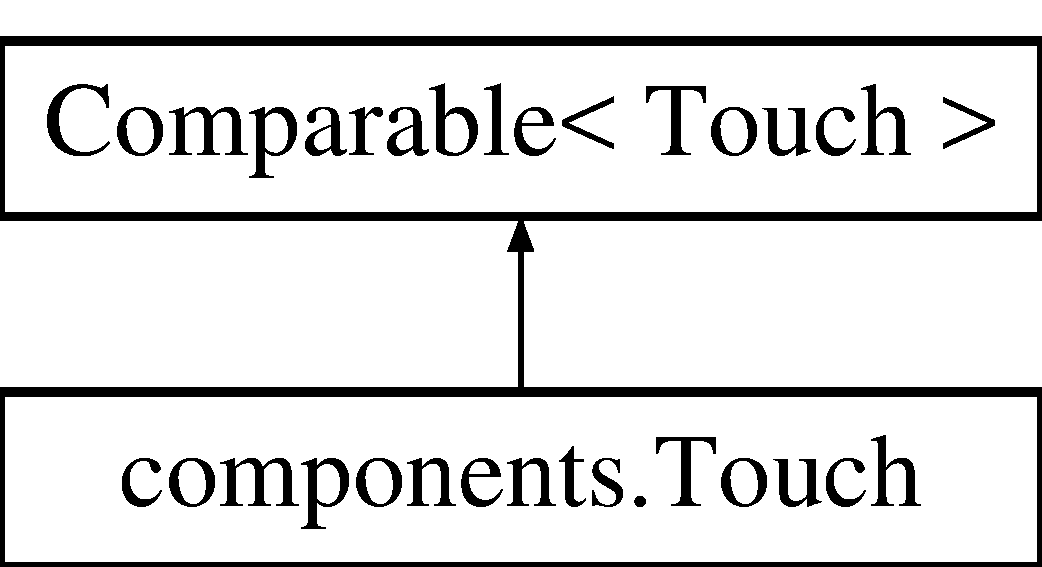
\includegraphics[height=2.000000cm]{classcomponents_1_1_touch}
\end{center}
\end{figure}
\subsection*{Public Member Functions}
\begin{DoxyCompactItemize}
\item 
\hyperlink{classcomponents_1_1_touch_abb291d0bd5aa18b2fbec3bf1d0d3f3fa}{Touch} (int keycode, double pressure, long timestamp)
\item 
\hyperlink{classcomponents_1_1_touch_a371ee9fd78523d19ee3b3ab9b57f5aff}{Touch} (\hyperlink{classcomponents_1_1_touch}{Touch} t)
\begin{DoxyCompactList}\small\item\em copy constructor \end{DoxyCompactList}\item 
void \hyperlink{classcomponents_1_1_touch_a407c6a87b0109d73ac0c84c32a38caf4}{set\+\_\+probability} (\hyperlink{classcomponents_1_1_window}{Window} preceeding\+\_\+window, double p)
\begin{DoxyCompactList}\small\item\em sets the probability that this touch succeeds a given sequence. Reccord the sequence and the probability \end{DoxyCompactList}\item 
double \hyperlink{classcomponents_1_1_touch_aa7eaadaf00950e7e7076136be30d00bd}{get\+\_\+probability} (\hyperlink{classcomponents_1_1_window}{Window} preceeding\+\_\+window)
\begin{DoxyCompactList}\small\item\em returns the probability of the touch occurring after a given window w. If the window does not exist return (T\+O\+DO) currently returning 0 \end{DoxyCompactList}\item 
double \hyperlink{classcomponents_1_1_touch_aa47273ddf1ef9ed00285bcee6cfd4eba}{get\+\_\+pressure} ()
\item 
int \hyperlink{classcomponents_1_1_touch_a7c61094e11f0dfeaf37e72a67fd04121}{get\+\_\+key} ()
\item 
long \hyperlink{classcomponents_1_1_touch_aab5b8034bd2970c1d7a2169adfcf53e6}{get\+\_\+timestamp} ()
\item 
boolean \hyperlink{classcomponents_1_1_touch_a7cb910d6f460cc8ba5f101786131e07d}{compare\+\_\+with\+\_\+token} (List$<$ \hyperlink{classcomponents_1_1_token}{Token} $>$ tokens, \hyperlink{classcomponents_1_1_touch}{Touch} other\+\_\+touch)
\item 
int \hyperlink{classcomponents_1_1_touch_ad38a5ddb406184988bcbcef0cfdad373}{hash\+Code} ()
\begin{DoxyCompactList}\small\item\em implement hash function for the touch class \end{DoxyCompactList}\item 
int \hyperlink{classcomponents_1_1_touch_a2dccbff3f4d150931886920d98354a17}{compare\+To} (\hyperlink{classcomponents_1_1_touch}{Touch} other\+\_\+touch)
\begin{DoxyCompactList}\small\item\em compare touches to one another. return negative if this touch is less than other\+\_\+touch \end{DoxyCompactList}\item 
String \hyperlink{classcomponents_1_1_touch_a6057203674219c31ed9c8c61e65a5686}{to\+String} ()
\end{DoxyCompactItemize}


\subsection{Detailed Description}
This class represents a touch event. 

\subsection{Constructor \& Destructor Documentation}
\index{components\+::\+Touch@{components\+::\+Touch}!Touch@{Touch}}
\index{Touch@{Touch}!components\+::\+Touch@{components\+::\+Touch}}
\subsubsection[{\texorpdfstring{Touch(int keycode, double pressure, long timestamp)}{Touch(int keycode, double pressure, long timestamp)}}]{\setlength{\rightskip}{0pt plus 5cm}components.\+Touch.\+Touch (
\begin{DoxyParamCaption}
\item[{int}]{keycode, }
\item[{double}]{pressure, }
\item[{long}]{timestamp}
\end{DoxyParamCaption}
)}\hypertarget{classcomponents_1_1_touch_abb291d0bd5aa18b2fbec3bf1d0d3f3fa}{}\label{classcomponents_1_1_touch_abb291d0bd5aa18b2fbec3bf1d0d3f3fa}
\index{components\+::\+Touch@{components\+::\+Touch}!Touch@{Touch}}
\index{Touch@{Touch}!components\+::\+Touch@{components\+::\+Touch}}
\subsubsection[{\texorpdfstring{Touch(\+Touch t)}{Touch(Touch t)}}]{\setlength{\rightskip}{0pt plus 5cm}components.\+Touch.\+Touch (
\begin{DoxyParamCaption}
\item[{{\bf Touch}}]{t}
\end{DoxyParamCaption}
)}\hypertarget{classcomponents_1_1_touch_a371ee9fd78523d19ee3b3ab9b57f5aff}{}\label{classcomponents_1_1_touch_a371ee9fd78523d19ee3b3ab9b57f5aff}


copy constructor 



\subsection{Member Function Documentation}
\index{components\+::\+Touch@{components\+::\+Touch}!compare\+\_\+with\+\_\+token@{compare\+\_\+with\+\_\+token}}
\index{compare\+\_\+with\+\_\+token@{compare\+\_\+with\+\_\+token}!components\+::\+Touch@{components\+::\+Touch}}
\subsubsection[{\texorpdfstring{compare\+\_\+with\+\_\+token(\+List$<$ Token $>$ tokens, Touch other\+\_\+touch)}{compare_with_token(List< Token > tokens, Touch other_touch)}}]{\setlength{\rightskip}{0pt plus 5cm}boolean components.\+Touch.\+compare\+\_\+with\+\_\+token (
\begin{DoxyParamCaption}
\item[{List$<$ {\bf Token} $>$}]{tokens, }
\item[{{\bf Touch}}]{other\+\_\+touch}
\end{DoxyParamCaption}
)}\hypertarget{classcomponents_1_1_touch_a7cb910d6f460cc8ba5f101786131e07d}{}\label{classcomponents_1_1_touch_a7cb910d6f460cc8ba5f101786131e07d}
compares the touches with the given token list. this function will return true if the touches are contained within the smae token \index{components\+::\+Touch@{components\+::\+Touch}!compare\+To@{compare\+To}}
\index{compare\+To@{compare\+To}!components\+::\+Touch@{components\+::\+Touch}}
\subsubsection[{\texorpdfstring{compare\+To(\+Touch other\+\_\+touch)}{compareTo(Touch other_touch)}}]{\setlength{\rightskip}{0pt plus 5cm}int components.\+Touch.\+compare\+To (
\begin{DoxyParamCaption}
\item[{{\bf Touch}}]{other\+\_\+touch}
\end{DoxyParamCaption}
)}\hypertarget{classcomponents_1_1_touch_a2dccbff3f4d150931886920d98354a17}{}\label{classcomponents_1_1_touch_a2dccbff3f4d150931886920d98354a17}


compare touches to one another. return negative if this touch is less than other\+\_\+touch 

\index{components\+::\+Touch@{components\+::\+Touch}!get\+\_\+key@{get\+\_\+key}}
\index{get\+\_\+key@{get\+\_\+key}!components\+::\+Touch@{components\+::\+Touch}}
\subsubsection[{\texorpdfstring{get\+\_\+key()}{get_key()}}]{\setlength{\rightskip}{0pt plus 5cm}int components.\+Touch.\+get\+\_\+key (
\begin{DoxyParamCaption}
{}
\end{DoxyParamCaption}
)}\hypertarget{classcomponents_1_1_touch_a7c61094e11f0dfeaf37e72a67fd04121}{}\label{classcomponents_1_1_touch_a7c61094e11f0dfeaf37e72a67fd04121}
\index{components\+::\+Touch@{components\+::\+Touch}!get\+\_\+pressure@{get\+\_\+pressure}}
\index{get\+\_\+pressure@{get\+\_\+pressure}!components\+::\+Touch@{components\+::\+Touch}}
\subsubsection[{\texorpdfstring{get\+\_\+pressure()}{get_pressure()}}]{\setlength{\rightskip}{0pt plus 5cm}double components.\+Touch.\+get\+\_\+pressure (
\begin{DoxyParamCaption}
{}
\end{DoxyParamCaption}
)}\hypertarget{classcomponents_1_1_touch_aa47273ddf1ef9ed00285bcee6cfd4eba}{}\label{classcomponents_1_1_touch_aa47273ddf1ef9ed00285bcee6cfd4eba}
\index{components\+::\+Touch@{components\+::\+Touch}!get\+\_\+probability@{get\+\_\+probability}}
\index{get\+\_\+probability@{get\+\_\+probability}!components\+::\+Touch@{components\+::\+Touch}}
\subsubsection[{\texorpdfstring{get\+\_\+probability(\+Window preceeding\+\_\+window)}{get_probability(Window preceeding_window)}}]{\setlength{\rightskip}{0pt plus 5cm}double components.\+Touch.\+get\+\_\+probability (
\begin{DoxyParamCaption}
\item[{{\bf Window}}]{preceeding\+\_\+window}
\end{DoxyParamCaption}
)}\hypertarget{classcomponents_1_1_touch_aa7eaadaf00950e7e7076136be30d00bd}{}\label{classcomponents_1_1_touch_aa7eaadaf00950e7e7076136be30d00bd}


returns the probability of the touch occurring after a given window w. If the window does not exist return (T\+O\+DO) currently returning 0 

\index{components\+::\+Touch@{components\+::\+Touch}!get\+\_\+timestamp@{get\+\_\+timestamp}}
\index{get\+\_\+timestamp@{get\+\_\+timestamp}!components\+::\+Touch@{components\+::\+Touch}}
\subsubsection[{\texorpdfstring{get\+\_\+timestamp()}{get_timestamp()}}]{\setlength{\rightskip}{0pt plus 5cm}long components.\+Touch.\+get\+\_\+timestamp (
\begin{DoxyParamCaption}
{}
\end{DoxyParamCaption}
)}\hypertarget{classcomponents_1_1_touch_aab5b8034bd2970c1d7a2169adfcf53e6}{}\label{classcomponents_1_1_touch_aab5b8034bd2970c1d7a2169adfcf53e6}
\index{components\+::\+Touch@{components\+::\+Touch}!hash\+Code@{hash\+Code}}
\index{hash\+Code@{hash\+Code}!components\+::\+Touch@{components\+::\+Touch}}
\subsubsection[{\texorpdfstring{hash\+Code()}{hashCode()}}]{\setlength{\rightskip}{0pt plus 5cm}int components.\+Touch.\+hash\+Code (
\begin{DoxyParamCaption}
{}
\end{DoxyParamCaption}
)}\hypertarget{classcomponents_1_1_touch_ad38a5ddb406184988bcbcef0cfdad373}{}\label{classcomponents_1_1_touch_ad38a5ddb406184988bcbcef0cfdad373}


implement hash function for the touch class 

\index{components\+::\+Touch@{components\+::\+Touch}!set\+\_\+probability@{set\+\_\+probability}}
\index{set\+\_\+probability@{set\+\_\+probability}!components\+::\+Touch@{components\+::\+Touch}}
\subsubsection[{\texorpdfstring{set\+\_\+probability(\+Window preceeding\+\_\+window, double p)}{set_probability(Window preceeding_window, double p)}}]{\setlength{\rightskip}{0pt plus 5cm}void components.\+Touch.\+set\+\_\+probability (
\begin{DoxyParamCaption}
\item[{{\bf Window}}]{preceeding\+\_\+window, }
\item[{double}]{p}
\end{DoxyParamCaption}
)}\hypertarget{classcomponents_1_1_touch_a407c6a87b0109d73ac0c84c32a38caf4}{}\label{classcomponents_1_1_touch_a407c6a87b0109d73ac0c84c32a38caf4}


sets the probability that this touch succeeds a given sequence. Reccord the sequence and the probability 

\index{components\+::\+Touch@{components\+::\+Touch}!to\+String@{to\+String}}
\index{to\+String@{to\+String}!components\+::\+Touch@{components\+::\+Touch}}
\subsubsection[{\texorpdfstring{to\+String()}{toString()}}]{\setlength{\rightskip}{0pt plus 5cm}String components.\+Touch.\+to\+String (
\begin{DoxyParamCaption}
{}
\end{DoxyParamCaption}
)}\hypertarget{classcomponents_1_1_touch_a6057203674219c31ed9c8c61e65a5686}{}\label{classcomponents_1_1_touch_a6057203674219c31ed9c8c61e65a5686}


The documentation for this class was generated from the following file\+:\begin{DoxyCompactItemize}
\item 
/home/element/\+P\+U\+F/\+Keyboard/java\+\_\+scripts/java\+\_\+marcov\+\_\+model/src/components/\hyperlink{_touch_8java}{Touch.\+java}\end{DoxyCompactItemize}

\hypertarget{classtrie_1_1_trie}{}\section{trie.\+Trie Class Reference}
\label{classtrie_1_1_trie}\index{trie.\+Trie@{trie.\+Trie}}


Implementation of Prefix Tree.  


\subsection*{Classes}
\begin{DoxyCompactItemize}
\item 
class {\bfseries Trie\+Node}
\end{DoxyCompactItemize}
\subsection*{Public Member Functions}
\begin{DoxyCompactItemize}
\item 
\hyperlink{classtrie_1_1_trie_a73835e6c18e8a44616d8995fd8f8a359}{Trie} ()
\begin{DoxyCompactList}\small\item\em sets up the tree so that everything will be added to trienode root? \end{DoxyCompactList}\item 
\hyperlink{classtrie_1_1_trie_abcb888636eae05bbb59fb418fcf46732}{Trie} (\hyperlink{classtrie_1_1_trie}{Trie} t)
\begin{DoxyCompactList}\small\item\em creates a copy trie \end{DoxyCompactList}\item 
void \hyperlink{classtrie_1_1_trie_aeca1e283716cb4db6e52907049d08acb}{clear} ()
\begin{DoxyCompactList}\small\item\em removes all elements from the trie \end{DoxyCompactList}\item 
void \hyperlink{classtrie_1_1_trie_afc2ab785d2546e95b2698c46f76d9c77}{insert\+String} (String s, int index)
\item 
int \hyperlink{classtrie_1_1_trie_a061c92ea6abc9e1d9e6e6ac5c0c0b4b2}{occurrence\+\_\+count} (String s)
\begin{DoxyCompactList}\small\item\em retrieves the number of occurrences of a given string in the tree \end{DoxyCompactList}\item 
List$<$ Integer $>$ \hyperlink{classtrie_1_1_trie_a0755a2fdc3ebc07406db5a5ff1310f38}{get\+\_\+index\+\_\+list} (String s)
\begin{DoxyCompactList}\small\item\em returns a list of indexes containing the given window \end{DoxyCompactList}\item 
void \hyperlink{classtrie_1_1_trie_a3faeec11a80f63081cde7973fe32be50}{print\+Sorted} (Trie\+Node node, String s)
\begin{DoxyCompactList}\small\item\em prints the elements in a sorted order \end{DoxyCompactList}\end{DoxyCompactItemize}


\subsection{Detailed Description}
Implementation of Prefix Tree. 

This benefits the efficiency of the program. This class is used primarily to figure out information about windows needed in the probability computation. 

\subsection{Constructor \& Destructor Documentation}
\index{trie\+::\+Trie@{trie\+::\+Trie}!Trie@{Trie}}
\index{Trie@{Trie}!trie\+::\+Trie@{trie\+::\+Trie}}
\subsubsection[{\texorpdfstring{Trie()}{Trie()}}]{\setlength{\rightskip}{0pt plus 5cm}trie.\+Trie.\+Trie (
\begin{DoxyParamCaption}
{}
\end{DoxyParamCaption}
)}\hypertarget{classtrie_1_1_trie_a73835e6c18e8a44616d8995fd8f8a359}{}\label{classtrie_1_1_trie_a73835e6c18e8a44616d8995fd8f8a359}


sets up the tree so that everything will be added to trienode root? 

\index{trie\+::\+Trie@{trie\+::\+Trie}!Trie@{Trie}}
\index{Trie@{Trie}!trie\+::\+Trie@{trie\+::\+Trie}}
\subsubsection[{\texorpdfstring{Trie(\+Trie t)}{Trie(Trie t)}}]{\setlength{\rightskip}{0pt plus 5cm}trie.\+Trie.\+Trie (
\begin{DoxyParamCaption}
\item[{{\bf Trie}}]{t}
\end{DoxyParamCaption}
)}\hypertarget{classtrie_1_1_trie_abcb888636eae05bbb59fb418fcf46732}{}\label{classtrie_1_1_trie_abcb888636eae05bbb59fb418fcf46732}


creates a copy trie 



\subsection{Member Function Documentation}
\index{trie\+::\+Trie@{trie\+::\+Trie}!clear@{clear}}
\index{clear@{clear}!trie\+::\+Trie@{trie\+::\+Trie}}
\subsubsection[{\texorpdfstring{clear()}{clear()}}]{\setlength{\rightskip}{0pt plus 5cm}void trie.\+Trie.\+clear (
\begin{DoxyParamCaption}
{}
\end{DoxyParamCaption}
)}\hypertarget{classtrie_1_1_trie_aeca1e283716cb4db6e52907049d08acb}{}\label{classtrie_1_1_trie_aeca1e283716cb4db6e52907049d08acb}


removes all elements from the trie 



Here is the caller graph for this function\+:\nopagebreak
\begin{figure}[H]
\begin{center}
\leavevmode
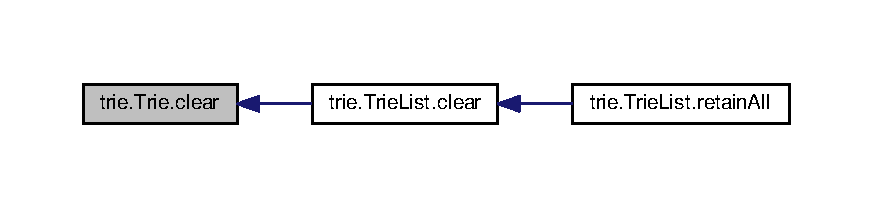
\includegraphics[width=350pt]{classtrie_1_1_trie_aeca1e283716cb4db6e52907049d08acb_icgraph}
\end{center}
\end{figure}


\index{trie\+::\+Trie@{trie\+::\+Trie}!get\+\_\+index\+\_\+list@{get\+\_\+index\+\_\+list}}
\index{get\+\_\+index\+\_\+list@{get\+\_\+index\+\_\+list}!trie\+::\+Trie@{trie\+::\+Trie}}
\subsubsection[{\texorpdfstring{get\+\_\+index\+\_\+list(\+String s)}{get_index_list(String s)}}]{\setlength{\rightskip}{0pt plus 5cm}List$<$Integer$>$ trie.\+Trie.\+get\+\_\+index\+\_\+list (
\begin{DoxyParamCaption}
\item[{String}]{s}
\end{DoxyParamCaption}
)}\hypertarget{classtrie_1_1_trie_a0755a2fdc3ebc07406db5a5ff1310f38}{}\label{classtrie_1_1_trie_a0755a2fdc3ebc07406db5a5ff1310f38}


returns a list of indexes containing the given window 



Here is the caller graph for this function\+:\nopagebreak
\begin{figure}[H]
\begin{center}
\leavevmode
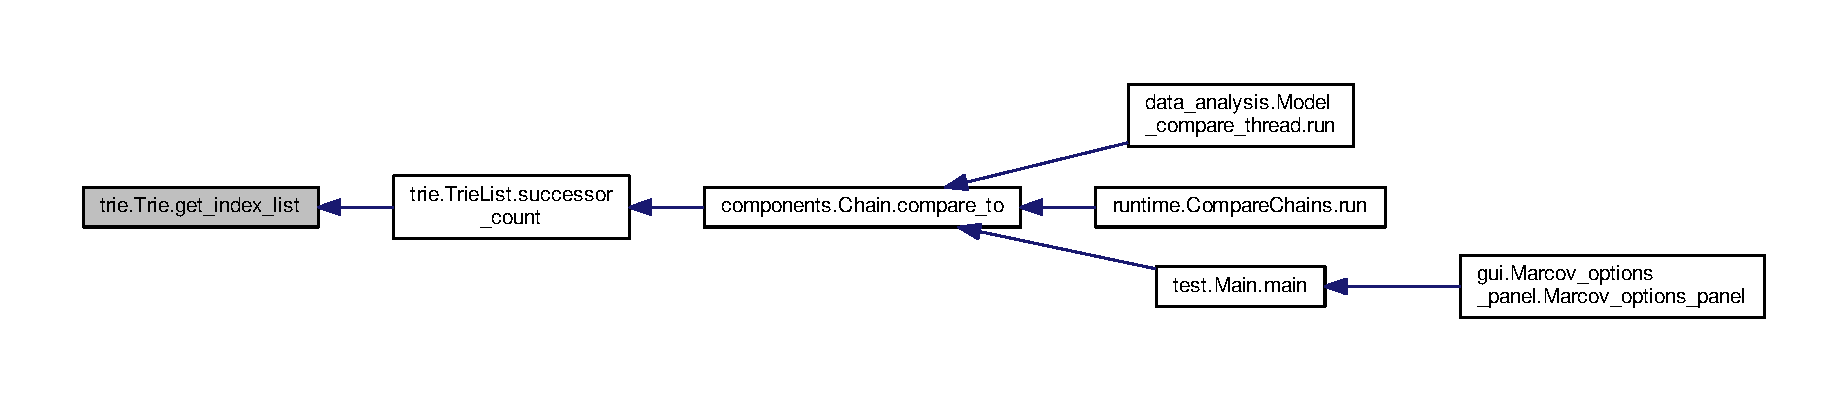
\includegraphics[width=350pt]{classtrie_1_1_trie_a0755a2fdc3ebc07406db5a5ff1310f38_icgraph}
\end{center}
\end{figure}


\index{trie\+::\+Trie@{trie\+::\+Trie}!insert\+String@{insert\+String}}
\index{insert\+String@{insert\+String}!trie\+::\+Trie@{trie\+::\+Trie}}
\subsubsection[{\texorpdfstring{insert\+String(\+String s, int index)}{insertString(String s, int index)}}]{\setlength{\rightskip}{0pt plus 5cm}void trie.\+Trie.\+insert\+String (
\begin{DoxyParamCaption}
\item[{String}]{s, }
\item[{int}]{index}
\end{DoxyParamCaption}
)}\hypertarget{classtrie_1_1_trie_afc2ab785d2546e95b2698c46f76d9c77}{}\label{classtrie_1_1_trie_afc2ab785d2546e95b2698c46f76d9c77}


Here is the caller graph for this function\+:\nopagebreak
\begin{figure}[H]
\begin{center}
\leavevmode
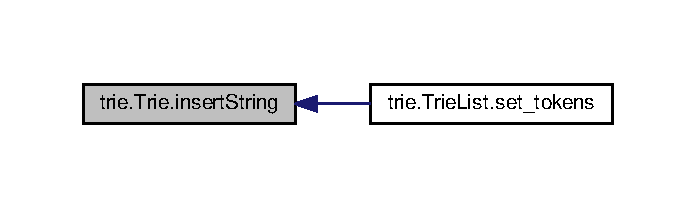
\includegraphics[width=334pt]{classtrie_1_1_trie_afc2ab785d2546e95b2698c46f76d9c77_icgraph}
\end{center}
\end{figure}


\index{trie\+::\+Trie@{trie\+::\+Trie}!occurrence\+\_\+count@{occurrence\+\_\+count}}
\index{occurrence\+\_\+count@{occurrence\+\_\+count}!trie\+::\+Trie@{trie\+::\+Trie}}
\subsubsection[{\texorpdfstring{occurrence\+\_\+count(\+String s)}{occurrence_count(String s)}}]{\setlength{\rightskip}{0pt plus 5cm}int trie.\+Trie.\+occurrence\+\_\+count (
\begin{DoxyParamCaption}
\item[{String}]{s}
\end{DoxyParamCaption}
)}\hypertarget{classtrie_1_1_trie_a061c92ea6abc9e1d9e6e6ac5c0c0b4b2}{}\label{classtrie_1_1_trie_a061c92ea6abc9e1d9e6e6ac5c0c0b4b2}


retrieves the number of occurrences of a given string in the tree 



Here is the caller graph for this function\+:\nopagebreak
\begin{figure}[H]
\begin{center}
\leavevmode
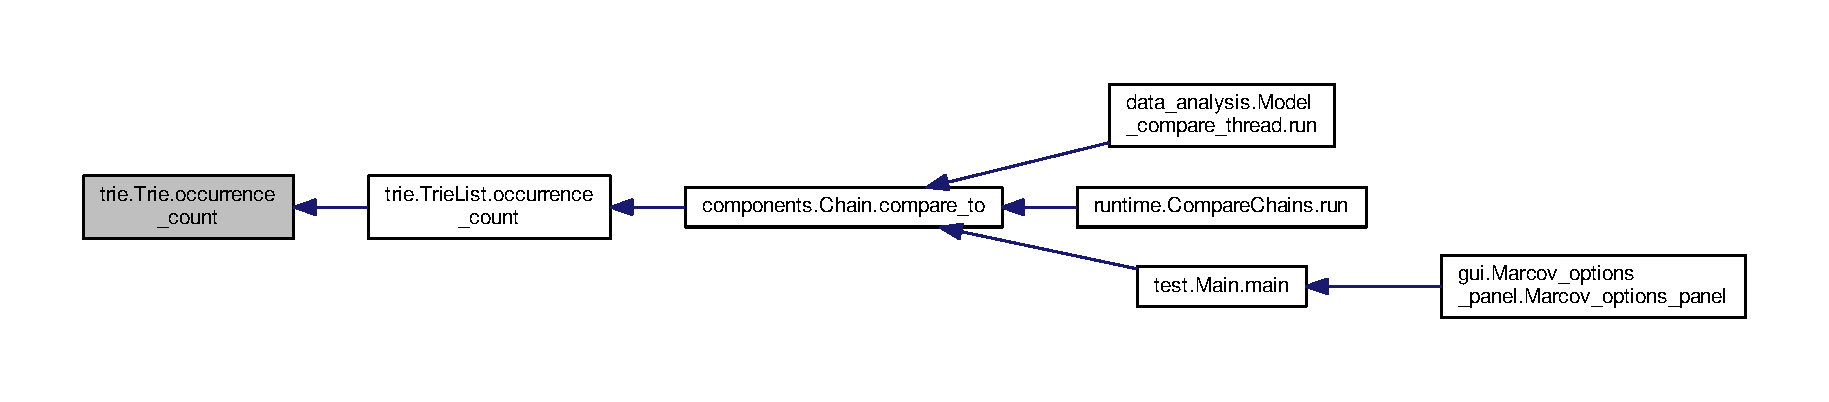
\includegraphics[width=350pt]{classtrie_1_1_trie_a061c92ea6abc9e1d9e6e6ac5c0c0b4b2_icgraph}
\end{center}
\end{figure}


\index{trie\+::\+Trie@{trie\+::\+Trie}!print\+Sorted@{print\+Sorted}}
\index{print\+Sorted@{print\+Sorted}!trie\+::\+Trie@{trie\+::\+Trie}}
\subsubsection[{\texorpdfstring{print\+Sorted(\+Trie\+Node node, String s)}{printSorted(TrieNode node, String s)}}]{\setlength{\rightskip}{0pt plus 5cm}void trie.\+Trie.\+print\+Sorted (
\begin{DoxyParamCaption}
\item[{Trie\+Node}]{node, }
\item[{String}]{s}
\end{DoxyParamCaption}
)}\hypertarget{classtrie_1_1_trie_a3faeec11a80f63081cde7973fe32be50}{}\label{classtrie_1_1_trie_a3faeec11a80f63081cde7973fe32be50}


prints the elements in a sorted order 



The documentation for this class was generated from the following file\+:\begin{DoxyCompactItemize}
\item 
/home/element/\+P\+U\+F/\+Keyboard/java\+\_\+scripts/java\+\_\+marcov\+\_\+model/src/trie/\hyperlink{_trie_8java}{Trie.\+java}\end{DoxyCompactItemize}

\hypertarget{classtrie_1_1_trie_list}{}\section{trie.\+Trie\+List Class Reference}
\label{classtrie_1_1_trie_list}\index{trie.\+Trie\+List@{trie.\+Trie\+List}}
Inheritance diagram for trie.\+Trie\+List\+:\begin{figure}[H]
\begin{center}
\leavevmode
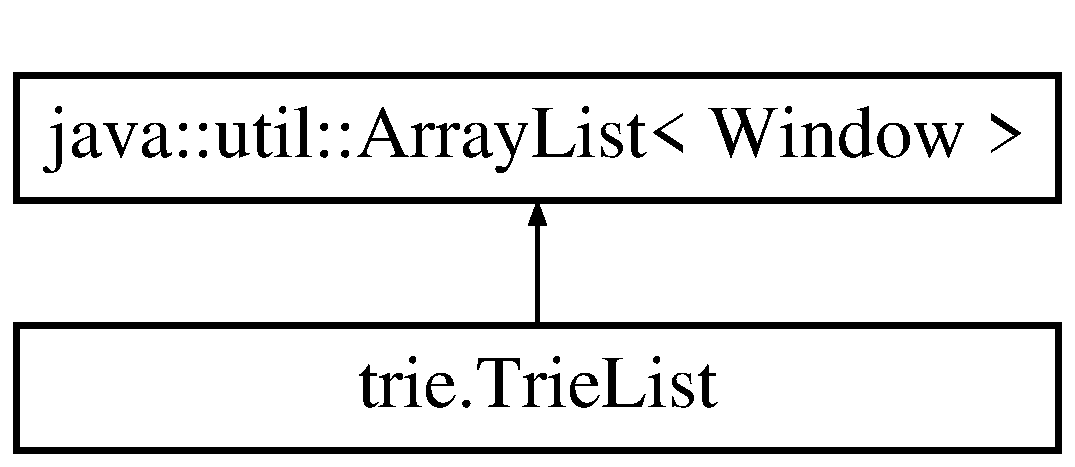
\includegraphics[height=2.000000cm]{classtrie_1_1_trie_list}
\end{center}
\end{figure}
\subsection*{Public Member Functions}
\begin{DoxyCompactItemize}
\item 
\hyperlink{classtrie_1_1_trie_list_a080afd57ffa7220ba51a4f8e8f16c7b4}{Trie\+List} ()
\item 
\hyperlink{classtrie_1_1_trie_list_a4edc08953617846d3d13050951a319e5}{Trie\+List} (\hyperlink{classtrie_1_1_trie_list}{Trie\+List} t)
\item 
boolean \hyperlink{classtrie_1_1_trie_list_a4b3c20b9e91337a4bbf3604fe2c66b3b}{add} (\hyperlink{classcomponents_1_1_window}{Window} arg0)
\item 
void \hyperlink{classtrie_1_1_trie_list_a857adbaf3b3c81d7bacf6b8258920a0c}{add} (int arg0, \hyperlink{classcomponents_1_1_window}{Window} arg1)
\item 
boolean \hyperlink{classtrie_1_1_trie_list_a51ba821144816982deb88f4c25ab4966}{add\+All} (Collection$<$?extends \hyperlink{classcomponents_1_1_window}{Window} $>$ arg0)
\item 
boolean \hyperlink{classtrie_1_1_trie_list_a522999ec5023a861fa914af49bcde0d2}{add\+All} (int arg0, Collection$<$?extends \hyperlink{classcomponents_1_1_window}{Window} $>$ arg1)
\item 
void \hyperlink{classtrie_1_1_trie_list_a6bfa2ade95d246ea95a3071993f1600f}{clear} ()
\item 
boolean \hyperlink{classtrie_1_1_trie_list_a5b290c36befb18333f000caf4c0080e1}{remove} (Object arg0)
\item 
\hyperlink{classcomponents_1_1_window}{Window} \hyperlink{classtrie_1_1_trie_list_ac4e6c299679bd53f8f38f87dac12bdb0}{remove} (int arg0)
\item 
boolean \hyperlink{classtrie_1_1_trie_list_ae0298e14b450853968bc61a88fb41dfe}{remove\+All} (Collection$<$?$>$ arg0)
\item 
boolean \hyperlink{classtrie_1_1_trie_list_a49157c8085a17723c493b3cf1fe112e6}{retain\+All} (Collection$<$?$>$ arg0)
\item 
\hyperlink{classcomponents_1_1_window}{Window} \hyperlink{classtrie_1_1_trie_list_aa23a0325d6d9ccd4fda580073cf40954}{set} (int arg0, \hyperlink{classcomponents_1_1_window}{Window} arg1)
\item 
int \hyperlink{classtrie_1_1_trie_list_a42644a837b91c05c2db9a106bd02e30d}{successor\+\_\+count} (List$<$ \hyperlink{classcomponents_1_1_touch}{Touch} $>$ successor\+\_\+list, \hyperlink{classcomponents_1_1_window}{Window} window, \hyperlink{classcomponents_1_1_touch}{Touch} touch)
\begin{DoxyCompactList}\small\item\em counts the number of times a given touch comes after a given window. in the given window, succesors list \end{DoxyCompactList}\item 
int \hyperlink{classtrie_1_1_trie_list_a3748bb1aaf4f32d26b74091eb3b3706d}{occurrence\+\_\+count} (\hyperlink{classcomponents_1_1_window}{Window} w)
\item 
void \hyperlink{classtrie_1_1_trie_list_a5e339d095e6b1d843f34ec3091612c4e}{set\+\_\+tokens} (List$<$ \hyperlink{classcomponents_1_1_token}{Token} $>$ tokens)
\begin{DoxyCompactList}\small\item\em sets the tokens that will be used when encoding the window \end{DoxyCompactList}\end{DoxyCompactItemize}


\subsection{Detailed Description}
T\+O\+DO Eventually this will be implemented as a prefix tree. This will greatly speed up many of the operations causing the calculation of the probabilities to be slow. right now it is fine to have the backing be an arraylist overrided methods are any that remove, modify, or add to the arraylist. these methods will also change the prefix tree 

\subsection{Constructor \& Destructor Documentation}
\index{trie\+::\+Trie\+List@{trie\+::\+Trie\+List}!Trie\+List@{Trie\+List}}
\index{Trie\+List@{Trie\+List}!trie\+::\+Trie\+List@{trie\+::\+Trie\+List}}
\subsubsection[{\texorpdfstring{Trie\+List()}{TrieList()}}]{\setlength{\rightskip}{0pt plus 5cm}trie.\+Trie\+List.\+Trie\+List (
\begin{DoxyParamCaption}
{}
\end{DoxyParamCaption}
)}\hypertarget{classtrie_1_1_trie_list_a080afd57ffa7220ba51a4f8e8f16c7b4}{}\label{classtrie_1_1_trie_list_a080afd57ffa7220ba51a4f8e8f16c7b4}
\index{trie\+::\+Trie\+List@{trie\+::\+Trie\+List}!Trie\+List@{Trie\+List}}
\index{Trie\+List@{Trie\+List}!trie\+::\+Trie\+List@{trie\+::\+Trie\+List}}
\subsubsection[{\texorpdfstring{Trie\+List(\+Trie\+List t)}{TrieList(TrieList t)}}]{\setlength{\rightskip}{0pt plus 5cm}trie.\+Trie\+List.\+Trie\+List (
\begin{DoxyParamCaption}
\item[{{\bf Trie\+List}}]{t}
\end{DoxyParamCaption}
)}\hypertarget{classtrie_1_1_trie_list_a4edc08953617846d3d13050951a319e5}{}\label{classtrie_1_1_trie_list_a4edc08953617846d3d13050951a319e5}


\subsection{Member Function Documentation}
\index{trie\+::\+Trie\+List@{trie\+::\+Trie\+List}!add@{add}}
\index{add@{add}!trie\+::\+Trie\+List@{trie\+::\+Trie\+List}}
\subsubsection[{\texorpdfstring{add(\+Window arg0)}{add(Window arg0)}}]{\setlength{\rightskip}{0pt plus 5cm}boolean trie.\+Trie\+List.\+add (
\begin{DoxyParamCaption}
\item[{{\bf Window}}]{arg0}
\end{DoxyParamCaption}
)}\hypertarget{classtrie_1_1_trie_list_a4b3c20b9e91337a4bbf3604fe2c66b3b}{}\label{classtrie_1_1_trie_list_a4b3c20b9e91337a4bbf3604fe2c66b3b}
\index{trie\+::\+Trie\+List@{trie\+::\+Trie\+List}!add@{add}}
\index{add@{add}!trie\+::\+Trie\+List@{trie\+::\+Trie\+List}}
\subsubsection[{\texorpdfstring{add(int arg0, Window arg1)}{add(int arg0, Window arg1)}}]{\setlength{\rightskip}{0pt plus 5cm}void trie.\+Trie\+List.\+add (
\begin{DoxyParamCaption}
\item[{int}]{arg0, }
\item[{{\bf Window}}]{arg1}
\end{DoxyParamCaption}
)}\hypertarget{classtrie_1_1_trie_list_a857adbaf3b3c81d7bacf6b8258920a0c}{}\label{classtrie_1_1_trie_list_a857adbaf3b3c81d7bacf6b8258920a0c}
\index{trie\+::\+Trie\+List@{trie\+::\+Trie\+List}!add\+All@{add\+All}}
\index{add\+All@{add\+All}!trie\+::\+Trie\+List@{trie\+::\+Trie\+List}}
\subsubsection[{\texorpdfstring{add\+All(\+Collection$<$?extends Window $>$ arg0)}{addAll(Collection<?extends Window > arg0)}}]{\setlength{\rightskip}{0pt plus 5cm}boolean trie.\+Trie\+List.\+add\+All (
\begin{DoxyParamCaption}
\item[{Collection$<$?extends {\bf Window} $>$}]{arg0}
\end{DoxyParamCaption}
)}\hypertarget{classtrie_1_1_trie_list_a51ba821144816982deb88f4c25ab4966}{}\label{classtrie_1_1_trie_list_a51ba821144816982deb88f4c25ab4966}
\index{trie\+::\+Trie\+List@{trie\+::\+Trie\+List}!add\+All@{add\+All}}
\index{add\+All@{add\+All}!trie\+::\+Trie\+List@{trie\+::\+Trie\+List}}
\subsubsection[{\texorpdfstring{add\+All(int arg0, Collection$<$?extends Window $>$ arg1)}{addAll(int arg0, Collection<?extends Window > arg1)}}]{\setlength{\rightskip}{0pt plus 5cm}boolean trie.\+Trie\+List.\+add\+All (
\begin{DoxyParamCaption}
\item[{int}]{arg0, }
\item[{Collection$<$?extends {\bf Window} $>$}]{arg1}
\end{DoxyParamCaption}
)}\hypertarget{classtrie_1_1_trie_list_a522999ec5023a861fa914af49bcde0d2}{}\label{classtrie_1_1_trie_list_a522999ec5023a861fa914af49bcde0d2}
\index{trie\+::\+Trie\+List@{trie\+::\+Trie\+List}!clear@{clear}}
\index{clear@{clear}!trie\+::\+Trie\+List@{trie\+::\+Trie\+List}}
\subsubsection[{\texorpdfstring{clear()}{clear()}}]{\setlength{\rightskip}{0pt plus 5cm}void trie.\+Trie\+List.\+clear (
\begin{DoxyParamCaption}
{}
\end{DoxyParamCaption}
)}\hypertarget{classtrie_1_1_trie_list_a6bfa2ade95d246ea95a3071993f1600f}{}\label{classtrie_1_1_trie_list_a6bfa2ade95d246ea95a3071993f1600f}
\index{trie\+::\+Trie\+List@{trie\+::\+Trie\+List}!occurrence\+\_\+count@{occurrence\+\_\+count}}
\index{occurrence\+\_\+count@{occurrence\+\_\+count}!trie\+::\+Trie\+List@{trie\+::\+Trie\+List}}
\subsubsection[{\texorpdfstring{occurrence\+\_\+count(\+Window w)}{occurrence_count(Window w)}}]{\setlength{\rightskip}{0pt plus 5cm}int trie.\+Trie\+List.\+occurrence\+\_\+count (
\begin{DoxyParamCaption}
\item[{{\bf Window}}]{w}
\end{DoxyParamCaption}
)}\hypertarget{classtrie_1_1_trie_list_a3748bb1aaf4f32d26b74091eb3b3706d}{}\label{classtrie_1_1_trie_list_a3748bb1aaf4f32d26b74091eb3b3706d}
return the number of occurrences of w in window\+\_\+list T\+O\+DO I think this method needs to be faster. Storing windows in a prefix tree would allow for this \index{trie\+::\+Trie\+List@{trie\+::\+Trie\+List}!remove@{remove}}
\index{remove@{remove}!trie\+::\+Trie\+List@{trie\+::\+Trie\+List}}
\subsubsection[{\texorpdfstring{remove(\+Object arg0)}{remove(Object arg0)}}]{\setlength{\rightskip}{0pt plus 5cm}boolean trie.\+Trie\+List.\+remove (
\begin{DoxyParamCaption}
\item[{Object}]{arg0}
\end{DoxyParamCaption}
)}\hypertarget{classtrie_1_1_trie_list_a5b290c36befb18333f000caf4c0080e1}{}\label{classtrie_1_1_trie_list_a5b290c36befb18333f000caf4c0080e1}
\index{trie\+::\+Trie\+List@{trie\+::\+Trie\+List}!remove@{remove}}
\index{remove@{remove}!trie\+::\+Trie\+List@{trie\+::\+Trie\+List}}
\subsubsection[{\texorpdfstring{remove(int arg0)}{remove(int arg0)}}]{\setlength{\rightskip}{0pt plus 5cm}{\bf Window} trie.\+Trie\+List.\+remove (
\begin{DoxyParamCaption}
\item[{int}]{arg0}
\end{DoxyParamCaption}
)}\hypertarget{classtrie_1_1_trie_list_ac4e6c299679bd53f8f38f87dac12bdb0}{}\label{classtrie_1_1_trie_list_ac4e6c299679bd53f8f38f87dac12bdb0}
\index{trie\+::\+Trie\+List@{trie\+::\+Trie\+List}!remove\+All@{remove\+All}}
\index{remove\+All@{remove\+All}!trie\+::\+Trie\+List@{trie\+::\+Trie\+List}}
\subsubsection[{\texorpdfstring{remove\+All(\+Collection$<$?$>$ arg0)}{removeAll(Collection<?> arg0)}}]{\setlength{\rightskip}{0pt plus 5cm}boolean trie.\+Trie\+List.\+remove\+All (
\begin{DoxyParamCaption}
\item[{Collection$<$?$>$}]{arg0}
\end{DoxyParamCaption}
)}\hypertarget{classtrie_1_1_trie_list_ae0298e14b450853968bc61a88fb41dfe}{}\label{classtrie_1_1_trie_list_ae0298e14b450853968bc61a88fb41dfe}
\index{trie\+::\+Trie\+List@{trie\+::\+Trie\+List}!retain\+All@{retain\+All}}
\index{retain\+All@{retain\+All}!trie\+::\+Trie\+List@{trie\+::\+Trie\+List}}
\subsubsection[{\texorpdfstring{retain\+All(\+Collection$<$?$>$ arg0)}{retainAll(Collection<?> arg0)}}]{\setlength{\rightskip}{0pt plus 5cm}boolean trie.\+Trie\+List.\+retain\+All (
\begin{DoxyParamCaption}
\item[{Collection$<$?$>$}]{arg0}
\end{DoxyParamCaption}
)}\hypertarget{classtrie_1_1_trie_list_a49157c8085a17723c493b3cf1fe112e6}{}\label{classtrie_1_1_trie_list_a49157c8085a17723c493b3cf1fe112e6}
\index{trie\+::\+Trie\+List@{trie\+::\+Trie\+List}!set@{set}}
\index{set@{set}!trie\+::\+Trie\+List@{trie\+::\+Trie\+List}}
\subsubsection[{\texorpdfstring{set(int arg0, Window arg1)}{set(int arg0, Window arg1)}}]{\setlength{\rightskip}{0pt plus 5cm}{\bf Window} trie.\+Trie\+List.\+set (
\begin{DoxyParamCaption}
\item[{int}]{arg0, }
\item[{{\bf Window}}]{arg1}
\end{DoxyParamCaption}
)}\hypertarget{classtrie_1_1_trie_list_aa23a0325d6d9ccd4fda580073cf40954}{}\label{classtrie_1_1_trie_list_aa23a0325d6d9ccd4fda580073cf40954}
\index{trie\+::\+Trie\+List@{trie\+::\+Trie\+List}!set\+\_\+tokens@{set\+\_\+tokens}}
\index{set\+\_\+tokens@{set\+\_\+tokens}!trie\+::\+Trie\+List@{trie\+::\+Trie\+List}}
\subsubsection[{\texorpdfstring{set\+\_\+tokens(\+List$<$ Token $>$ tokens)}{set_tokens(List< Token > tokens)}}]{\setlength{\rightskip}{0pt plus 5cm}void trie.\+Trie\+List.\+set\+\_\+tokens (
\begin{DoxyParamCaption}
\item[{List$<$ {\bf Token} $>$}]{tokens}
\end{DoxyParamCaption}
)}\hypertarget{classtrie_1_1_trie_list_a5e339d095e6b1d843f34ec3091612c4e}{}\label{classtrie_1_1_trie_list_a5e339d095e6b1d843f34ec3091612c4e}


sets the tokens that will be used when encoding the window 

\index{trie\+::\+Trie\+List@{trie\+::\+Trie\+List}!successor\+\_\+count@{successor\+\_\+count}}
\index{successor\+\_\+count@{successor\+\_\+count}!trie\+::\+Trie\+List@{trie\+::\+Trie\+List}}
\subsubsection[{\texorpdfstring{successor\+\_\+count(\+List$<$ Touch $>$ successor\+\_\+list, Window window, Touch touch)}{successor_count(List< Touch > successor_list, Window window, Touch touch)}}]{\setlength{\rightskip}{0pt plus 5cm}int trie.\+Trie\+List.\+successor\+\_\+count (
\begin{DoxyParamCaption}
\item[{List$<$ {\bf Touch} $>$}]{successor\+\_\+list, }
\item[{{\bf Window}}]{window, }
\item[{{\bf Touch}}]{touch}
\end{DoxyParamCaption}
)}\hypertarget{classtrie_1_1_trie_list_a42644a837b91c05c2db9a106bd02e30d}{}\label{classtrie_1_1_trie_list_a42644a837b91c05c2db9a106bd02e30d}


counts the number of times a given touch comes after a given window. in the given window, succesors list 



The documentation for this class was generated from the following file\+:\begin{DoxyCompactItemize}
\item 
/home/element/\+P\+U\+F/\+Keyboard/java\+\_\+scripts/java\+\_\+marcov\+\_\+model/src/trie/\hyperlink{_trie_list_8java}{Trie\+List.\+java}\end{DoxyCompactItemize}

\hypertarget{enumcomponents_1_1_token_1_1_type}{}\section{components.\+Token.\+Type Enum Reference}
\label{enumcomponents_1_1_token_1_1_type}\index{components.\+Token.\+Type@{components.\+Token.\+Type}}


specify the type of token we want to build  


\subsection*{Public Attributes}
\begin{DoxyCompactItemize}
\item 
\hyperlink{enumcomponents_1_1_token_1_1_type_ac32881b7c310d3276351f4209e598e3a}{linear}
\item 
\hyperlink{enumcomponents_1_1_token_1_1_type_a87c6d7380a042991b552b6b4fb33acdf}{keycode\+\_\+mu}
\item 
\hyperlink{enumcomponents_1_1_token_1_1_type_a7b9ca06099d60d90f8a502053a4aef4c}{combined}
\end{DoxyCompactItemize}


\subsection{Detailed Description}
specify the type of token we want to build 

\subsection{Member Data Documentation}
\index{components\+::\+Token\+::\+Type@{components\+::\+Token\+::\+Type}!combined@{combined}}
\index{combined@{combined}!components\+::\+Token\+::\+Type@{components\+::\+Token\+::\+Type}}
\subsubsection[{\texorpdfstring{combined}{combined}}]{\setlength{\rightskip}{0pt plus 5cm}components.\+Token.\+Type.\+combined}\hypertarget{enumcomponents_1_1_token_1_1_type_a7b9ca06099d60d90f8a502053a4aef4c}{}\label{enumcomponents_1_1_token_1_1_type_a7b9ca06099d60d90f8a502053a4aef4c}
\index{components\+::\+Token\+::\+Type@{components\+::\+Token\+::\+Type}!keycode\+\_\+mu@{keycode\+\_\+mu}}
\index{keycode\+\_\+mu@{keycode\+\_\+mu}!components\+::\+Token\+::\+Type@{components\+::\+Token\+::\+Type}}
\subsubsection[{\texorpdfstring{keycode\+\_\+mu}{keycode_mu}}]{\setlength{\rightskip}{0pt plus 5cm}components.\+Token.\+Type.\+keycode\+\_\+mu}\hypertarget{enumcomponents_1_1_token_1_1_type_a87c6d7380a042991b552b6b4fb33acdf}{}\label{enumcomponents_1_1_token_1_1_type_a87c6d7380a042991b552b6b4fb33acdf}
\index{components\+::\+Token\+::\+Type@{components\+::\+Token\+::\+Type}!linear@{linear}}
\index{linear@{linear}!components\+::\+Token\+::\+Type@{components\+::\+Token\+::\+Type}}
\subsubsection[{\texorpdfstring{linear}{linear}}]{\setlength{\rightskip}{0pt plus 5cm}components.\+Token.\+Type.\+linear}\hypertarget{enumcomponents_1_1_token_1_1_type_ac32881b7c310d3276351f4209e598e3a}{}\label{enumcomponents_1_1_token_1_1_type_ac32881b7c310d3276351f4209e598e3a}


The documentation for this enum was generated from the following file\+:\begin{DoxyCompactItemize}
\item 
/home/element/\+P\+U\+F/\+Keyboard/java\+\_\+scripts/java\+\_\+marcov\+\_\+model/src/components/\hyperlink{_token_8java}{Token.\+java}\end{DoxyCompactItemize}

\hypertarget{classjunit_1_1_unit___compare_chains_rank}{}\section{junit.\+Unit\+\_\+\+Compare\+Chains\+Rank Class Reference}
\label{classjunit_1_1_unit___compare_chains_rank}\index{junit.\+Unit\+\_\+\+Compare\+Chains\+Rank@{junit.\+Unit\+\_\+\+Compare\+Chains\+Rank}}


goal is to test compare chains rank functionality  


\subsection*{Public Member Functions}
\begin{DoxyCompactItemize}
\item 
void \hyperlink{classjunit_1_1_unit___compare_chains_rank_ade2cbca2acb0c46e78c006622cd2eec8}{init} ()
\item 
void \hyperlink{classjunit_1_1_unit___compare_chains_rank_adecfca92c2f0fb546dc44d77285d37d6}{test\+\_\+authentication\+\_\+probability} ()
\end{DoxyCompactItemize}


\subsection{Detailed Description}
goal is to test compare chains rank functionality 



\subsection{Member Function Documentation}
\index{junit\+::\+Unit\+\_\+\+Compare\+Chains\+Rank@{junit\+::\+Unit\+\_\+\+Compare\+Chains\+Rank}!init@{init}}
\index{init@{init}!junit\+::\+Unit\+\_\+\+Compare\+Chains\+Rank@{junit\+::\+Unit\+\_\+\+Compare\+Chains\+Rank}}
\subsubsection[{\texorpdfstring{init()}{init()}}]{\setlength{\rightskip}{0pt plus 5cm}void junit.\+Unit\+\_\+\+Compare\+Chains\+Rank.\+init (
\begin{DoxyParamCaption}
{}
\end{DoxyParamCaption}
)}\hypertarget{classjunit_1_1_unit___compare_chains_rank_ade2cbca2acb0c46e78c006622cd2eec8}{}\label{classjunit_1_1_unit___compare_chains_rank_ade2cbca2acb0c46e78c006622cd2eec8}


Here is the call graph for this function\+:\nopagebreak
\begin{figure}[H]
\begin{center}
\leavevmode
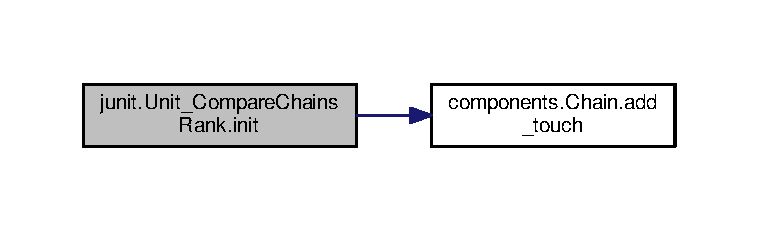
\includegraphics[width=350pt]{classjunit_1_1_unit___compare_chains_rank_ade2cbca2acb0c46e78c006622cd2eec8_cgraph}
\end{center}
\end{figure}


\index{junit\+::\+Unit\+\_\+\+Compare\+Chains\+Rank@{junit\+::\+Unit\+\_\+\+Compare\+Chains\+Rank}!test\+\_\+authentication\+\_\+probability@{test\+\_\+authentication\+\_\+probability}}
\index{test\+\_\+authentication\+\_\+probability@{test\+\_\+authentication\+\_\+probability}!junit\+::\+Unit\+\_\+\+Compare\+Chains\+Rank@{junit\+::\+Unit\+\_\+\+Compare\+Chains\+Rank}}
\subsubsection[{\texorpdfstring{test\+\_\+authentication\+\_\+probability()}{test_authentication_probability()}}]{\setlength{\rightskip}{0pt plus 5cm}void junit.\+Unit\+\_\+\+Compare\+Chains\+Rank.\+test\+\_\+authentication\+\_\+probability (
\begin{DoxyParamCaption}
{}
\end{DoxyParamCaption}
)}\hypertarget{classjunit_1_1_unit___compare_chains_rank_adecfca92c2f0fb546dc44d77285d37d6}{}\label{classjunit_1_1_unit___compare_chains_rank_adecfca92c2f0fb546dc44d77285d37d6}


Here is the call graph for this function\+:\nopagebreak
\begin{figure}[H]
\begin{center}
\leavevmode
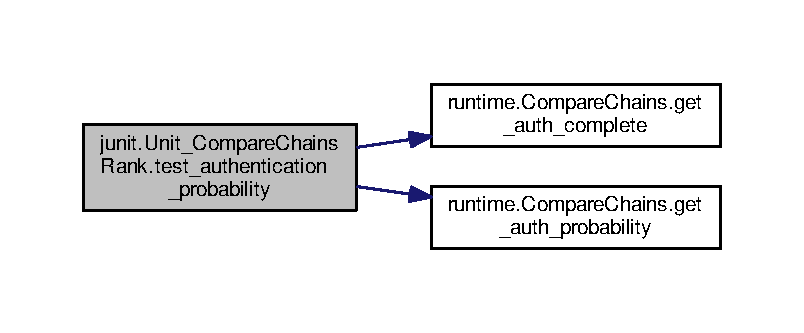
\includegraphics[width=350pt]{classjunit_1_1_unit___compare_chains_rank_adecfca92c2f0fb546dc44d77285d37d6_cgraph}
\end{center}
\end{figure}




The documentation for this class was generated from the following file\+:\begin{DoxyCompactItemize}
\item 
/home/element/\+P\+U\+F/\+Keyboard/java\+\_\+scripts/java\+\_\+marcov\+\_\+model/src/junit/\hyperlink{_unit___compare_chains_rank_8java}{Unit\+\_\+\+Compare\+Chains\+Rank.\+java}\end{DoxyCompactItemize}

\hypertarget{classjunit_1_1_unit___complete_probability}{}\section{junit.\+Unit\+\_\+\+Complete\+Probability Class Reference}
\label{classjunit_1_1_unit___complete_probability}\index{junit.\+Unit\+\_\+\+Complete\+Probability@{junit.\+Unit\+\_\+\+Complete\+Probability}}


unit test demonstrating how to compute probility  


\subsection*{Public Member Functions}
\begin{DoxyCompactItemize}
\item 
void \hyperlink{classjunit_1_1_unit___complete_probability_aefbaa874bac003953a07d88aed5cf3df}{init} ()
\item 
void \hyperlink{classjunit_1_1_unit___complete_probability_aebf3c4155ae93be00b46e5cff5f98715}{test\+\_\+replica\+\_\+distribution} ()
\begin{DoxyCompactList}\small\item\em test different properties of replica chain to see if this works as expected. \end{DoxyCompactList}\end{DoxyCompactItemize}


\subsection{Detailed Description}
unit test demonstrating how to compute probility 

\subsection{Member Function Documentation}
\index{junit\+::\+Unit\+\_\+\+Complete\+Probability@{junit\+::\+Unit\+\_\+\+Complete\+Probability}!init@{init}}
\index{init@{init}!junit\+::\+Unit\+\_\+\+Complete\+Probability@{junit\+::\+Unit\+\_\+\+Complete\+Probability}}
\subsubsection[{\texorpdfstring{init()}{init()}}]{\setlength{\rightskip}{0pt plus 5cm}void junit.\+Unit\+\_\+\+Complete\+Probability.\+init (
\begin{DoxyParamCaption}
{}
\end{DoxyParamCaption}
)}\hypertarget{classjunit_1_1_unit___complete_probability_aefbaa874bac003953a07d88aed5cf3df}{}\label{classjunit_1_1_unit___complete_probability_aefbaa874bac003953a07d88aed5cf3df}


Here is the call graph for this function\+:\nopagebreak
\begin{figure}[H]
\begin{center}
\leavevmode
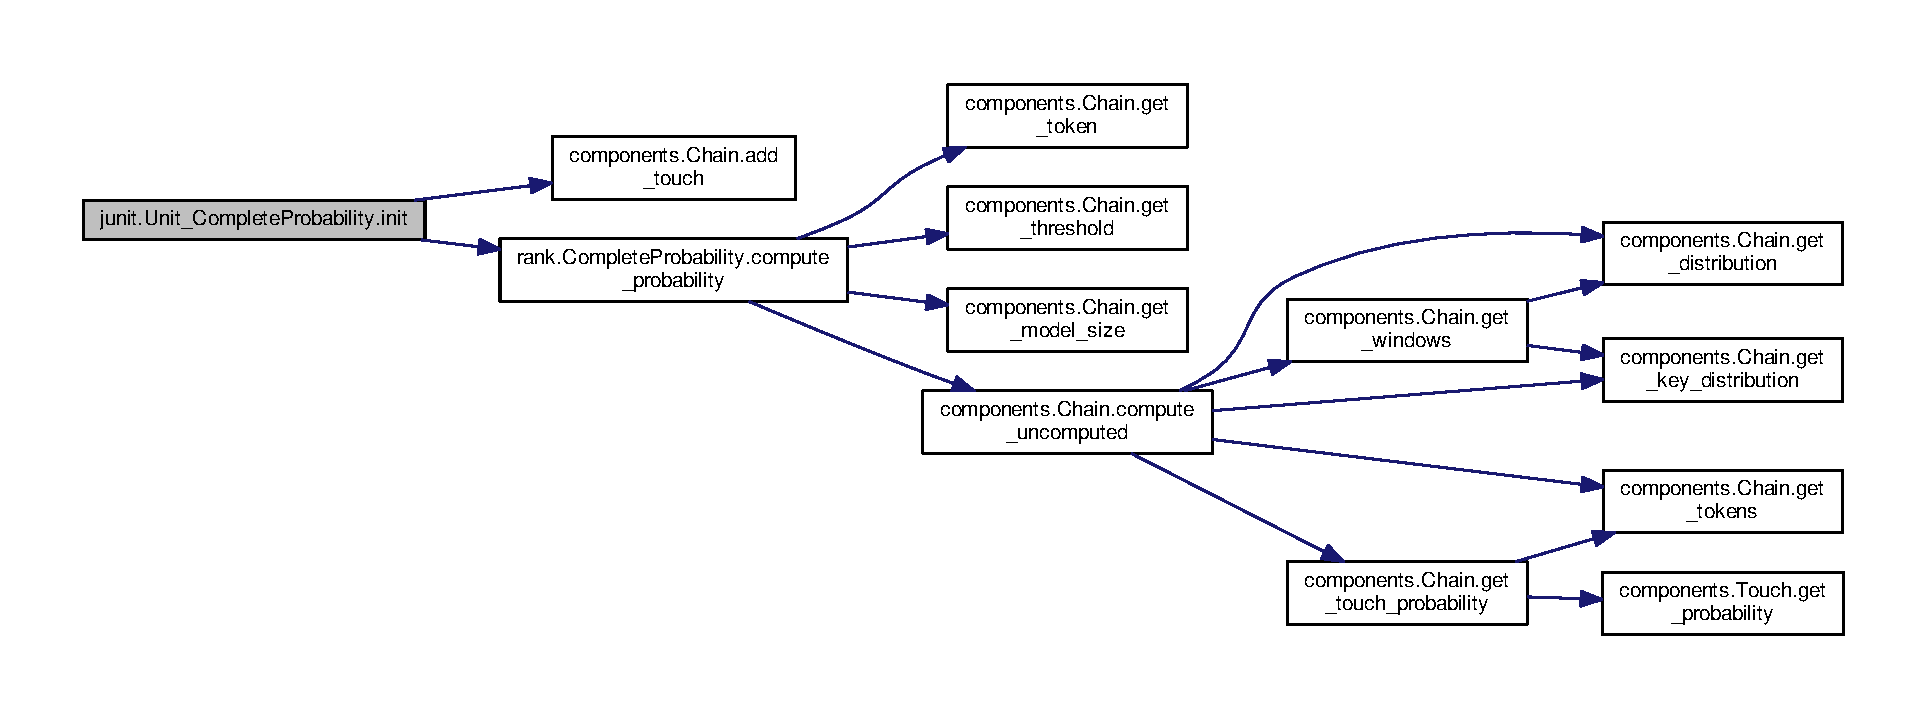
\includegraphics[width=350pt]{classjunit_1_1_unit___complete_probability_aefbaa874bac003953a07d88aed5cf3df_cgraph}
\end{center}
\end{figure}


\index{junit\+::\+Unit\+\_\+\+Complete\+Probability@{junit\+::\+Unit\+\_\+\+Complete\+Probability}!test\+\_\+replica\+\_\+distribution@{test\+\_\+replica\+\_\+distribution}}
\index{test\+\_\+replica\+\_\+distribution@{test\+\_\+replica\+\_\+distribution}!junit\+::\+Unit\+\_\+\+Complete\+Probability@{junit\+::\+Unit\+\_\+\+Complete\+Probability}}
\subsubsection[{\texorpdfstring{test\+\_\+replica\+\_\+distribution()}{test_replica_distribution()}}]{\setlength{\rightskip}{0pt plus 5cm}void junit.\+Unit\+\_\+\+Complete\+Probability.\+test\+\_\+replica\+\_\+distribution (
\begin{DoxyParamCaption}
{}
\end{DoxyParamCaption}
)}\hypertarget{classjunit_1_1_unit___complete_probability_aebf3c4155ae93be00b46e5cff5f98715}{}\label{classjunit_1_1_unit___complete_probability_aebf3c4155ae93be00b46e5cff5f98715}


test different properties of replica chain to see if this works as expected. 

Replica chain should contain the probabilities for when window is equal to 1. 

Here is the call graph for this function\+:\nopagebreak
\begin{figure}[H]
\begin{center}
\leavevmode
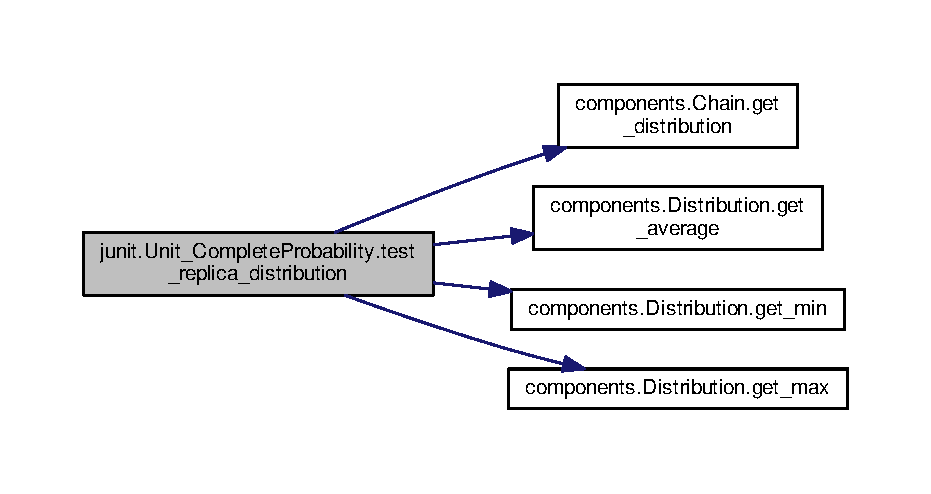
\includegraphics[width=350pt]{classjunit_1_1_unit___complete_probability_aebf3c4155ae93be00b46e5cff5f98715_cgraph}
\end{center}
\end{figure}




The documentation for this class was generated from the following file\+:\begin{DoxyCompactItemize}
\item 
/home/element/\+P\+U\+F/\+Keyboard/java\+\_\+scripts/java\+\_\+marcov\+\_\+model/src/junit/\hyperlink{_unit___complete_probability_8java}{Unit\+\_\+\+Complete\+Probability.\+java}\end{DoxyCompactItemize}

\hypertarget{classtest_1_1_unit_compare_chains_rank}{}\section{test.\+Unit\+Compare\+Chains\+Rank Class Reference}
\label{classtest_1_1_unit_compare_chains_rank}\index{test.\+Unit\+Compare\+Chains\+Rank@{test.\+Unit\+Compare\+Chains\+Rank}}


J\+Unit test for testing Page\+Rank version of compairason Not that the Page\+Rank implementation is not currently functional.  




Collaboration diagram for test.\+Unit\+Compare\+Chains\+Rank\+:\nopagebreak
\begin{figure}[H]
\begin{center}
\leavevmode
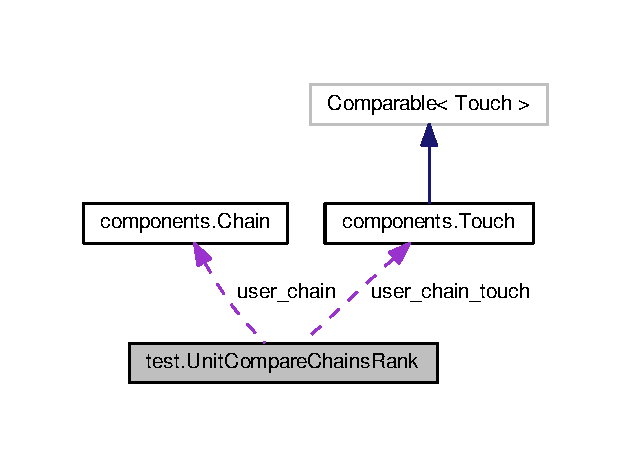
\includegraphics[width=303pt]{classtest_1_1_unit_compare_chains_rank__coll__graph}
\end{center}
\end{figure}
\subsection*{Public Member Functions}
\begin{DoxyCompactItemize}
\item 
void \hyperlink{classtest_1_1_unit_compare_chains_rank_ab7ae1a458472adfbab1bad8059935793}{init} ()
\item 
void \hyperlink{classtest_1_1_unit_compare_chains_rank_a8232052f40f79380b50564cdb2606421}{test\+\_\+chain\+\_\+to\+\_\+graph} ()
\begin{DoxyCompactList}\small\item\em tests chain\+\_\+to\+\_\+graph method to make sure the chain is converted to a State\+Graph correctly. \end{DoxyCompactList}\item 
void \hyperlink{classtest_1_1_unit_compare_chains_rank_a523ac7aa11a1b7632cd74ee00bea158b}{test\+\_\+touch\+\_\+index} ()
\begin{DoxyCompactList}\small\item\em make sure touch index returns the correct index in the list \end{DoxyCompactList}\item 
void \hyperlink{classtest_1_1_unit_compare_chains_rank_afe149cf20ab27d623f421175b92c3d88}{test\+\_\+touch\+\_\+window} ()
\begin{DoxyCompactList}\small\item\em make sure the touch\+\_\+window() returns the correct window in chain. \end{DoxyCompactList}\item 
void \hyperlink{classtest_1_1_unit_compare_chains_rank_a5a67766addc36792cf35a251dd0b6aee}{test} ()
\begin{DoxyCompactList}\small\item\em example test \end{DoxyCompactList}\end{DoxyCompactItemize}


\subsection{Detailed Description}
J\+Unit test for testing Page\+Rank version of compairason Not that the Page\+Rank implementation is not currently functional. 

\subsection{Member Function Documentation}
\index{test\+::\+Unit\+Compare\+Chains\+Rank@{test\+::\+Unit\+Compare\+Chains\+Rank}!init@{init}}
\index{init@{init}!test\+::\+Unit\+Compare\+Chains\+Rank@{test\+::\+Unit\+Compare\+Chains\+Rank}}
\subsubsection[{\texorpdfstring{init()}{init()}}]{\setlength{\rightskip}{0pt plus 5cm}void test.\+Unit\+Compare\+Chains\+Rank.\+init (
\begin{DoxyParamCaption}
{}
\end{DoxyParamCaption}
)}\hypertarget{classtest_1_1_unit_compare_chains_rank_ab7ae1a458472adfbab1bad8059935793}{}\label{classtest_1_1_unit_compare_chains_rank_ab7ae1a458472adfbab1bad8059935793}


Here is the call graph for this function\+:\nopagebreak
\begin{figure}[H]
\begin{center}
\leavevmode
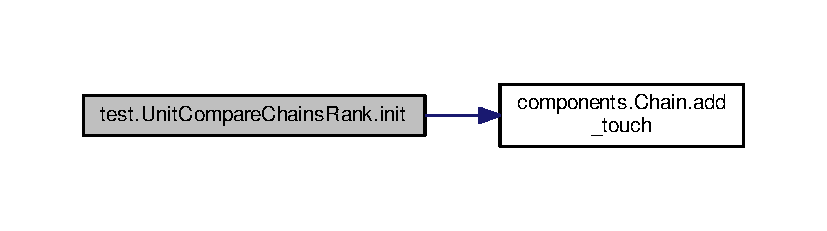
\includegraphics[width=350pt]{classtest_1_1_unit_compare_chains_rank_ab7ae1a458472adfbab1bad8059935793_cgraph}
\end{center}
\end{figure}


\index{test\+::\+Unit\+Compare\+Chains\+Rank@{test\+::\+Unit\+Compare\+Chains\+Rank}!test@{test}}
\index{test@{test}!test\+::\+Unit\+Compare\+Chains\+Rank@{test\+::\+Unit\+Compare\+Chains\+Rank}}
\subsubsection[{\texorpdfstring{test()}{test()}}]{\setlength{\rightskip}{0pt plus 5cm}void test.\+Unit\+Compare\+Chains\+Rank.\+test (
\begin{DoxyParamCaption}
{}
\end{DoxyParamCaption}
)}\hypertarget{classtest_1_1_unit_compare_chains_rank_a5a67766addc36792cf35a251dd0b6aee}{}\label{classtest_1_1_unit_compare_chains_rank_a5a67766addc36792cf35a251dd0b6aee}


example test 

\index{test\+::\+Unit\+Compare\+Chains\+Rank@{test\+::\+Unit\+Compare\+Chains\+Rank}!test\+\_\+chain\+\_\+to\+\_\+graph@{test\+\_\+chain\+\_\+to\+\_\+graph}}
\index{test\+\_\+chain\+\_\+to\+\_\+graph@{test\+\_\+chain\+\_\+to\+\_\+graph}!test\+::\+Unit\+Compare\+Chains\+Rank@{test\+::\+Unit\+Compare\+Chains\+Rank}}
\subsubsection[{\texorpdfstring{test\+\_\+chain\+\_\+to\+\_\+graph()}{test_chain_to_graph()}}]{\setlength{\rightskip}{0pt plus 5cm}void test.\+Unit\+Compare\+Chains\+Rank.\+test\+\_\+chain\+\_\+to\+\_\+graph (
\begin{DoxyParamCaption}
{}
\end{DoxyParamCaption}
)}\hypertarget{classtest_1_1_unit_compare_chains_rank_a8232052f40f79380b50564cdb2606421}{}\label{classtest_1_1_unit_compare_chains_rank_a8232052f40f79380b50564cdb2606421}


tests chain\+\_\+to\+\_\+graph method to make sure the chain is converted to a State\+Graph correctly. 

\index{test\+::\+Unit\+Compare\+Chains\+Rank@{test\+::\+Unit\+Compare\+Chains\+Rank}!test\+\_\+touch\+\_\+index@{test\+\_\+touch\+\_\+index}}
\index{test\+\_\+touch\+\_\+index@{test\+\_\+touch\+\_\+index}!test\+::\+Unit\+Compare\+Chains\+Rank@{test\+::\+Unit\+Compare\+Chains\+Rank}}
\subsubsection[{\texorpdfstring{test\+\_\+touch\+\_\+index()}{test_touch_index()}}]{\setlength{\rightskip}{0pt plus 5cm}void test.\+Unit\+Compare\+Chains\+Rank.\+test\+\_\+touch\+\_\+index (
\begin{DoxyParamCaption}
{}
\end{DoxyParamCaption}
)}\hypertarget{classtest_1_1_unit_compare_chains_rank_a523ac7aa11a1b7632cd74ee00bea158b}{}\label{classtest_1_1_unit_compare_chains_rank_a523ac7aa11a1b7632cd74ee00bea158b}


make sure touch index returns the correct index in the list 

\index{test\+::\+Unit\+Compare\+Chains\+Rank@{test\+::\+Unit\+Compare\+Chains\+Rank}!test\+\_\+touch\+\_\+window@{test\+\_\+touch\+\_\+window}}
\index{test\+\_\+touch\+\_\+window@{test\+\_\+touch\+\_\+window}!test\+::\+Unit\+Compare\+Chains\+Rank@{test\+::\+Unit\+Compare\+Chains\+Rank}}
\subsubsection[{\texorpdfstring{test\+\_\+touch\+\_\+window()}{test_touch_window()}}]{\setlength{\rightskip}{0pt plus 5cm}void test.\+Unit\+Compare\+Chains\+Rank.\+test\+\_\+touch\+\_\+window (
\begin{DoxyParamCaption}
{}
\end{DoxyParamCaption}
)}\hypertarget{classtest_1_1_unit_compare_chains_rank_afe149cf20ab27d623f421175b92c3d88}{}\label{classtest_1_1_unit_compare_chains_rank_afe149cf20ab27d623f421175b92c3d88}


make sure the touch\+\_\+window() returns the correct window in chain. 



The documentation for this class was generated from the following file\+:\begin{DoxyCompactItemize}
\item 
/home/element/\+P\+U\+F/\+Keyboard/java\+\_\+scripts/java\+\_\+marcov\+\_\+model/src/test/\hyperlink{_unit_compare_chains_rank_8java}{Unit\+Compare\+Chains\+Rank.\+java}\end{DoxyCompactItemize}

\hypertarget{classtest_1_1_unit_rank_compare}{}\section{test.\+Unit\+Rank\+Compare Class Reference}
\label{classtest_1_1_unit_rank_compare}\index{test.\+Unit\+Rank\+Compare@{test.\+Unit\+Rank\+Compare}}
\subsection*{Public Member Functions}
\begin{DoxyCompactItemize}
\item 
void \hyperlink{classtest_1_1_unit_rank_compare_ae0b3fb1356fcac8e9cf4d9bf7f4f323a}{init} ()
\item 
void \hyperlink{classtest_1_1_unit_rank_compare_ac8fdeb295d6451a69577d1ebe8ce458c}{test\+\_\+compare\+\_\+correct} ()
\item 
void \hyperlink{classtest_1_1_unit_rank_compare_ae488cafc0902af68a01e2d670350ccee}{test\+\_\+auth\+\_\+probability} ()
\item 
void \hyperlink{classtest_1_1_unit_rank_compare_aa02abba5193ffdbbb3fa8ed9d0cbcfe6}{test} ()
\end{DoxyCompactItemize}


\subsection{Detailed Description}
Test the compairason with ranks

\begin{DoxyAuthor}{Author}
element 
\end{DoxyAuthor}


\subsection{Member Function Documentation}
\index{test\+::\+Unit\+Rank\+Compare@{test\+::\+Unit\+Rank\+Compare}!init@{init}}
\index{init@{init}!test\+::\+Unit\+Rank\+Compare@{test\+::\+Unit\+Rank\+Compare}}
\subsubsection[{\texorpdfstring{init()}{init()}}]{\setlength{\rightskip}{0pt plus 5cm}void test.\+Unit\+Rank\+Compare.\+init (
\begin{DoxyParamCaption}
{}
\end{DoxyParamCaption}
)}\hypertarget{classtest_1_1_unit_rank_compare_ae0b3fb1356fcac8e9cf4d9bf7f4f323a}{}\label{classtest_1_1_unit_rank_compare_ae0b3fb1356fcac8e9cf4d9bf7f4f323a}
\index{test\+::\+Unit\+Rank\+Compare@{test\+::\+Unit\+Rank\+Compare}!test@{test}}
\index{test@{test}!test\+::\+Unit\+Rank\+Compare@{test\+::\+Unit\+Rank\+Compare}}
\subsubsection[{\texorpdfstring{test()}{test()}}]{\setlength{\rightskip}{0pt plus 5cm}void test.\+Unit\+Rank\+Compare.\+test (
\begin{DoxyParamCaption}
{}
\end{DoxyParamCaption}
)}\hypertarget{classtest_1_1_unit_rank_compare_aa02abba5193ffdbbb3fa8ed9d0cbcfe6}{}\label{classtest_1_1_unit_rank_compare_aa02abba5193ffdbbb3fa8ed9d0cbcfe6}
example test \index{test\+::\+Unit\+Rank\+Compare@{test\+::\+Unit\+Rank\+Compare}!test\+\_\+auth\+\_\+probability@{test\+\_\+auth\+\_\+probability}}
\index{test\+\_\+auth\+\_\+probability@{test\+\_\+auth\+\_\+probability}!test\+::\+Unit\+Rank\+Compare@{test\+::\+Unit\+Rank\+Compare}}
\subsubsection[{\texorpdfstring{test\+\_\+auth\+\_\+probability()}{test_auth_probability()}}]{\setlength{\rightskip}{0pt plus 5cm}void test.\+Unit\+Rank\+Compare.\+test\+\_\+auth\+\_\+probability (
\begin{DoxyParamCaption}
{}
\end{DoxyParamCaption}
)}\hypertarget{classtest_1_1_unit_rank_compare_ae488cafc0902af68a01e2d670350ccee}{}\label{classtest_1_1_unit_rank_compare_ae488cafc0902af68a01e2d670350ccee}
check the test that the compare vectors are correct \index{test\+::\+Unit\+Rank\+Compare@{test\+::\+Unit\+Rank\+Compare}!test\+\_\+compare\+\_\+correct@{test\+\_\+compare\+\_\+correct}}
\index{test\+\_\+compare\+\_\+correct@{test\+\_\+compare\+\_\+correct}!test\+::\+Unit\+Rank\+Compare@{test\+::\+Unit\+Rank\+Compare}}
\subsubsection[{\texorpdfstring{test\+\_\+compare\+\_\+correct()}{test_compare_correct()}}]{\setlength{\rightskip}{0pt plus 5cm}void test.\+Unit\+Rank\+Compare.\+test\+\_\+compare\+\_\+correct (
\begin{DoxyParamCaption}
{}
\end{DoxyParamCaption}
)}\hypertarget{classtest_1_1_unit_rank_compare_ac8fdeb295d6451a69577d1ebe8ce458c}{}\label{classtest_1_1_unit_rank_compare_ac8fdeb295d6451a69577d1ebe8ce458c}
checks that the probabilities are correct 

The documentation for this class was generated from the following file\+:\begin{DoxyCompactItemize}
\item 
/home/element/\+P\+U\+F/\+Keyboard/java\+\_\+scripts/java\+\_\+marcov\+\_\+model/src/test/\hyperlink{_unit_rank_compare_8java}{Unit\+Rank\+Compare.\+java}\end{DoxyCompactItemize}

\hypertarget{classcomponents_1_1_window}{}\section{components.\+Window Class Reference}
\label{classcomponents_1_1_window}\index{components.\+Window@{components.\+Window}}


This class will store and provide functions for a single window within the model.  


Inheritance diagram for components.\+Window\+:\begin{figure}[H]
\begin{center}
\leavevmode
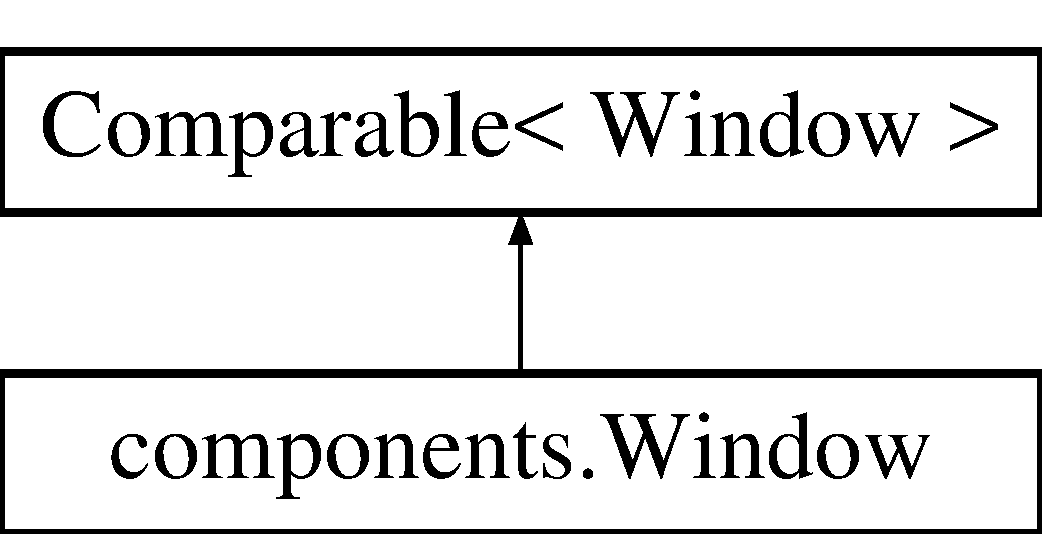
\includegraphics[height=2.000000cm]{classcomponents_1_1_window}
\end{center}
\end{figure}
\subsection*{Public Member Functions}
\begin{DoxyCompactItemize}
\item 
\hyperlink{classcomponents_1_1_window_a7ca5acd9fe649949cb0adccc837cf9d2}{Window} (List$<$ \hyperlink{classcomponents_1_1_touch}{Touch} $>$ touches)
\item 
\hyperlink{classcomponents_1_1_window_a5869fe4e3c5d711af934ff83114e55aa}{Window} (\hyperlink{classcomponents_1_1_window}{Window} w)
\begin{DoxyCompactList}\small\item\em copy constructor \end{DoxyCompactList}\item 
boolean \hyperlink{classcomponents_1_1_window_a3453a892128b5b4bded8bb7d18bbf35f}{compare\+\_\+with\+\_\+token} (List$<$ \hyperlink{classcomponents_1_1_token}{Token} $>$ tokens, \hyperlink{classcomponents_1_1_window}{Window} other\+\_\+window)
\item 
int \hyperlink{classcomponents_1_1_window_ab553fd43fb0240c0ef8a2218bdd5092c}{size} ()
\begin{DoxyCompactList}\small\item\em returns the number of touches in the window \end{DoxyCompactList}\item 
List$<$ \hyperlink{classcomponents_1_1_touch}{Touch} $>$ \hyperlink{classcomponents_1_1_window_abde5cba55b899aca32dd46750aeb4c32}{get\+\_\+touch\+\_\+list} ()
\begin{DoxyCompactList}\small\item\em returns the window in the form of a touch list \end{DoxyCompactList}\item 
int \hyperlink{classcomponents_1_1_window_aa733aef8f3ca04b19cd9fac71096a6ff}{hash\+Code} ()
\begin{DoxyCompactList}\small\item\em implement a hash function which returns the hash of the current window \end{DoxyCompactList}\item 
int \hyperlink{classcomponents_1_1_window_acf98290f4314388936c14de8b259339a}{compare\+To} (\hyperlink{classcomponents_1_1_window}{Window} other\+\_\+window)
\begin{DoxyCompactList}\small\item\em compare this window to another window. Return negative if this window is less than the other window. Comparason is based on touches\textquotesingle{} pressure. Returns 0 if they are equal. \end{DoxyCompactList}\item 
String \hyperlink{classcomponents_1_1_window_ab46581a7a83d26f3f7cbb8ef16cc68fc}{to\+String} ()
\end{DoxyCompactItemize}


\subsection{Detailed Description}
This class will store and provide functions for a single window within the model. 

\subsection{Constructor \& Destructor Documentation}
\index{components\+::\+Window@{components\+::\+Window}!Window@{Window}}
\index{Window@{Window}!components\+::\+Window@{components\+::\+Window}}
\subsubsection[{\texorpdfstring{Window(\+List$<$ Touch $>$ touches)}{Window(List< Touch > touches)}}]{\setlength{\rightskip}{0pt plus 5cm}components.\+Window.\+Window (
\begin{DoxyParamCaption}
\item[{List$<$ {\bf Touch} $>$}]{touches}
\end{DoxyParamCaption}
)}\hypertarget{classcomponents_1_1_window_a7ca5acd9fe649949cb0adccc837cf9d2}{}\label{classcomponents_1_1_window_a7ca5acd9fe649949cb0adccc837cf9d2}
\index{components\+::\+Window@{components\+::\+Window}!Window@{Window}}
\index{Window@{Window}!components\+::\+Window@{components\+::\+Window}}
\subsubsection[{\texorpdfstring{Window(\+Window w)}{Window(Window w)}}]{\setlength{\rightskip}{0pt plus 5cm}components.\+Window.\+Window (
\begin{DoxyParamCaption}
\item[{{\bf Window}}]{w}
\end{DoxyParamCaption}
)}\hypertarget{classcomponents_1_1_window_a5869fe4e3c5d711af934ff83114e55aa}{}\label{classcomponents_1_1_window_a5869fe4e3c5d711af934ff83114e55aa}


copy constructor 



\subsection{Member Function Documentation}
\index{components\+::\+Window@{components\+::\+Window}!compare\+\_\+with\+\_\+token@{compare\+\_\+with\+\_\+token}}
\index{compare\+\_\+with\+\_\+token@{compare\+\_\+with\+\_\+token}!components\+::\+Window@{components\+::\+Window}}
\subsubsection[{\texorpdfstring{compare\+\_\+with\+\_\+token(\+List$<$ Token $>$ tokens, Window other\+\_\+window)}{compare_with_token(List< Token > tokens, Window other_window)}}]{\setlength{\rightskip}{0pt plus 5cm}boolean components.\+Window.\+compare\+\_\+with\+\_\+token (
\begin{DoxyParamCaption}
\item[{List$<$ {\bf Token} $>$}]{tokens, }
\item[{{\bf Window}}]{other\+\_\+window}
\end{DoxyParamCaption}
)}\hypertarget{classcomponents_1_1_window_a3453a892128b5b4bded8bb7d18bbf35f}{}\label{classcomponents_1_1_window_a3453a892128b5b4bded8bb7d18bbf35f}
used for compairason of windows with a given token set. return true if this window is equal to auth window. \index{components\+::\+Window@{components\+::\+Window}!compare\+To@{compare\+To}}
\index{compare\+To@{compare\+To}!components\+::\+Window@{components\+::\+Window}}
\subsubsection[{\texorpdfstring{compare\+To(\+Window other\+\_\+window)}{compareTo(Window other_window)}}]{\setlength{\rightskip}{0pt plus 5cm}int components.\+Window.\+compare\+To (
\begin{DoxyParamCaption}
\item[{{\bf Window}}]{other\+\_\+window}
\end{DoxyParamCaption}
)}\hypertarget{classcomponents_1_1_window_acf98290f4314388936c14de8b259339a}{}\label{classcomponents_1_1_window_acf98290f4314388936c14de8b259339a}


compare this window to another window. Return negative if this window is less than the other window. Comparason is based on touches\textquotesingle{} pressure. Returns 0 if they are equal. 

\index{components\+::\+Window@{components\+::\+Window}!get\+\_\+touch\+\_\+list@{get\+\_\+touch\+\_\+list}}
\index{get\+\_\+touch\+\_\+list@{get\+\_\+touch\+\_\+list}!components\+::\+Window@{components\+::\+Window}}
\subsubsection[{\texorpdfstring{get\+\_\+touch\+\_\+list()}{get_touch_list()}}]{\setlength{\rightskip}{0pt plus 5cm}List$<${\bf Touch}$>$ components.\+Window.\+get\+\_\+touch\+\_\+list (
\begin{DoxyParamCaption}
{}
\end{DoxyParamCaption}
)}\hypertarget{classcomponents_1_1_window_abde5cba55b899aca32dd46750aeb4c32}{}\label{classcomponents_1_1_window_abde5cba55b899aca32dd46750aeb4c32}


returns the window in the form of a touch list 

\index{components\+::\+Window@{components\+::\+Window}!hash\+Code@{hash\+Code}}
\index{hash\+Code@{hash\+Code}!components\+::\+Window@{components\+::\+Window}}
\subsubsection[{\texorpdfstring{hash\+Code()}{hashCode()}}]{\setlength{\rightskip}{0pt plus 5cm}int components.\+Window.\+hash\+Code (
\begin{DoxyParamCaption}
{}
\end{DoxyParamCaption}
)}\hypertarget{classcomponents_1_1_window_aa733aef8f3ca04b19cd9fac71096a6ff}{}\label{classcomponents_1_1_window_aa733aef8f3ca04b19cd9fac71096a6ff}


implement a hash function which returns the hash of the current window 

\index{components\+::\+Window@{components\+::\+Window}!size@{size}}
\index{size@{size}!components\+::\+Window@{components\+::\+Window}}
\subsubsection[{\texorpdfstring{size()}{size()}}]{\setlength{\rightskip}{0pt plus 5cm}int components.\+Window.\+size (
\begin{DoxyParamCaption}
{}
\end{DoxyParamCaption}
)}\hypertarget{classcomponents_1_1_window_ab553fd43fb0240c0ef8a2218bdd5092c}{}\label{classcomponents_1_1_window_ab553fd43fb0240c0ef8a2218bdd5092c}


returns the number of touches in the window 

\index{components\+::\+Window@{components\+::\+Window}!to\+String@{to\+String}}
\index{to\+String@{to\+String}!components\+::\+Window@{components\+::\+Window}}
\subsubsection[{\texorpdfstring{to\+String()}{toString()}}]{\setlength{\rightskip}{0pt plus 5cm}String components.\+Window.\+to\+String (
\begin{DoxyParamCaption}
{}
\end{DoxyParamCaption}
)}\hypertarget{classcomponents_1_1_window_ab46581a7a83d26f3f7cbb8ef16cc68fc}{}\label{classcomponents_1_1_window_ab46581a7a83d26f3f7cbb8ef16cc68fc}


The documentation for this class was generated from the following file\+:\begin{DoxyCompactItemize}
\item 
/home/element/\+P\+U\+F/\+Keyboard/java\+\_\+scripts/java\+\_\+marcov\+\_\+model/src/components/\hyperlink{_window_8java}{Window.\+java}\end{DoxyCompactItemize}

\chapter{File Documentation}
\hypertarget{_chain_8java}{}\section{/home/element/\+P\+U\+F/\+Keyboard/java\+\_\+scripts/java\+\_\+marcov\+\_\+model/src/components/\+Chain.java File Reference}
\label{_chain_8java}\index{/home/element/\+P\+U\+F/\+Keyboard/java\+\_\+scripts/java\+\_\+marcov\+\_\+model/src/components/\+Chain.\+java@{/home/element/\+P\+U\+F/\+Keyboard/java\+\_\+scripts/java\+\_\+marcov\+\_\+model/src/components/\+Chain.\+java}}
\subsection*{Classes}
\begin{DoxyCompactItemize}
\item 
class \hyperlink{classcomponents_1_1_chain}{components.\+Chain}
\begin{DoxyCompactList}\small\item\em Markov \hyperlink{classcomponents_1_1_chain}{Chain} built using keyboard tokens. \end{DoxyCompactList}\end{DoxyCompactItemize}
\subsection*{Packages}
\begin{DoxyCompactItemize}
\item 
package \hyperlink{namespacecomponents}{components}
\end{DoxyCompactItemize}

\hypertarget{_distribution_8java}{}\section{/home/element/\+P\+U\+F/\+Keyboard/java\+\_\+scripts/java\+\_\+marcov\+\_\+model/src/components/\+Distribution.java File Reference}
\label{_distribution_8java}\index{/home/element/\+P\+U\+F/\+Keyboard/java\+\_\+scripts/java\+\_\+marcov\+\_\+model/src/components/\+Distribution.\+java@{/home/element/\+P\+U\+F/\+Keyboard/java\+\_\+scripts/java\+\_\+marcov\+\_\+model/src/components/\+Distribution.\+java}}
\subsection*{Classes}
\begin{DoxyCompactItemize}
\item 
class \hyperlink{classcomponents_1_1_distribution}{components.\+Distribution}
\begin{DoxyCompactList}\small\item\em Used to compute and store max, min, std\+\_\+deviation, and average for a list of \hyperlink{classcomponents_1_1_touch}{Touch}. \end{DoxyCompactList}\end{DoxyCompactItemize}
\subsection*{Packages}
\begin{DoxyCompactItemize}
\item 
package \hyperlink{namespacecomponents}{components}
\end{DoxyCompactItemize}

\hypertarget{_token_8java}{}\section{/home/element/\+P\+U\+F/\+Keyboard/java\+\_\+scripts/java\+\_\+marcov\+\_\+model/src/components/\+Token.java File Reference}
\label{_token_8java}\index{/home/element/\+P\+U\+F/\+Keyboard/java\+\_\+scripts/java\+\_\+marcov\+\_\+model/src/components/\+Token.\+java@{/home/element/\+P\+U\+F/\+Keyboard/java\+\_\+scripts/java\+\_\+marcov\+\_\+model/src/components/\+Token.\+java}}
\subsection*{Classes}
\begin{DoxyCompactItemize}
\item 
class \hyperlink{classcomponents_1_1_token}{components.\+Token}
\item 
enum \hyperlink{enumcomponents_1_1_token_1_1_type}{components.\+Token.\+Type}
\begin{DoxyCompactList}\small\item\em specify the type of token we want to build \end{DoxyCompactList}\end{DoxyCompactItemize}
\subsection*{Packages}
\begin{DoxyCompactItemize}
\item 
package \hyperlink{namespacecomponents}{components}
\end{DoxyCompactItemize}

\hypertarget{_touch_8java}{}\section{/home/element/\+P\+U\+F/\+Keyboard/java\+\_\+scripts/java\+\_\+marcov\+\_\+model/src/components/\+Touch.java File Reference}
\label{_touch_8java}\index{/home/element/\+P\+U\+F/\+Keyboard/java\+\_\+scripts/java\+\_\+marcov\+\_\+model/src/components/\+Touch.\+java@{/home/element/\+P\+U\+F/\+Keyboard/java\+\_\+scripts/java\+\_\+marcov\+\_\+model/src/components/\+Touch.\+java}}
\subsection*{Classes}
\begin{DoxyCompactItemize}
\item 
class \hyperlink{classcomponents_1_1_touch}{components.\+Touch}
\begin{DoxyCompactList}\small\item\em This class represents a touch event. \end{DoxyCompactList}\end{DoxyCompactItemize}
\subsection*{Packages}
\begin{DoxyCompactItemize}
\item 
package \hyperlink{namespacecomponents}{components}
\end{DoxyCompactItemize}

\hypertarget{_window_8java}{}\section{/home/element/\+P\+U\+F/\+Keyboard/java\+\_\+scripts/java\+\_\+marcov\+\_\+model/src/components/\+Window.java File Reference}
\label{_window_8java}\index{/home/element/\+P\+U\+F/\+Keyboard/java\+\_\+scripts/java\+\_\+marcov\+\_\+model/src/components/\+Window.\+java@{/home/element/\+P\+U\+F/\+Keyboard/java\+\_\+scripts/java\+\_\+marcov\+\_\+model/src/components/\+Window.\+java}}
\subsection*{Classes}
\begin{DoxyCompactItemize}
\item 
class \hyperlink{classcomponents_1_1_window}{components.\+Window}
\begin{DoxyCompactList}\small\item\em This class will store and provide functions for a single window within the model. \end{DoxyCompactList}\end{DoxyCompactItemize}
\subsection*{Packages}
\begin{DoxyCompactItemize}
\item 
package \hyperlink{namespacecomponents}{components}
\end{DoxyCompactItemize}

\hypertarget{_model__compare_8java}{}\section{/home/element/\+P\+U\+F/\+Keyboard/java\+\_\+scripts/java\+\_\+marcov\+\_\+model/src/data\+\_\+analysis/\+Model\+\_\+compare.java File Reference}
\label{_model__compare_8java}\index{/home/element/\+P\+U\+F/\+Keyboard/java\+\_\+scripts/java\+\_\+marcov\+\_\+model/src/data\+\_\+analysis/\+Model\+\_\+compare.\+java@{/home/element/\+P\+U\+F/\+Keyboard/java\+\_\+scripts/java\+\_\+marcov\+\_\+model/src/data\+\_\+analysis/\+Model\+\_\+compare.\+java}}
\subsection*{Classes}
\begin{DoxyCompactItemize}
\item 
class \hyperlink{classdata__analysis_1_1_model__compare}{data\+\_\+analysis.\+Model\+\_\+compare}
\begin{DoxyCompactList}\small\item\em Analysis class used to compare and analyze data gathered from users. \end{DoxyCompactList}\end{DoxyCompactItemize}
\subsection*{Packages}
\begin{DoxyCompactItemize}
\item 
package \hyperlink{namespacedata__analysis}{data\+\_\+analysis}
\end{DoxyCompactItemize}

\hypertarget{_model__compare__thread_8java}{}\section{/home/element/\+P\+U\+F/\+Keyboard/java\+\_\+scripts/java\+\_\+marcov\+\_\+model/src/data\+\_\+analysis/\+Model\+\_\+compare\+\_\+thread.java File Reference}
\label{_model__compare__thread_8java}\index{/home/element/\+P\+U\+F/\+Keyboard/java\+\_\+scripts/java\+\_\+marcov\+\_\+model/src/data\+\_\+analysis/\+Model\+\_\+compare\+\_\+thread.\+java@{/home/element/\+P\+U\+F/\+Keyboard/java\+\_\+scripts/java\+\_\+marcov\+\_\+model/src/data\+\_\+analysis/\+Model\+\_\+compare\+\_\+thread.\+java}}
\subsection*{Classes}
\begin{DoxyCompactItemize}
\item 
class \hyperlink{classdata__analysis_1_1_model__compare__thread}{data\+\_\+analysis.\+Model\+\_\+compare\+\_\+thread}
\end{DoxyCompactItemize}
\subsection*{Packages}
\begin{DoxyCompactItemize}
\item 
package \hyperlink{namespacedata__analysis}{data\+\_\+analysis}
\end{DoxyCompactItemize}

\hypertarget{_statistics_8java}{}\section{/home/element/\+P\+U\+F/\+Keyboard/java\+\_\+scripts/java\+\_\+marcov\+\_\+model/src/data\+\_\+analysis/\+Statistics.java File Reference}
\label{_statistics_8java}\index{/home/element/\+P\+U\+F/\+Keyboard/java\+\_\+scripts/java\+\_\+marcov\+\_\+model/src/data\+\_\+analysis/\+Statistics.\+java@{/home/element/\+P\+U\+F/\+Keyboard/java\+\_\+scripts/java\+\_\+marcov\+\_\+model/src/data\+\_\+analysis/\+Statistics.\+java}}
\subsection*{Classes}
\begin{DoxyCompactItemize}
\item 
class \hyperlink{classdata__analysis_1_1_statistics}{data\+\_\+analysis.\+Statistics}
\begin{DoxyCompactList}\small\item\em Generates statistics on results generated by model\+\_\+compare.\+java. \end{DoxyCompactList}\end{DoxyCompactItemize}
\subsection*{Packages}
\begin{DoxyCompactItemize}
\item 
package \hyperlink{namespacedata__analysis}{data\+\_\+analysis}
\end{DoxyCompactItemize}

\hypertarget{_marcov__console__panel_8java}{}\section{/home/element/\+P\+U\+F/\+Keyboard/java\+\_\+scripts/java\+\_\+marcov\+\_\+model/src/gui/\+Marcov\+\_\+console\+\_\+panel.java File Reference}
\label{_marcov__console__panel_8java}\index{/home/element/\+P\+U\+F/\+Keyboard/java\+\_\+scripts/java\+\_\+marcov\+\_\+model/src/gui/\+Marcov\+\_\+console\+\_\+panel.\+java@{/home/element/\+P\+U\+F/\+Keyboard/java\+\_\+scripts/java\+\_\+marcov\+\_\+model/src/gui/\+Marcov\+\_\+console\+\_\+panel.\+java}}
\subsection*{Classes}
\begin{DoxyCompactItemize}
\item 
class \hyperlink{classgui_1_1_marcov__console__panel}{gui.\+Marcov\+\_\+console\+\_\+panel}
\end{DoxyCompactItemize}
\subsection*{Packages}
\begin{DoxyCompactItemize}
\item 
package \hyperlink{namespacegui}{gui}
\end{DoxyCompactItemize}

\hypertarget{_marcov__file__display__panel_8java}{}\section{/home/element/\+P\+U\+F/\+Keyboard/java\+\_\+scripts/java\+\_\+marcov\+\_\+model/src/gui/\+Marcov\+\_\+file\+\_\+display\+\_\+panel.java File Reference}
\label{_marcov__file__display__panel_8java}\index{/home/element/\+P\+U\+F/\+Keyboard/java\+\_\+scripts/java\+\_\+marcov\+\_\+model/src/gui/\+Marcov\+\_\+file\+\_\+display\+\_\+panel.\+java@{/home/element/\+P\+U\+F/\+Keyboard/java\+\_\+scripts/java\+\_\+marcov\+\_\+model/src/gui/\+Marcov\+\_\+file\+\_\+display\+\_\+panel.\+java}}
\subsection*{Classes}
\begin{DoxyCompactItemize}
\item 
class \hyperlink{classgui_1_1_marcov__file__display__panel}{gui.\+Marcov\+\_\+file\+\_\+display\+\_\+panel}
\end{DoxyCompactItemize}
\subsection*{Packages}
\begin{DoxyCompactItemize}
\item 
package \hyperlink{namespacegui}{gui}
\end{DoxyCompactItemize}

\hypertarget{_marcov__frame_8java}{}\section{/home/element/\+P\+U\+F/\+Keyboard/java\+\_\+scripts/java\+\_\+marcov\+\_\+model/src/gui/\+Marcov\+\_\+frame.java File Reference}
\label{_marcov__frame_8java}\index{/home/element/\+P\+U\+F/\+Keyboard/java\+\_\+scripts/java\+\_\+marcov\+\_\+model/src/gui/\+Marcov\+\_\+frame.\+java@{/home/element/\+P\+U\+F/\+Keyboard/java\+\_\+scripts/java\+\_\+marcov\+\_\+model/src/gui/\+Marcov\+\_\+frame.\+java}}
\subsection*{Classes}
\begin{DoxyCompactItemize}
\item 
class \hyperlink{classgui_1_1_marcov__frame}{gui.\+Marcov\+\_\+frame}
\begin{DoxyCompactList}\small\item\em Display frame to contain buttons for running test code and panels to view results. \end{DoxyCompactList}\end{DoxyCompactItemize}
\subsection*{Packages}
\begin{DoxyCompactItemize}
\item 
package \hyperlink{namespacegui}{gui}
\end{DoxyCompactItemize}

\hypertarget{_marcov__options__panel_8java}{}\section{/home/element/\+P\+U\+F/\+Keyboard/java\+\_\+scripts/java\+\_\+marcov\+\_\+model/src/gui/\+Marcov\+\_\+options\+\_\+panel.java File Reference}
\label{_marcov__options__panel_8java}\index{/home/element/\+P\+U\+F/\+Keyboard/java\+\_\+scripts/java\+\_\+marcov\+\_\+model/src/gui/\+Marcov\+\_\+options\+\_\+panel.\+java@{/home/element/\+P\+U\+F/\+Keyboard/java\+\_\+scripts/java\+\_\+marcov\+\_\+model/src/gui/\+Marcov\+\_\+options\+\_\+panel.\+java}}
\subsection*{Classes}
\begin{DoxyCompactItemize}
\item 
class \hyperlink{classgui_1_1_marcov__options__panel}{gui.\+Marcov\+\_\+options\+\_\+panel}
\end{DoxyCompactItemize}
\subsection*{Packages}
\begin{DoxyCompactItemize}
\item 
package \hyperlink{namespacegui}{gui}
\end{DoxyCompactItemize}

\hypertarget{_start_g_u_i_8java}{}\section{/home/element/\+P\+U\+F/\+Keyboard/java\+\_\+scripts/java\+\_\+marcov\+\_\+model/src/gui/\+Start\+G\+UI.java File Reference}
\label{_start_g_u_i_8java}\index{/home/element/\+P\+U\+F/\+Keyboard/java\+\_\+scripts/java\+\_\+marcov\+\_\+model/src/gui/\+Start\+G\+U\+I.\+java@{/home/element/\+P\+U\+F/\+Keyboard/java\+\_\+scripts/java\+\_\+marcov\+\_\+model/src/gui/\+Start\+G\+U\+I.\+java}}
\subsection*{Classes}
\begin{DoxyCompactItemize}
\item 
class \hyperlink{classgui_1_1_start_g_u_i}{gui.\+Start\+G\+UI}
\begin{DoxyCompactList}\small\item\em G\+UI useful for testing. \end{DoxyCompactList}\end{DoxyCompactItemize}
\subsection*{Packages}
\begin{DoxyCompactItemize}
\item 
package \hyperlink{namespacegui}{gui}
\end{DoxyCompactItemize}

\hypertarget{_unit___compare_chains_rank_8java}{}\section{/home/element/\+P\+U\+F/\+Keyboard/java\+\_\+scripts/java\+\_\+marcov\+\_\+model/src/junit/\+Unit\+\_\+\+Compare\+Chains\+Rank.java File Reference}
\label{_unit___compare_chains_rank_8java}\index{/home/element/\+P\+U\+F/\+Keyboard/java\+\_\+scripts/java\+\_\+marcov\+\_\+model/src/junit/\+Unit\+\_\+\+Compare\+Chains\+Rank.\+java@{/home/element/\+P\+U\+F/\+Keyboard/java\+\_\+scripts/java\+\_\+marcov\+\_\+model/src/junit/\+Unit\+\_\+\+Compare\+Chains\+Rank.\+java}}
\subsection*{Classes}
\begin{DoxyCompactItemize}
\item 
class \hyperlink{classjunit_1_1_unit___compare_chains_rank}{junit.\+Unit\+\_\+\+Compare\+Chains\+Rank}
\begin{DoxyCompactList}\small\item\em goal is to test compare chains rank functionality \end{DoxyCompactList}\end{DoxyCompactItemize}
\subsection*{Packages}
\begin{DoxyCompactItemize}
\item 
package \hyperlink{namespacejunit}{junit}
\end{DoxyCompactItemize}

\hypertarget{_unit___complete_probability_8java}{}\section{/home/element/\+P\+U\+F/\+Keyboard/java\+\_\+scripts/java\+\_\+marcov\+\_\+model/src/junit/\+Unit\+\_\+\+Complete\+Probability.java File Reference}
\label{_unit___complete_probability_8java}\index{/home/element/\+P\+U\+F/\+Keyboard/java\+\_\+scripts/java\+\_\+marcov\+\_\+model/src/junit/\+Unit\+\_\+\+Complete\+Probability.\+java@{/home/element/\+P\+U\+F/\+Keyboard/java\+\_\+scripts/java\+\_\+marcov\+\_\+model/src/junit/\+Unit\+\_\+\+Complete\+Probability.\+java}}
\subsection*{Classes}
\begin{DoxyCompactItemize}
\item 
class \hyperlink{classjunit_1_1_unit___complete_probability}{junit.\+Unit\+\_\+\+Complete\+Probability}
\end{DoxyCompactItemize}
\subsection*{Packages}
\begin{DoxyCompactItemize}
\item 
package \hyperlink{namespacejunit}{junit}
\end{DoxyCompactItemize}

\hypertarget{_compare_chains_rank_8java}{}\section{/home/element/\+P\+U\+F/\+Keyboard/java\+\_\+scripts/java\+\_\+marcov\+\_\+model/src/rank/\+Compare\+Chains\+Rank.java File Reference}
\label{_compare_chains_rank_8java}\index{/home/element/\+P\+U\+F/\+Keyboard/java\+\_\+scripts/java\+\_\+marcov\+\_\+model/src/rank/\+Compare\+Chains\+Rank.\+java@{/home/element/\+P\+U\+F/\+Keyboard/java\+\_\+scripts/java\+\_\+marcov\+\_\+model/src/rank/\+Compare\+Chains\+Rank.\+java}}
\subsection*{Classes}
\begin{DoxyCompactItemize}
\item 
class \hyperlink{classrank_1_1_compare_chains_rank}{rank.\+Compare\+Chains\+Rank}
\end{DoxyCompactItemize}
\subsection*{Packages}
\begin{DoxyCompactItemize}
\item 
package \hyperlink{namespacerank}{rank}
\end{DoxyCompactItemize}

\hypertarget{_complete_probability_8java}{}\section{/home/element/\+P\+U\+F/\+Keyboard/java\+\_\+scripts/java\+\_\+marcov\+\_\+model/src/rank/\+Complete\+Probability.java File Reference}
\label{_complete_probability_8java}\index{/home/element/\+P\+U\+F/\+Keyboard/java\+\_\+scripts/java\+\_\+marcov\+\_\+model/src/rank/\+Complete\+Probability.\+java@{/home/element/\+P\+U\+F/\+Keyboard/java\+\_\+scripts/java\+\_\+marcov\+\_\+model/src/rank/\+Complete\+Probability.\+java}}
\subsection*{Classes}
\begin{DoxyCompactItemize}
\item 
class \hyperlink{classrank_1_1_complete_probability}{rank.\+Complete\+Probability}
\begin{DoxyCompactList}\small\item\em This class computes probability in a different way from what is contained in the Chain class. \end{DoxyCompactList}\end{DoxyCompactItemize}
\subsection*{Packages}
\begin{DoxyCompactItemize}
\item 
package \hyperlink{namespacerank}{rank}
\end{DoxyCompactItemize}

\hypertarget{_chain_builder_8java}{}\section{/home/element/\+P\+U\+F/\+Keyboard/java\+\_\+scripts/java\+\_\+marcov\+\_\+model/src/runtime/\+Chain\+Builder.java File Reference}
\label{_chain_builder_8java}\index{/home/element/\+P\+U\+F/\+Keyboard/java\+\_\+scripts/java\+\_\+marcov\+\_\+model/src/runtime/\+Chain\+Builder.\+java@{/home/element/\+P\+U\+F/\+Keyboard/java\+\_\+scripts/java\+\_\+marcov\+\_\+model/src/runtime/\+Chain\+Builder.\+java}}
\subsection*{Classes}
\begin{DoxyCompactItemize}
\item 
class \hyperlink{classruntime_1_1_chain_builder}{runtime.\+Chain\+Builder}
\begin{DoxyCompactList}\small\item\em Wrapper around Chain used to make using the model easier in a real application. \end{DoxyCompactList}\item 
enum \hyperlink{enumruntime_1_1_chain_builder_1_1_state}{runtime.\+Chain\+Builder.\+State}
\item 
enum \hyperlink{enumruntime_1_1_chain_builder_1_1_compare_method}{runtime.\+Chain\+Builder.\+Compare\+Method}
\end{DoxyCompactItemize}
\subsection*{Packages}
\begin{DoxyCompactItemize}
\item 
package \hyperlink{namespaceruntime}{runtime}
\end{DoxyCompactItemize}

\hypertarget{_compare_chains_8java}{}\section{/home/element/\+P\+U\+F/\+Keyboard/java\+\_\+scripts/java\+\_\+marcov\+\_\+model/src/runtime/\+Compare\+Chains.java File Reference}
\label{_compare_chains_8java}\index{/home/element/\+P\+U\+F/\+Keyboard/java\+\_\+scripts/java\+\_\+marcov\+\_\+model/src/runtime/\+Compare\+Chains.\+java@{/home/element/\+P\+U\+F/\+Keyboard/java\+\_\+scripts/java\+\_\+marcov\+\_\+model/src/runtime/\+Compare\+Chains.\+java}}
\subsection*{Classes}
\begin{DoxyCompactItemize}
\item 
class \hyperlink{classruntime_1_1_compare_chains}{runtime.\+Compare\+Chains}
\begin{DoxyCompactList}\small\item\em Use the compare method of the Chain class to determine an authetnication probability between 0 and 1. \end{DoxyCompactList}\end{DoxyCompactItemize}
\subsection*{Packages}
\begin{DoxyCompactItemize}
\item 
package \hyperlink{namespaceruntime}{runtime}
\end{DoxyCompactItemize}

\hypertarget{_operation__thread_8java}{}\section{/home/element/\+P\+U\+F/\+Keyboard/java\+\_\+scripts/java\+\_\+marcov\+\_\+model/src/runtime/\+Operation\+\_\+thread.java File Reference}
\label{_operation__thread_8java}\index{/home/element/\+P\+U\+F/\+Keyboard/java\+\_\+scripts/java\+\_\+marcov\+\_\+model/src/runtime/\+Operation\+\_\+thread.\+java@{/home/element/\+P\+U\+F/\+Keyboard/java\+\_\+scripts/java\+\_\+marcov\+\_\+model/src/runtime/\+Operation\+\_\+thread.\+java}}
\subsection*{Classes}
\begin{DoxyCompactItemize}
\item 
class \hyperlink{classruntime_1_1_operation__thread}{runtime.\+Operation\+\_\+thread}
\item 
enum \hyperlink{enumruntime_1_1_operation__thread_1_1_computation}{runtime.\+Operation\+\_\+thread.\+Computation}
\end{DoxyCompactItemize}
\subsection*{Packages}
\begin{DoxyCompactItemize}
\item 
package \hyperlink{namespaceruntime}{runtime}
\end{DoxyCompactItemize}

\hypertarget{_main_8java}{}\section{/home/element/\+P\+U\+F/\+Keyboard/java\+\_\+scripts/java\+\_\+marcov\+\_\+model/src/test/\+Main.java File Reference}
\label{_main_8java}\index{/home/element/\+P\+U\+F/\+Keyboard/java\+\_\+scripts/java\+\_\+marcov\+\_\+model/src/test/\+Main.\+java@{/home/element/\+P\+U\+F/\+Keyboard/java\+\_\+scripts/java\+\_\+marcov\+\_\+model/src/test/\+Main.\+java}}
\subsection*{Classes}
\begin{DoxyCompactItemize}
\item 
class \hyperlink{classtest_1_1_main}{test.\+Main}
\begin{DoxyCompactList}\small\item\em This class is used to test that the model is being built correctly. \end{DoxyCompactList}\item 
enum \hyperlink{enumtest_1_1_main_1_1_test_files_1_1_pressure_amount}{test.\+Main.\+Test\+Files.\+Pressure\+Amount}
\item 
enum \hyperlink{enumtest_1_1_main_1_1_test_files_1_1_distribution}{test.\+Main.\+Test\+Files.\+Distribution}
\item 
enum \hyperlink{enumtest_1_1_main_1_1_test_files_1_1_concentration}{test.\+Main.\+Test\+Files.\+Concentration}
\end{DoxyCompactItemize}
\subsection*{Packages}
\begin{DoxyCompactItemize}
\item 
package \hyperlink{namespacetest}{test}
\end{DoxyCompactItemize}

\hypertarget{_print__model_8java}{}\section{/home/element/\+P\+U\+F/\+Keyboard/java\+\_\+scripts/java\+\_\+marcov\+\_\+model/src/test/\+Print\+\_\+model.java File Reference}
\label{_print__model_8java}\index{/home/element/\+P\+U\+F/\+Keyboard/java\+\_\+scripts/java\+\_\+marcov\+\_\+model/src/test/\+Print\+\_\+model.\+java@{/home/element/\+P\+U\+F/\+Keyboard/java\+\_\+scripts/java\+\_\+marcov\+\_\+model/src/test/\+Print\+\_\+model.\+java}}
\subsection*{Classes}
\begin{DoxyCompactItemize}
\item 
class \hyperlink{classtest_1_1_print__model}{test.\+Print\+\_\+model}
\begin{DoxyCompactList}\small\item\em This class will print out the model constructed form the designated file. \end{DoxyCompactList}\end{DoxyCompactItemize}
\subsection*{Packages}
\begin{DoxyCompactItemize}
\item 
package \hyperlink{namespacetest}{test}
\end{DoxyCompactItemize}

\hypertarget{_unit_compare_chains_rank_8java}{}\section{/home/element/\+P\+U\+F/\+Keyboard/java\+\_\+scripts/java\+\_\+marcov\+\_\+model/src/test/\+Unit\+Compare\+Chains\+Rank.java File Reference}
\label{_unit_compare_chains_rank_8java}\index{/home/element/\+P\+U\+F/\+Keyboard/java\+\_\+scripts/java\+\_\+marcov\+\_\+model/src/test/\+Unit\+Compare\+Chains\+Rank.\+java@{/home/element/\+P\+U\+F/\+Keyboard/java\+\_\+scripts/java\+\_\+marcov\+\_\+model/src/test/\+Unit\+Compare\+Chains\+Rank.\+java}}
\subsection*{Classes}
\begin{DoxyCompactItemize}
\item 
class \hyperlink{classtest_1_1_unit_compare_chains_rank}{test.\+Unit\+Compare\+Chains\+Rank}
\begin{DoxyCompactList}\small\item\em J\+Unit test for testing Page\+Rank version of compairason Not that the Page\+Rank implementation is not currently functional. \end{DoxyCompactList}\end{DoxyCompactItemize}
\subsection*{Packages}
\begin{DoxyCompactItemize}
\item 
package \hyperlink{namespacetest}{test}
\end{DoxyCompactItemize}

\hypertarget{_unit_rank_compare_8java}{}\section{/home/element/\+P\+U\+F/\+Keyboard/java\+\_\+scripts/java\+\_\+marcov\+\_\+model/src/test/\+Unit\+Rank\+Compare.java File Reference}
\label{_unit_rank_compare_8java}\index{/home/element/\+P\+U\+F/\+Keyboard/java\+\_\+scripts/java\+\_\+marcov\+\_\+model/src/test/\+Unit\+Rank\+Compare.\+java@{/home/element/\+P\+U\+F/\+Keyboard/java\+\_\+scripts/java\+\_\+marcov\+\_\+model/src/test/\+Unit\+Rank\+Compare.\+java}}
\subsection*{Classes}
\begin{DoxyCompactItemize}
\item 
class \hyperlink{classtest_1_1_unit_rank_compare}{test.\+Unit\+Rank\+Compare}
\begin{DoxyCompactList}\small\item\em Test the compairason with ranks. \end{DoxyCompactList}\end{DoxyCompactItemize}
\subsection*{Packages}
\begin{DoxyCompactItemize}
\item 
package \hyperlink{namespacetest}{test}
\end{DoxyCompactItemize}

\hypertarget{_utilities_8java}{}\section{/home/element/\+P\+U\+F/\+Keyboard/java\+\_\+scripts/java\+\_\+marcov\+\_\+model/src/test/\+Utilities.java File Reference}
\label{_utilities_8java}\index{/home/element/\+P\+U\+F/\+Keyboard/java\+\_\+scripts/java\+\_\+marcov\+\_\+model/src/test/\+Utilities.\+java@{/home/element/\+P\+U\+F/\+Keyboard/java\+\_\+scripts/java\+\_\+marcov\+\_\+model/src/test/\+Utilities.\+java}}

\hypertarget{_trie_8java}{}\section{/home/element/\+P\+U\+F/\+Keyboard/java\+\_\+scripts/java\+\_\+marcov\+\_\+model/src/trie/\+Trie.java File Reference}
\label{_trie_8java}\index{/home/element/\+P\+U\+F/\+Keyboard/java\+\_\+scripts/java\+\_\+marcov\+\_\+model/src/trie/\+Trie.\+java@{/home/element/\+P\+U\+F/\+Keyboard/java\+\_\+scripts/java\+\_\+marcov\+\_\+model/src/trie/\+Trie.\+java}}
\subsection*{Classes}
\begin{DoxyCompactItemize}
\item 
class \hyperlink{classtrie_1_1_trie}{trie.\+Trie}
\begin{DoxyCompactList}\small\item\em Implementation of Prefix Tree. \end{DoxyCompactList}\item 
class {\bfseries trie.\+Trie.\+Trie\+Node}
\end{DoxyCompactItemize}
\subsection*{Packages}
\begin{DoxyCompactItemize}
\item 
package \hyperlink{namespacetrie}{trie}
\end{DoxyCompactItemize}

\hypertarget{_trie_list_8java}{}\section{/home/element/\+P\+U\+F/\+Keyboard/java\+\_\+scripts/java\+\_\+marcov\+\_\+model/src/trie/\+Trie\+List.java File Reference}
\label{_trie_list_8java}\index{/home/element/\+P\+U\+F/\+Keyboard/java\+\_\+scripts/java\+\_\+marcov\+\_\+model/src/trie/\+Trie\+List.\+java@{/home/element/\+P\+U\+F/\+Keyboard/java\+\_\+scripts/java\+\_\+marcov\+\_\+model/src/trie/\+Trie\+List.\+java}}
\subsection*{Classes}
\begin{DoxyCompactItemize}
\item 
class \hyperlink{classtrie_1_1_trie_list}{trie.\+Trie\+List}
\begin{DoxyCompactList}\small\item\em Wrapper around \hyperlink{classtrie_1_1_trie}{Trie} used to maintain an ordering among the stored elements. \end{DoxyCompactList}\end{DoxyCompactItemize}
\subsection*{Packages}
\begin{DoxyCompactItemize}
\item 
package \hyperlink{namespacetrie}{trie}
\end{DoxyCompactItemize}

%--- End generated contents ---

% Index
\backmatter
\newpage
\phantomsection
\clearemptydoublepage
\addcontentsline{toc}{chapter}{Index}
\printindex

\end{document}
